%%%%%%%%%%%%%%%%%%%%%%%%%%%%%%%%%%%%%%%%%%%%%%%%%%%%%%%%%%%%%%%%%%%%%%%%%%%%%%
% ASU Dissertation Template
%%%%%%%%%%%%%%%%%%%%%%%%%%%%%%%%%%%%%%%%%%%%%%%%%%%%%%%%%%%%%%%%%%%%%%%%%%%%%%
% Copyright 2015 Robert W. Kutter (robert@kutterconsulting.com)
%
%   See also: http://kutterconsulting.com
%
% For guidance on using this file, see the README.
%
%%%%%%%%%%%%%%%%%%%%%%%%%%%%%%%%%%%%%%%%%%%%%%%%%%%%%%%%%%%%%%%%%%%%%%%%%%%%%%
% Preamble
%%%%%%%%%%%%%%%%%%%%%%%%%%%%%%%%%%%%%%%%%%%%%%%%%%%%%%%%%%%%%%%%%%%%%%%%%%%%%%
\newcommand*{\pointsize}{12pt}          %<Set the font size; make sure the size is correct
                                        %   for the font you will use
\documentclass[letterpaper,             % Use US letter-size paper
               oneside,                 % No verso and recto differences
               \pointsize]              % Uses the font size defined above
               {memoir}
\renewcommand{\cleardoublepage}%        % \cleardoublepage will create entirely blank
  {\clearpage}%                         %   pages depending on settings (e.g., usually
                                        %   before start of \mainmatter); redefine it here
                                        %   so that no entirely blank pages are created
                                        %   automatically
%%%%%%%%%%%%%%%%%%%%%%%%%%%%%%%%%%%%%%%
% (Some) Packages
%%%%%%%%%%%%%%%%%%%%%%%%%%%%%%%%%%%%%%%
\usepackage{graphicx}                   % For importing image files
\usepackage{etoolbox}                   % For advanced commands throughout preamble
\usepackage{microtype}                  %~Improves kerning and protrusion (optional);
                                        %   See here for an introduction:
                                        %   http://www.khirevich.com/latex/microtype/

\providetoggle{usemicrotype}            % TRUE = microtype is being used
\makeatletter                           %   (Used to turn of microtype protrusion in the
\@ifpackageloaded{microtype}%           %   table of contents.)
  {\settoggle{usemicrotype}{true}}%
  {\settoggle{usemicrotype}{false}}
\makeatother
\usepackage{changepage}                 % For changing page layout (e.g., margins) in the
                                        %   middle of the document
\usepackage{calc}                       % Calculate text widths; used in page layout
                                        %   changes

%%%%%%%%%%%%%%%%%%%%%%%%%%%%%%%%%%%%%%%
% Title page, input
%%%%%%%%%%%%%%%%%%%%%%%%%%%%%%%%%%%%%%%
\listadd{\titlelines}%
  {Locating Arrays: Construction, Analysis, and Robustness} %<Enter the title of the dissertation
%\listadd{\titlelines}%
%  {Second Line of the Title}            % If you want to
                                        %   split the title across lines,
                                        %   use another \listadd command for the
                                        %   second line
\newcommand*\Author{Stephen Seidel} %<Enter your name; must match official transcript
\newcommand*{\documentname}%
  {Dissertation}                        %<Enter the type of document (capitalized)
\newcommand*{\degreename}
  {Master of Science}                   %<Enter the type of degree (capitalized)
\newcommand*\defdate{November 2018}        %<Give month (written out fully) and year of
                                        %   the oral defense
\listadd{\committeechair}{Violet R. Syrotiuk}   %<Enter committee chair name; use \listadd for
%\listadd{\committeechair}{Another name}%   for additional names
\newcommand*{\chairlabel}{Chair}        %<If you have co-chairs, replace this text with
                                        %   'Co-Chair'
\listadd{\committeemember}{Charles J. Colbourn} %<Enter committee member names; use \listadd for
\listadd{\committeemember}{Douglas C. Montgomery} %   additional names
\newcommand*{\gradmonth}{December}         %<Enter the graduation date; month can only be:
                                        %  May, August, or December
\newcommand*{\gradyear}{2018}           %<Enter the graduation year, e.g. 2014

\listadd{\keywords}{keyword 1}          %<Enter keywords; use \listadd for
\listadd{\keywords}{keyword 2}          %   additional names (up to 6)
\newcommand*{\graddate}{\gradmonth%     % Compose full graduation date
  \space\gradyear}

%%%%%%%%%%%%%%%%%%%%%%%%%%%%%%%%%%%%%%%
% Page layout
%%%%%%%%%%%%%%%%%%%%%%%%%%%%%%%%%%%%%%%
\settrimmedsize{\stockheight}%          % Specifies \paperheight and \paperwidth
  {\stockwidth}{*}
\settrims{0pt}{0pt}                     % Set location of page in relation to the stock.
                                        % Paper and stock size are equivalent,
                                        % so both \trimtop and \trimedge are set to 0pt
\newlength{\forfootskip}
\setlength{\forfootskip}%
  {3\baselineskip}
\newlength{\textblockheight}            % Calculate height of text block to leave room
\setlength{\textblockheight}{9.0in}     %   for footers, keeping page numbers outside
\addtolength{\textblockheight}%         %   the 1in vertical margins
  {-\forfootskip}
\settypeblocksize{\textblockheight}%    % Calculated by 1.0in vertical margins and
  {*}{*}                                %   letting margins set the width of the typeblock
\setulmargins{1.0in}{*}{*}              % Set upper margin (\uppermargin, not \topmargin);
                                        %   calculate the bottom margin
\setlrmarginsandblock{1.25in}{1.25in}{*}%~Set margins and calculate width of typeblock
\setheaderspaces{*}{0.5\baselineskip}{*}% Arguments: '\headdrop', '\headsep', and/or ratio
                                        %   Note: This is only used in the list of
                                        %   contents sections
\setheadfoot{\baselineskip}%            % Set '\headheight' and '\footskip'
  {\forfootskip}
\checkandfixthelayout                   % Required by memoir package after setting layout
\settypeoutlayoutunit{in}               % Write layout dimensions to log file in inches

%%%%%%%%%%%%%%%%%%%%%%%%%%%%%%%%%%%%%%%
% Fonts
%%%%%%%%%%%%%%%%%%%%%%%%%%%%%%%%%%%%%%%
\usepackage[T1]{fontenc}                % Standard option to handle, e.g., accented
                                        %   characters like 'ö' better
\usepackage{amssymb,mathtools}          % For AMS-LaTeX, see here for more:
                                        %     http://www.ams.org/publications/authors/tex/amslatex
                                        % ('mathtools' loads and extends 'amsmath')
\usepackage{ifxetex,ifluatex}           % Can check if XeTeX or LuaTeX was used to typeset
\usepackage{fixltx2e}                   % Provides \textsubscript
\IfFileExists{upquote.sty}%             % Use upquote if available, for
  {\usepackage{upquote}}{}              %   straight quotes in verbatim environments

% Load fonts depending on the
%   typesetting engine
\ifnum 0\ifxetex 1\fi\ifluatex 1\fi=0   % If pdftex
  \usepackage[utf8]{inputenc}           %   'utf8' should match the encoding of this file
                                        %
                                        %~Set up your font in pdftex here
                                        %
\else                                   % If xetex or luatex
  \ifxetex                              % If xetex
    \usepackage{mathspec}               % Matches non-math open-type font to math
                                        %   open-type font (use 'mathspec' if you want to
                                        %   write math in unicode)
    \usepackage{xunicode}               % Convert LaTeX character macros to unicode
  \else                                 % If luatex\usepackage{fontspec}
    \usepackage{fontspec}               % Use fontspec for (open type) font selection
  \fi
  \defaultfontfeatures{Mapping=tex-text,% Font spec setting
    Scale=MatchLowercase}
  \newcommand*{\euro}{€}
  \setmainfont{Garamond}                %<Set the main font; make sure the font is correct
                                        %   for the font size (See ASU Style Guide)
%  \setmathfont(Digits,Latin,Greek)%     %~Uncomment two lines to set a font for math%
%    {MATHFONT}
\fi

%%%%%%%%%%%%%%%%%%%%%%%%%%%%%%%%%%%%%%%
% Line spacing
%%%%%%%%%%%%%%%%%%%%%%%%%%%%%%%%%%%%%%%
\DoubleSpacing                         % True double spacing
\BeforeBeginEnvironment{quote}         % Memoir leaves most special material
  {\SingleSpacing}                     %   single spaced, but makes block quotes
\AfterEndEnvironment{quote}%           %   double-spaced; fix to follow ASU style guide
  {\vspace{-\baselineskip} %
  \DoubleSpacing}
\BeforeBeginEnvironment{quotation}%
  {\SingleSpacing}
\AfterEndEnvironment{quotation}%
  {\vspace{-\baselineskip} %
  \DoubleSpacing}

\setlength{\footnotesep}{\baselineskip}% Double space *between* footnotes
\renewcommand*{\footnoterule}{%        % Redefine footnoterule so that initial footnote
  \kern-3pt%                           %   still appears right under the rule (changing
  \hrule width 0.4\columnwidth         %   \footnotesep also changes the space between the
  \kern 2.6pt                          %   rule and the first footnote
  \vspace{-0.5\baselineskip}           % (Here is the vertical space adjustment)
  }

\usepackage{enumitem}                  % Control spacing in enumerate environment
\setlist{noitemsep}                    % Remove extra vertical spacing between items in lists
                                       % \setlist{nosep} to leave no space around whole list

%%%%%%%%%%%%%%%%%%%%%%%%%%%%%%%%%%%%%%%
% Page numbering
%%%%%%%%%%%%%%%%%%%%%%%%%%%%%%%%%%%%%%%
\makepagestyle{ASU}
  \makeevenfoot{ASU}{}{\thepage}{}
  \makeoddfoot{ASU}{}{\thepage}{}

%%%%%%%%%%%%%%%%%%%%%%%%%%%%%%%%%%%%%%%
% Title page, formatting
%%%%%%%%%%%%%%%%%%%%%%%%%%%%%%%%%%%%%%%
\newlength{\savedfootskip}
\setlength{\savedfootskip}{\footskip}
\newcommand{\titlepagesetup}{%          % Page layout for title page
  \changepage%                          % Adjustment to page dimensions:
    {\savedfootskip}%                   %   text height
    {}%                                 %   text width
    {}%                                 %   even-side margin
    {}%                                 %   odd-side margin
    {}%                                 %   column sep.
    {}%                                 %   topmargin
    {}%                                 %   headheight
    {}%                                 %   headsep
    {-\savedfootskip}%                  %   footskip
}

\newcommand{\closetitlepagesetup}{%     % Undo set up for title page
  \changepage{-\savedfootskip}{}{}{}{}%
    {}{}{}{\savedfootskip}%
}

\makeatletter                           % Do not modify this section; Enter info above
\newcommand*{\titlepageASU}{
  \titlepagesetup
  \clearpage
  \begin{center}
  \SingleSpacing
  \thispagestyle{empty}
    \renewcommand*{\do}[1]{##1 \\[\baselineskip]}
    \dolistloop{\titlelines}
    by \\[\baselineskip]
    \Author \\[4\baselineskip]
    A \documentname~Presented in Partial Fulfillment \\
    of the Requirements for the Degree \\
    \degreename \\
    \vfill                              % Vertically center the portion below
    Approved \defdate~by the \\
    Graduate Supervisory Committee: \\[\baselineskip]
    \renewcommand*{\do}[1]{##1, \chairlabel \\}
    \dolistloop{\committeechair}
    \renewcommand*{\do}[1]{##1 \\}
    \dolistloop{\committeemember}
    \vfill                              % Vertically center the portion above
    ARIZONA STATE UNIVERSITY \\[\baselineskip]
    \graddate
  \end{center}
  \clearpage
  \closetitlepagesetup
}
\makeatother

%%%%%%%%%%%%%%%%%%%%%%%%%%%%%%%%%%%%%%%
% Heading styles
%%%%%%%%%%%%%%%%%%%%%%%%%%%%%%%%%%%%%%%
% Note: memoir also has \book and \part commands; do not use these
\makechapterstyle{ASU}{%                % Define chapter heading style
  \renewcommand*{\chapterheadstart}{}   % Chapter title flush with top margin
  \renewcommand*{\chapnamefont}%        % Set font for 'Chapter' or 'Appendix'
    {\normalfont}
  \renewcommand*{\chapnumfont}%         % Set font for number in chapter headings
    {\normalfont}
  \renewcommand*{\afterchapternum}%     % Insert a double line break after
    {\\[\baselineskip]}                 %   chapter number
  \renewcommand*{\chaptitlefont}%       % Set font for chapter title name
    {\normalfont}
  \setlength{\afterchapskip}{0pt}       % Set vertical space between chapter title and
                                        %   first paragraph; equivalent to one line break
                                        %   (vertical space = \afterchapskip + \baselineskip)
                                        % Note: This \afterchapskip value is only used in
                                        %   front matter
  \renewcommand*{\printchapternum}{%    % Center justify chapter number
    \centering \chapnumfont %
    \thechapter}
  \renewcommand*{\printchaptertitle}[1]%% Center justify
    {\expandafter\centering %           %   \MakeUppercase has issues; see here for some
    \expandafter\chaptitlefont %        %   details: https://tex.stackexchange.com/questions/35680/uppercase-in-newcommand
    \expandafter\MakeUppercase %        %   Accented characters and some fonts may not
    \expandafter{##1}}                  %   uppercase correctly; if that happens, just
                                        %   type the chapter title in uppercase
}

\setsecnumdepth{all}                    %~Enter the levels that you want to have numbered
                                        %   (Default is to number all [5 levels deep].)

\newcommand{\divisionbeforeskip}%       % Create default formatting for headings
  {\baselineskip}
\newcommand{\divisionindent}%
  {0.5em}
\newcommand{\divisionfont}{\normalfont} % Font must be \normalfont
\newcommand{\divisionafterskip}%
  {\baselineskip}

\setbeforesecskip{\divisionbeforeskip}  % Apply default formatting to all heading levels
\setsecindent{\divisionindent}          % Note: If you change \setsecnumdepth above, you
\setsecheadstyle{\divisionfont}         %   will need to set the indent for all lower
\setaftersecskip{\divisionafterskip}    %   levels to '0pt'; otherwise, they will be
                                        %   preceded by unnecessary space
\setbeforesubsecskip{\divisionbeforeskip}
\setsubsecindent{\divisionindent}
\setsubsecheadstyle{\divisionfont}
\setaftersubsecskip{\divisionafterskip}

\setbeforesubsubsecskip{\divisionbeforeskip}
\setsubsubsecindent{\divisionindent}
\setsubsubsecheadstyle{\divisionfont}
\setaftersubsubsecskip{\divisionafterskip}

\setbeforeparaskip{\divisionbeforeskip}
\setparaindent{\divisionindent}
\setparaheadstyle{\divisionfont}
\setafterparaskip{\divisionafterskip}

\setbeforesubparaskip{\divisionbeforeskip}
\setsubparaindent{\divisionindent}
\setsubparaheadstyle{\divisionfont}
\setaftersubparaskip{\divisionafterskip}

%%%%%%%%%%%%%%%%%%%%%%%%%%%%%%%%%%%%%%%
% Paragraph formatting
%%%%%%%%%%%%%%%%%%%%%%%%%%%%%%%%%%%%%%%
%\sloppybottom                          % Reduce the chances of widows
\raggedbottom                           % Loosens vertical spacing requirements, so
                                        %   \sloppybottom doesn't make pages look bad;
                                        %   it also prevents large gaps in the middle of
                                        %   pages and pushes them to the bottom of pages
\indentafterchapter                     % Overrides the default which is not to indent
                                        %   the first paragraph in a chapter, but it
                                        %   looks odd in some places to not indent
                                        %   paragraphs

%%% List Titles %%%
\renewcommand{\contentsname}%           % Set heading for each list
  {Table of Contents}%                  %   Formatted as chapter headings by default, so
\renewcommand{\listtablename}%          %   no additional heading formatting is needed
  {List of Tables}
\renewcommand{\listfigurename}%
  {List of Figures}

%%% Depth %%%
\settocdepth{subparagraph}              % Include 5 levels deep (all levels) in TOC

%%% Fonts %%%
\makeatletter%
\patchcmd{\l@part}%                     % Patch the command that writes part-level entries
    {\cftpartfont {#1}}%                %   to the table of contents, so they are in
    {\normalfont \texorpdfstring{%      %   'normalfont' and uppercase
      \uppercase{#1}}{{#1}} }%
    {\typeout{Success: Patch %
      'l@part' to uppercase %
      part-level headings in the %
      table of contents.}}%
    {\typeout{Fail: Patch %
      'l@part' to uppercase %
      part-level headings in the %
      table of contents.}}%
\makeatother%

\makeatletter%
\patchcmd{\l@chapapp}%                  % Patch the command that writes chapter-level
    {\cftchapterfont {#1}}%             %   entries to the table of contents, so they are
    {\normalfont \texorpdfstring{%      %   in 'normalfont' and uppercase
      \uppercase{#1}}{{#1}} }%
    {\typeout{Success: Patch %
      'l@chapapp' to uppercase %
      part-level headings in the %
      table of contents.}}%
    {\typeout{Fail: Patch %
      'l@chapapp' to uppercase %
      part-level headings in the %
      table of contents.}}%
\makeatother%

% If not using 'hyperref', use the following commands to adjust 'part' and 'chapter'
%   level headings in the TOC
%\renewcommand*{\cftpartfont}%         % Uppercase 'part' and 'chapter' headings
%  {\normalfont\MakeTextUppercase}     % Note: Sending \MakeTextUppercase to the TOC
%\renewcommand*{\cftchapterfont}%      %   conflicts with hyperref and breaks it!
%  {\normalfont\MakeTextUppercase}%

\usepackage{titlecaps}                  % Set up headline style for captions in the
                                        %   lists of tables and figures
                                        % Note: ASU style guide does not provide
                                        %   comprehensive guidelines for headlines, so
                                        %   Chicago style for headline style is used
                                        % Note: Last word in title is not explicitly
                                        %   capitalized; in general, these settings are
                                        %   broadly correct, but captions should be
                                        %   reviewed to ensure they are being capitalized
                                        %   properly
\Resetlcwords
\Addlcwords{a an the}                   % Leave articles lowercase
\Addlcwords{and but for or nor}         % Leave conjunctions lowercase
\Addlcwords{aboard about above across % % Leave all prepositions lowercase
  after against along amid among anti % %   (This is a [non-exhaustive] list of common
  around as at before behind below %    %   one-word prepositions)
  beneath beside besides between %
  beyond but by concerning considering %
  despite down during except excepting %
  excluding following for from in %
  inside into like minus near of off %
  on onto opposite outside over past %
  per plus regarding round save since %
  than through to toward towards under %
  underneath unlike until up upon %
  versus vs via with within without}
\Addlcwords{ according\space{to} %      % Leave two-word conjunctions lowercase
  ahead\space{of} apart\space{from} %   %   (This is a [non-exhaustive] list of common
  as\space{for} as\space{of} %          %   two-word prepositions.)
  as\space{per} as\space{regards} %
  aside\space{from} astern\space{of} %
  back\space{to} because\space{of} %
  close\space{to} due\space{to} %
  except\space{for} far\space{from} %
  in\space{to} inside\space{of} %
  instead\space{of} left\space{of} %
  near\space{to} next\space{to} %
  on\space{to} opposite\space{of} %
  opposite\space{to} out\space{from} %
  out\space{of} outside\space{of} %
  owing\space{to} prior\space{to} %
  pursuant\space{to} rather\space{than} %
  regardless\space{of} right\space{of} %
  subsequent\space{to} such\space{as} %
  thanks\space{to} that\space{of} %
  up\space{to}}

\renewcommand{\cfttableaftersnumb}%     % Put table captions in List of Tables in title
  {\titlecap}%                          %   case
\renewcommand{\cftfigureaftersnumb}%    % Put table captions in List of Figures in title
  {\titlecap}%                          %   case

\newcommand{\macrocapwrap}[1]{%         % Use this macro to place other macros inside
  {\bgroup\bgroup{{#1}}\egroup\egroup}% %   captions, e.g., '\macrocapwrap{\ref{figure1}}'
}%                                      % Note: Necessary due to the 'titlecaps' package
                                        %   which modifies contents of captions

\renewcommand*{\cftpartpagefont}%       % Use normal font for all page numbers
  {\normalfont}
\renewcommand*{\cftchapterpagefont}%
  {\normalfont}
\renewcommand*{\cftsectionpagefont}%
  {\normalfont}
\renewcommand*{\cftsubsectionpagefont}%
  {\normalfont}
\renewcommand*{\cftsubsubsectionpagefont}%
  {\normalfont}
\renewcommand*{\cftsubsubsectionpagefont}%
  {\normalfont}
\renewcommand*{\cftparagraphpagefont}%
  {\normalfont}
\renewcommand*{\cftsubparagraphpagefont}%
  {\normalfont}
\renewcommand*{\cftfigurepagefont}%
  {\normalfont}
\renewcommand*{\cfttablepagefont}%
  {\normalfont}

\cftpagenumbersoff{part}                % Turn off page numbers for 'part's, which are
                                        %   actually serving as headings within the TOC

%%% Vertical Space %%%
\setlength{\cftbeforepartskip}{0pt}     % Remove all additional vertical spacing so TOC
\setlength{\cftbeforechapterskip}{0pt}  %   is double spaced uniformly
\setlength{\cftbeforesectionskip}{0pt}
\setlength{\cftbeforesubsectionskip}{0pt}
\setlength{\cftbeforesubsubsectionskip}{0pt}
\setlength{\cftbeforeparagraphskip}{0pt}
\setlength{\cftbeforesubparagraphskip}{0pt}
\setlength{\cftbeforefigureskip}{0pt}
\setlength{\cftbeforetableskip}{0pt}

\renewcommand{\insertchapterspace}{%    % By default, extra vertical space (10pt) is
  \addtocontents{lof}%                  %   inserted between tables and figures from
    {\protect\addvspace{0pt}}%          %   different chapters; remove this extra space.
  \addtocontents{lot}%
    {\protect\addvspace{0pt}}%
}

%%% Horizontal Space %%%
\newlength{\levelindentincrement}       % Set indent to increase by the same amount for
\setlength{\levelindentincrement}{2em}  %   each level in the TOC; don't adjust figure
\newlength{\levelindent}                %   or table indents
\setlength{\levelindent}%
  {\levelindentincrement}
\setlength{\cftchapterindent}%
  {\levelindent}
\addtolength{\levelindent}%
  {\levelindentincrement}
\setlength{\cftsectionindent}%
  {\levelindent}
\addtolength{\levelindent}%
  {\levelindentincrement}
\setlength{\cftsubsectionindent}%
  {\levelindent}
\addtolength{\levelindent}%
  {\levelindentincrement}
\setlength{\cftsubsubsectionindent}%
  {\levelindent}
\addtolength{\levelindent}%
  {\levelindentincrement}
\setlength{\cftparagraphindent}%
  {\levelindent}
\addtolength{\levelindent}%
  {\levelindentincrement}
\setlength{\cftsubparagraphindent}%
  {\levelindent}
\addtolength{\levelindent}%
  {\levelindentincrement}

\setlength{\cftchapternumwidth}%        % Decrease space between number and heading for
  {0.85\cftchapternumwidth}             %   all heading levels
\setlength{\cftsectionnumwidth}%
  {0.85\cftsectionnumwidth}
\setlength{\cftsubsectionnumwidth}%
  {0.85\cftsubsectionnumwidth}
\setlength{\cftsubsubsectionnumwidth}%
  {0.85\cftsubsubsectionnumwidth}
\setlength{\cftparagraphnumwidth}%
  {0.85\cftparagraphnumwidth}
\setlength{\cftsubparagraphnumwidth}%
  {0.85\cftsubparagraphnumwidth}
\setlength{\cftfigurenumwidth}%         % Figure has the same 'level' as 'chapter' in the
  {\cftchapternumwidth}                 %   figure list, so make the number spacing the
                                        %   same as for chapters
\setlength{\cfttablenumwidth}%          % Table has the same 'level' as 'chapter' in the
  {\cftchapternumwidth}                 %   table list, so make the number spacing the
                                        %   same as for chapters

%%% Leaders/dots %%%
\renewcommand*{\cftdotsep}{1.7}         % Set distance between dots for all heading levels
\renewcommand*{\cftchapterleader}%      % Turn on dots for 'chapter' level
  {\normalfont\cftdotfill{\cftdotsep}}
\makeatletter                           % Bring leader dots over to page number (no gap)
  \renewcommand{\@pnumwidth}{1.55em}    %~Manually adjust
  \renewcommand{\@tocrmarg}{2.55em}
\makeatother

\renewcommand{\cfttableaftersnum}{.}    % Period after number in LOT
\renewcommand{\cftfigureaftersnum}{.}   % Period after number in LOF

%%% Printing List Titles and Headers in Content Lists
% Table of Contents (TOC)
\copypagestyle{ASUtoc}{ASU}%            % Page style for regular page in TOC
  \makeevenhead{ASUtoc}%
    {\leftmark}{}{Page}
  \makeoddhead{ASUtoc}%
    {\leftmark}{}{Page}

\copypagestyle{ASUtocFirst}{ASU}%       % Custom page headers for first page of TOC
  \makeevenhead{ASUtocFirst}%           %    (print out the title)
    {}%
    {\printchaptertitle{\contentsname}}%
    {}
  \makeoddhead{ASUtocFirst}%
    {}%
    {\printchaptertitle{\contentsname}}%
    {}

\renewcommand{\tocheadstart}{}%         % Usually content list titles are printed like
                                        %   chapter headings; empty that formatting

\renewcommand{\printtoctitle}[1]{}%     % Don't print TOC title using default method;
                                        %   it will be output in the header

\renewcommand{\aftertoctitle}{%         % On the first page of the TOC, print out the
  \thispagestyle{ASUtocFirst}%          %   TOC title using a custom page style and print
  \hfill Page\par%                      %   the heading for the page below in the regular
  }%                                    %   textbox
                                        % Note: Need '\par' before lists; see here:
                                        % https://tex.stackexchange.com/questions/49882/yet-another-perhaps-a-missing-item-error

% List of Tables (LOT)
\copypagestyle{ASUlot}{ASU}%            % Page style for regular page in list of tables
  \makeevenhead{ASUlot}{Table}{}{Page}
  \makeoddhead{ASUlot}{Table}{}{Page}

\copypagestyle{ASUlotFirst}{ASU}%       % Custom page headers for first page of list of
  \makeevenhead{ASUlotFirst}%           %   tables (print out the title)
    {}%
    {\printchaptertitle{\listtablename}}%
    {}
  \makeoddhead{ASUlotFirst}%
    {}%
    {\printchaptertitle{\listtablename}}%
    {}

\renewcommand{\lotheadstart}{}%         % Usually content list titles are printed like
                                        %   chapter headings; empty that formatting;

\renewcommand{\printlottitle}[1]{}%     % Don't print LOT title using default method;
                                        %   it will be output in the header

\renewcommand{\afterlottitle}{%         % On the first page of the list of tables, print
  \thispagestyle{ASUlotFirst}%          %   out the title using a custom page style and
  Table\hfill Page\par}%                %   print heading below in regular textbox

% List of Figures (LOF)
\copypagestyle{ASUlof}{ASU}
  \makeevenhead{ASUlof}{Figure}{}{Page}
  \makeoddhead{ASUlof}{Figure}{}{Page}

\copypagestyle{ASUlofFirst}{ASU}%       % Custom page headers for first page of list of
  \makeevenhead{ASUlofFirst}%           %   figures (print out the title)
    {}%
    {\printchaptertitle{\listfigurename}}%
    {}
  \makeoddhead{ASUlofFirst}%
    {}%
    {\printchaptertitle{\listfigurename}}%
    {}

\renewcommand{\lofheadstart}{}%         % Usually content list titles are printed like
                                        %   chapter headings; empty that formatting

\renewcommand{\printloftitle}[1]{}%     % Don't print LOF title using default method;
                                        %   it will be output in the header

\renewcommand{\afterloftitle}{%         % On the first page of the list of figures, print
  \thispagestyle{ASUlofFirst}%          %   out the title using a custom page style and
  Figure\hfill Page\par}                %   print heading below in regular textbox

%%% Page layout (dimensions) for Contents Lists
\newlength{\verticalpush}               % Set up to change page dimensions for the table
                                        %   of contents
                                        % Push everything down so all the content is still
                                        %   1in from the top of the page, including the
                                        %   header, so the header is available for titles
                                        %   on the first page of contents lists and then
                                        %   the headings on subsequent pages
\setlength{\verticalpush}%              % Calculate difference between \headdrop and the
  {1.0in - \headdrop}                   %   total upper margin (1in), so you can push
                                        %   the top of the header down into the textbox

\newcommand{\contentslistsetup}{%       % Set up for contents lists
  \changepage%                          % Adjustment to page dimensions:
    {-\baselineskip}%                   %   text height
    {}%                                 %   text width
    {}%                                 %   even-side margin
    {}%                                 %   odd-side margin
    {}%                                 %   column sep.
    {\verticalpush}%                    %   topmargin
    {}%                                 %   headheight
    {}%                                 %   headsep
    {-\verticalpush+\baselineskip}%     %   footskip
}

\newcommand{\closecontentslistsetup}{%  % Undo set up for contents lists
  \changepage{\baselineskip}{}{}{}{}%
    {-\verticalpush}{}{}{\verticalpush-\baselineskip}%
}

% Content lists can also be output directly. If the following command were used, all the
%   headings would have to be output manually (i.e., can't rely on any memoir macros for
%   formatting or setting in contents lists headings and lists). It would be best to
%   create a custom macro, such as '\customtoc', to output headings and content lists
%   following the style guide.
%
% \makeatletter
%   \@starttoc{toc}
% \makeatother

% These pages partly explain why it's difficult to use 'afterpage' to change page layout
%   settings (essentially, it's because everything inside \afterpage has a local scope).
%   If it were possible to use 'afterpage' in that way, the content lists would  be
%   easier to format. A new page layout could be called after the first page of each
%   content  list. Instead, use page marks to get the layout required by the style guide.
% https://tex.stackexchange.com/questions/97126/attempts-to-manually-change-linewidth-ignored-by-latex
% https://tex.stackexchange.com/questions/85729/page-styles-only-work-for-thispagestyle-under-afterpage

%%%%%%%%%%%%%%%%%%%%%%%%%%%%%%%%%%%%%%%
% Footnotes and Endnotes
%%%%%%%%%%%%%%%%%%%%%%%%%%%%%%%%%%%%%%%
\usepackage{chngcntr}                   % Modify counters (e.g., for figures, footnotes)
\counterwithout*{footnote}{chapter}     % Make footnote numbering continuous throughout

\providetoggle{useendnotes}
\settoggle{useendnotes}{false}           %<Set to 'true' if you want to use endnotes
\iftoggle{useendnotes}{%                % Use the command \pagenote to create endnotes
                                        %   in the running text. They will be collected
                                        %   and printed in a 'Notes' section at the end
                                        %   of the document

  \makepagenote                         % Required in preamble if using endnotes
  \continuousnotenums                   % Numbering does *not* reset after each chapter
  \renewcommand*{\pagenotesubhead}[3]{} % No subheads inside note list (default is to
                                        %   divide them by chapter)
  \renewcommand*{\notenuminnotes}[1]%   % Remove extra space between note number and note
    {\normalfont #1.}                   %   text
  \renewcommand{\postnoteinnotes}%      % Double space *between* notes
    {\par\vspace{\baselineskip}}
}{}                                     % Do nothing here if not using endnotes

%%%%%%%%%%%%%%%%%%%%%%%%%%%%%%%%%%%%%%%
% Bibliography
%%%%%%%%%%%%%%%%%%%%%%%%%%%%%%%%%%%%%%%
\newcommand{\bibfilename}{library}      %<Enter the name of the *.bib file containing the
                                        %   reference information for sources cited in
                                        %   the text. God help you if you're doing
                                        %   citations manually.
\newcommand{\bibheading}{References}    %<Enter the heading for the references section:
                                        %   'References', 'Works Cited', or 'Bibliography'

\providetoggle{usebiblatex}             % True = a biblatex package is being used;
                                        %   False = 'natbib' is being used
\settoggle{usebiblatex}{true}           %~Set to 'false' to use 'natbib' intead of
                                        %   biblatex; I strongly recommend using biblatex
                                        %   because natbib is rather old and will break
                                        %   for innocuous things like underscores in URLs
\iftoggle{usebiblatex}{%                % Settings for citation package
%                                       % Settings for 'biblatex' or a version of
%                                       %   'biblatex'
  \usepackage[style=ieee]{biblatex}

  \bibliography{\bibfilename}
  \setlength{\bibitemsep}%              % Set vertical distance between
    {0.5\baselineskip}%                 %   bibliography entries
  \setcounter{biburlnumpenalty}{9000}   % Break URLs in bibliography across lines
  \setcounter{biburlucpenalty}{9000}
  \setcounter{biburllcpenalty}{9000}

  \usepackage[style=american,%          % Settings for quotation marks; load after
    english=american]{csquotes}%        %   'inputenc'; only use with biblatex; throws
  \MakeOuterQuote{"}%                   %   error when used with natbib
}{%                                     % Settings for 'natbib'
  \usepackage{natbib}%
  \newcommand{\natbibstyle}{asudis}%    %~Enter the name of the *.bst file to use to
                                        %   format citations with natbib. Default is
                                        %   'asudis'. I do not know where 'asudis' came
                                        %   from, but apparently it formats citations
                                        %   correctly because it was included with the
                                        %   previous LaTeX template.
}

%%%%%%%%%%%%%%%%%%%%%%%%%%%%%%%%%%%%%%%
% Tables and figures
%%%%%%%%%%%%%%%%%%%%%%%%%%%%%%%%%%%%%%%
\captiondelim{. }                       %~Use period (.) after caption number instead of
                                        %   colon (:). Change according to style guide.
\captionstyle[\raggedright]%            % Set justifcation for [one line captions]
  {\raggedright}                        %   and {multiple line captions}
\setlength{\belowcaptionskip}{0pt}      % Bring caption down closer to figure/table
\makeatletter                           % Consecutive numbering throughout
  \counterwithout{figure}{chapter}      %   (including back matter)
  \counterwithout{table}{chapter}
  \renewcommand\@memfront@floats{}
  \renewcommand\@memmain@floats{}
  \renewcommand\@memback@floats{}
\makeatletter

%%% Tables %%%
%
% Note: 'memoir' natively supports commands from the following table-related packages:
%   tabularx, ccaption, booktabs.
% Everyone has particular ideas about how tables should look, so you may need to
%   load additional packages and modify the code below to get tables (and figures) to
%   look the way you want them to.
\setfloatadjustment{table}{\raggedright}% Left justify material inside table floats
\usepackage{tabu}                       % 'tabu' is an excellent table package; it can
                                        %   automatically size column widths and has a
                                        %   lot of customizations that other packages do
                                        %   not. It also has a 'longtabu' environment that
                                        %   emulates 'longtable' with additional features
                                        %   from the 'tabu' package. If you don't want
                                        %   to use it, you can comment this line out.
\BeforeBeginEnvironment{table}%         % Single space inside table environment
  {\SingleSpacing}
\AfterEndEnvironment{table}
  {\DoubleSpacing}

%%% Figures %%%
\setfloatadjustment{figure}%            % Left justify material inside figure floats
  {\raggedright}
\BeforeBeginEnvironment{figure}%        % Single space inside figure environment
  {\SingleSpacing}
\AfterEndEnvironment{figure}
  {\DoubleSpacing}

\makeatletter                           % Define custom macro called '\maxwidth{}' that
  \def\maxwidth#1{%                     %   allows you to specify the maximum width of an
    \ifdim%                             %   imported image. See below for an example.
      \Gin@nat@width>#1 #1%             %
    \else%                              % Source: http://tex.stackexchange.com/questions/86350/includegraphics-maximum-width
      \Gin@nat@width%
    \fi}
\makeatother
%
% Example \maxwidth:
%
%   \includegraphics[width=\maxwidth]{\textwidth}]{image.pdf}
%
% Note: This will keep an image inside the horizontal margins assuming the image starts
%   on the right margin (i.e., no horizontal space before the image).

%%%%%%%%%%%%%%%%%%%%%%%%%%%%%%%%%%%%%%%
% Hyperref settings
%%%%%%%%%%%%%%%%%%%%%%%%%%%%%%%%%%%%%%%

%%% URL Settings %%%
\PassOptionsToPackage{hyphens}{url}
\usepackage[breaklinks=true]{hyperref}  % 'hyperref' should be loaded at the end of the
                                        %   preamble; Note: the uppercasing commands used
                                        %   throughout the preamble can conflict with it,
                                        %   especially when non-standard fonts or
                                        %   different file encodings are used
\urlstyle{same}                         % Set URLs in the same font as regular text

\tolerance 1414                         % Help URLs from entering margins
\hbadness 1414                          %   Source: https://tex.stackexchange.com/questions/3033/forcing-linebreaks-in-url
\emergencystretch 1.5em
\hfuzz 0.3pt
\widowpenalty=10000
\vfuzz \hfuzz

%%% Create metadata strings
\usepackage{hyperxmp}                   % For metadata
\renewcommand*{\do}[1]{#1\ }%           % Build title string to output to pdf document
\newcommand*{\onelinetitle}{%
  \dolistloop{\titlelines}%
}
\edef\theonelinetitle%
  {\onelinetitle}

\renewcommand*{\do}[1]{{#1}\ }%          % Build keyword string to output to pdf document
\newcommand*{\pdfkeywordsstring}{%
  \dolistloop{\keywords}%
}
\edef\thepdfkeywordsstring%
  {\pdfkeywordsstring}

\newcommand*{\pdfcopyrightstring}%      % Build copyright message string
  {Copyright \copyright\space\gradyear\ by \Author.%
  {\space}All rights reserved.}

\ifpdf                                  % Build pdf creator string (for pdfTeX)
  \makeatletter
  \def\extractpdftexversion#1-#2-#3 #4%
    \@nil{#3}
  \edef\pdfcreator{pdfTeX \expandafter%
    \extractpdftexversion\pdftexbanner\@nil}
  \makeatother
\fi
\ifxetex                                % Build pdf creator string (for XeTeX)
  \edef\pdfcreator{XeTeX %
    \the\XeTeXversion\XeTeXrevision}
\fi

\edef\pdfsummary{%                      % Build pdf summary
  A \documentname Presented in\space
  Partial Fulfillment of the\space
  Requirements for a \degreename\space
  from Arizona State University}

%%% Enter metadata and other settings
\hypersetup{                            % Set pdf metadata
  pdftitle={\theonelinetitle},          % Title
  pdfauthor={\Author},                  % Author
  pdfcreator={\pdfcreator},             % Enter the TeX writer for good documentation
 %pdfproducer={},                       % Let 'pdfproducer' be filled automatically
  pdfsubject={\pdfsummary},             % Subject of the document
  pdfkeywords=\thepdfkeywordsstring,    % List of keywords
  hidelinks={true},                     % Links look like regular text (no colors, boxes)
  breaklinks={true},                    % Allow links to break across lines
}
\ifxetex                                % If processing with XeTeX
  \hypersetup{unicode=true}             % Must use 'true' in XeTeX
\else
  \hypersetup{unicode=true}             % Default is to use 'true' otherwise, as well
\fi
\ifpdf                                  % Copyright message; probably only works in pdfTeX
  \hypersetup{
    pdfcopyright={\pdfcopyrightstring},
    pdfinfo={%
      Copyright=\pdfcopyrightstring%
    }%
  }
\fi

\usepackage%
  [numbered,%                           % Include numbers of sections in bookmarks
  open%                                 % Bookmark tree already expanded when PDF opened
  ]%
  {bookmark}
\bookmark[page=1,rellevel=0,%           % Create bookmark of title page at root level
  keeplevel=true]{Title Page}
\preto{\tableofcontents}{%              % Create bookmark for TOC
  \hypertarget{tocpage}{}%
  \bookmark[dest=tocpage,rellevel=0,%
    keeplevel=true]{\contentsname}%
}

%%%%%%%%%%%%%%%%%%%%%%%%%%%%%%%%%%%%%%%
% Copyright page
%%%%%%%%%%%%%%%%%%%%%%%%%%%%%%%%%%%%%%%
\newcommand{\copyrightpageASU}{%          % Create copyright page
  \thispagestyle{empty}
  \titlepagesetup
  ~\\ \vfill
    \begin{center}
      \copyright\gradyear\space%
      \Author\\%
      All Rights Reserved%
    \end{center}%
  \clearpage%
  \closetitlepagesetup
}

%%%%%%%%%%%%%%%%%%%%%%%%%%%%%%%%%%%%%%%
% Debugging Help
%%%%%%%%%%%%%%%%%%%%%%%%%%%%%%%%%%%%%%%
\usepackage{lipsum}                     % Outputs dummy text

%%%%%%%%%%%%%%%%%%%%%%%%%%%%%%%%%%%%%%%
% My packages and settings
%%%%%%%%%%%%%%%%%%%%%%%%%%%%%%%%%%%%%%%
\usepackage{longtable}
\usepackage{tabularx}
\newcolumntype{1}{>{\hsize=.1\hsize}X}
\newcolumntype{2}{>{\hsize=.2\hsize}X}
\newcolumntype{3}{>{\hsize=.3\hsize}X}
\newcolumntype{4}{>{\hsize=.4\hsize}X}
\newcolumntype{5}{>{\hsize=.5\hsize}X}
\newcolumntype{6}{>{\hsize=.6\hsize}X}
\newcolumntype{7}{>{\hsize=.7\hsize}X}
\newcolumntype{8}{>{\hsize=.8\hsize}X}
\newcolumntype{9}{>{\hsize=.9\hsize}X}

\usepackage{algorithm}
\usepackage{algorithmic}

\newcommand*\rot[1]{\rotatebox{90}{#1}}

%%%%%%%%%%%%%%%%%%%%%%%%%%%%%%%%%%%%%%%%%%%%%%%%%%%%%%%%%%%%%%%%%%%%%%%%%%%%%%%%
% END of my stuff
%%%%%%%%%%%%%%%%%%%%%%%%%%%%%%%%%%%%%%%%%%%%%%%%%%%%%%%%%%%%%%%%%%%%%%%%%%%%%%%%

%%%%%%%%%%%%%%%%%%%%%%%%%%%%%%%%%%%%%%%%%%%%%%%%%%%%%%%%%%%%%%%%%%%%%%%%%%%%%%
% Document
%%%%%%%%%%%%%%%%%%%%%%%%%%%%%%%%%%%%%%%%%%%%%%%%%%%%%%%%%%%%%%%%%%%%%%%%%%%%%%
\begin{document}

%%%%%%%%%%%%%%%%%%%%%%%%%%%%%%%%%%%%%%%
% Title page
%%%%%%%%%%%%%%%%%%%%%%%%%%%%%%%%%%%%%%%
\titlepageASU

%%%%%%%%%%%%%%%%%%%%%%%%%%%%%%%%%%%%%%%
% Copyright page
%%%%%%%%%%%%%%%%%%%%%%%%%%%%%%%%%%%%%%%
%\copyrightpageASU                       %~If you don't want to have a copyright page,
                                        %   comment out this line

%%%%%%%%%%%%%%%%%%%%%%%%%%%%%%%%%%%%%%%
% Front matter
%%%%%%%%%%%%%%%%%%%%%%%%%%%%%%%%%%%%%%%
\chapterstyle{ASU}
\pagestyle{ASU}
\frontmatter

\chapter*{Abstract}                     % Abstract is required
Modern computer systems are complex engineered systems involving a large collection of individual parts, each with many parameters, or factors, affecting system performance.
One way to understand these complex systems and their performance is through experimentation.
However, most modern computer systems involve such a large number of factors that thorough experimentation on all of them is impossible.
An initial screening step is thus necessary to determine which factors are relevant to the system's performance and which factors can be eliminated from experimentation.

Factors may impact system performance in different ways.
A factor at a specific level may significantly affect performance as a main effect, or in combination with other main effects as an interaction.
For screening, it is necessary both to identify the presence of these effects and to locate the factors responsible for them.
A locating array is a relatively new experimental design that causes every main effect and interaction to occur and distinguishes all sets of $d$ main effects and interactions from each other in the tests where they occur.
This design is therefore helpful in screening complex systems.

The process of screening using locating arrays involves multiple steps.
First, a locating array is constructed for all possibly significant factors.
Next, the system is executed for all tests indicated by the locating array and a response is observed.
Finally, the response is analyzed to identify the significant system factors for future experimentation.
However, simply constructing a reasonably sized locating array for a large system is no easy task and analyzing the response of the tests presents additional difficulties due to the large number of possible predictors and the inherent imbalance in the experimental design itself.
Further complications can arise from noise in the system or errors in testing.

This thesis has three contributions.
First, it provides an algorithm to construct locating arrays using the Lov{\'a}sz Local Lemma with Moser-Tardos resampling.
Second, it gives an algorithm to analyze the system response efficiently.
Finally, it studies the robustness of the analysis to the heavy-hitters assumption underlying the approach as well as to varying amounts of system noise.
                        %<Enter the name of the .tex file containing your
                                        %   your abstract or omit this line and type in
                                        %   your abstract here.

\chapter*{Dedication}                   %~Dedication is optional
%\clearpage                             %~If you don't wish to display the heading
                                        %   'Dedication', comment out the previous line
                                        %   and use this one instead.
\leavevmode\vfill
Here is a dummy dedication.
The dedication can be vertically centered like this text is.
See the \LaTeX\ code for this dedication to see how to vertically center the text of
your dedication.
\vfill
                      %<Enter the name of the .tex file containing your
                                        %   your dedication or omit this line and type in
                                        %   your dedication here.

\chapter*{Acknowledgments}              %~Acknowledgments are optional
Lorem ipsum dolor sit amet, consectetuer adipiscing elit. Ut purus elit, vestibulum ut,
placerat ac, adipiscing vitae, felis. Curabitur dictum gravida mauris. Nam arcu libero,
nonummy eget, consectetuer id, vulputate a, magna. Donec vehicula augue eu neque.
Pellentesque habitant morbi tristique senectus et netus et malesuada fames ac turpis
egestas. Mauris ut leo. Cras viverra metus rhoncus sem. Nulla et lectus vestibulum urna
fringilla ultrices. Phasellus eu tellus sit amet tortor gravida placerat. Integer sapien
est, iaculis in, pretium quis, viverra ac, nunc. Praesent eget sem vel leo ultrices
biben- dum. Aenean faucibus. Morbi dolor nulla, malesuada eu, pulvinar at, mollis ac,
nulla. Curabitur auctor semper nulla. Donec varius orci eget risus. Duis nibh mi,
congue eu, accumsan eleifend, sagittis quis, diam. Duis eget orci sit amet orci
dignissim rutrum.
                 %<Enter the name of the .tex file containing your
                                        %   acknowledgments or omit this line and type in
                                        %   your acknowledgments here.

\iftoggle{usemicrotype}                 % If 'microtype' is in use, turn off protrusion
  {\microtypesetup{protrusion=false}}%  %   for TOC
  {}
\clearpage                              % Output table of contents on a new page
\contentslistsetup                      % Change page layout for contents lists

\pagestyle{ASUtoc}
\tableofcontents*                       % Starred version leaves TOC heading out of TOC
\addtocontents{toc}%                    % List of ... needs to be on left margin, but
  {\setlength{\cftchapterindent}%       %   they inherit 'chapter' formatting, so override
    {0em}%
  }

\clearpage
\pagestyle{ASUlot}
\listoftables                           % List of Tables should appear in TOC, so use
                                        %   unstarred version of \listoftables
\clearpage
\pagestyle{ASUlof}
\listoffigures                          % List of Figures should appear in TOC, so use
                                        %   unstarred version of \listoffigures

\phantomsection                         % \phantomsection is needed before using
                                        %   \addtocontents when it contains certain macros
                                        %   when also using 'hyperref' package
\addtocontents{toc}%                    % Undo manual override above for chapter indent,
  {\setlength{\cftchapterindent}%       %   so actual chapters in the TOC are indented
    {\levelindentincrement}%            %   correctly
  }
\setlength{\afterchapskip}%             % Set vertical space between chapter title and
  {\baselineskip}                       %   first paragraph; equivalent to two line breaks

\phantomsection
\addcontentsline{toc}{part}{Chapter}    % Add "Chapter" to TOC here at 'part' level
\phantomsection
\addtocontents{toc}%                    % Add this 'mark' to TOC so subsequent pages use
  {\protect\markboth{CHAPTER}{Page}}    %   the "CHAPTER" heading

\iftoggle{usemicrotype}                 % If 'microtype' is in use, turn protrusion back
  {\microtypesetup{protrusion=true}}%   %   on
  {}

\clearpage                              % Note: All these changes have to be above a
                                        %   a '\clearpage' before '\mainmatter'

\pagestyle{ASU}                         % Switch back to regular page style for remainder
                                        %   of the document
\closecontentslistsetup                 % Undo page layout for contents lists

%\chapter{Definitions}                   %~OTHER LISTS (optional)
%\input{definitions}                     %<Enter the name of the .tex file or omit this
                                        %   line and type in here.

%\chapter{Preface}                       %~PREFACE (optional, less than 10 pages)
%\input{preface}                         %<Enter the name of the .tex file or omit this
                                        %   line and type in here.

%%%%%%%%%%%%%%%%%%%%%%%%%%%%%%%%%%%%%%%
% Body
%%%%%%%%%%%%%%%%%%%%%%%%%%%%%%%%%%%%%%%
\mainmatter
%\include{chapter1}                     %<Insert your chapters here; I recommend to use
%\include{chapter2}                     %   \include rather than \input for chapters
%\include{chapter3}% etc.
\chapter{Introduction} \label{chptr:introduction}

Large complex engineered systems involve many separate components interacting to ensure the proper functionality of the whole system.
Examples of these complex engineered systems are computer networks such as the internet.
Computer networks include separate components in many layers spanning from the physical to the application layer that all affect the proper functionality of the network.
There are parameters ({\em factors}) at every layer that can be adjusted to different values ({\em levels}) to affect the output ({\em response}) of the system.
Levels can therefore be assigned to the factors of the system, and a response can be observed.

Suppose we are interested in maximizing throughput for a particular network.
Many network factors at multiple layers can affect the response (the throughput of the network).
For example, the type of cable at the physical layer, the protocol at the transport layer, and the number of sockets at the application layer all might affect the network throughput.
The effects of these factors may be due to the assignment of a particular level to one factor ({\em main effect}), or it may be due to a combination of multiple assignments ({\em interaction}).
For example, the assignment of an optical fiber as the type of cable may significantly affect throughput as a main effect, while the combination of assigning TCP as the transport protocol and at the same time using a high number of sockets may significantly affect throughput as an interaction.
We refer to a factor or interaction as significant when its effects are noticeable over any noise in the system.

Experimentation is crucial to understanding the behavior of complex engineered systems, because analytical approaches are no longer feasible when the system is large.
But before experiments can be performed, we must determine the factors on which to perform the experimentation.
This initial step of choosing the significant factors to include in experimentation, and eliminating the insignificant factors, is known as {\em screening}.
In this work, we explore techniques for screening a large number of system factors, using initial experimentation with locating arrays, to determine the significant factors and interactions.
Once screening has been performed, further experimentation should be done on the significant factors to determine {\em how} they affect the system.
Our interest, however, is purely on the initial screening step that finds significant factors.

Similarly to \cite{CMjoco,seidelIWOCA}, we define $k$ system factors $F_1, F_2, \dots, F_k$.
Each factor $F_j$ has a set $L_j = \{v_{j1}, \dots, v_{j{\ell_j}}\}$ of $\ell_j$ possible levels (values).
A {\em test} is an assignment of a level from $L_j$ to $F_j$ for each factor.
For the purpose of conciseness, this work generally omits the factor index when referring to factor levels in assignments, i.e., we use $v_i$ instead of $v_{ji}$.
A {\em $t$-way interaction} in a test is any collection of $t$ assignments, and is said to have {\em strength} $t$.
An assignment of $v_{ji}$ to $F_j$ is written as $F_j = v_i$, and a $t$-way interaction is written as the $t$ assignments separated by $t - 1$ ampersands.
For example, $F_a = v_x$ \& $F_b = v_y$ is a 2-way interaction, and is said to have strength 2.
A main effect is a single assignment that is simply a 1-way interaction.
Each test therefore includes ({\em covers}) $k \choose t$ $t$-way interactions.
An {\em experimental design} of size $n$ is a collection of $n$ tests.
When running the system, a test results in one or more output response measurements.
An {\em experiment} consists of running the system for every test in the experimental design.
Usually, an experiment is represented as an $n \times k$ array, $A$, with tests corresponding to rows and factors corresponding to columns.
An element in the $i$-th row and $j$-th column contains a level from $L_j$ assigned to $F_j$ in the $i$-th test.
Following \cite{CMjoco}, for a $t$-way interaction $T$, denote the set of rows (tests) in $A$ where $T$ is covered as $\rho(A,T)$, and for a set $\mathcal{T}$ of interactions, define $\rho(A,\mathcal{T}) = \bigcup_{T \in {\mathcal{T}}} \rho(A,T)$.

Experimental designs used for screening fall into many different categories.
Full-factorial designs include all possible combinations of levels of each factor \cite{Montgomery-DOE-2017} and cover all $t$-way interactions where $1 \leq t \leq k$.
The size of a full-factorial design is exponential in the number of factors.
Fractional-factorial designs contain a fixed fraction of the tests in a full-factorial design and therefore also grow exponentially in the number of factors.
In general, complex engineered systems involve a large number of factors, making full-factorial and fractional-factorial experimental designs impractical for screening.

Saturated designs include a number of tests equal to one more than the number of factors \cite{Montgomery-DOE-2017}, i.e., $n = k + 1$.
Saturated designs are helpful when only a small fraction of the system factors are expected to contribute to the response.
Supersaturated designs employ even fewer tests than saturated designs \cite{Montgomery-DOE-2017}, i.e., $n < k + 1$.
While they are not widely used, supersaturated designs are potentially useful when very few factors are expected to contribute to the response \cite{Montgomery-DOE-2017}.
Both saturated and supersaturated designs conveniently involve running a small number of tests, but they only attempt to estimate main effects.
It may be impossible to estimate the effects of all interactions with these designs because a significant interaction may be missing completely from the design, or it may be indistinguishable from ({\em confounded} with) another interaction.
These designs often require advanced analysis techniques as well.

Covering arrays of strength $t$ are experimental designs that cover every $t$-way interaction in at least one test \cite{CMjoco}.
Covering arrays can reveal the presence of an interaction that has a significant impact on the system response, but they do not necessarily identify the specific significant interaction \cite{CMjoco}.
Suppose a system has $k = 3$ factors, $F_1, F_2, F_3$ and the number of levels are $\ell_1 = 2, \ell_2 = 3, \ell_3 = 3$.
Table \ref{tab:intro_ca} is a covering array $A$ of strength 2 for this system.
Define $T_1 = (F_3 = v_3$ \& $F_1 = v_2)$ and $T_2 = (F_3 = v_3$ \& $F_2 = v_2)$.
Then $\rho(A,T_1) = \{$4$\}$ and $\rho(A,T_2) = \{$4$\}$.
Suppose that $T_1$ is significant but $T_2$ is insignificant.
Thus test 4 produces a significantly different response (because of $T_1$) and the covering array reveals the {\em presence} of a significant interaction.
However, it is impossible to determine, from only the tests in Table \ref{tab:intro_ca}, whether $T_1$ or $T_2$ is significant (or if both are).
For the purpose of screening, we must determine the factors that are significant, and therefore must determine exactly which interaction is significant.

\begin{table}[htbp]
\caption{Covering Array - First Example}
\label{tab:intro_ca}
\begin{tabularx}{\textwidth}{|1|3|3|3|}
\hline
\multicolumn{4}{|c|}{Covering Array $A$} \\
\hline
Test & $F_1$ & $F_2$ & $F_3$ \\
\hline
 1 & $v_2$ & $v_3$ & $v_2$ \\
 2 & $v_2$ & $v_1$ & $v_1$ \\
 3 & $v_1$ & $v_1$ & $v_2$ \\
 4 & $v_2$ & $v_2$ & $v_3$ \\
 5 & $v_2$ & $v_3$ & $v_1$ \\
 6 & $v_1$ & $v_3$ & $v_3$ \\
 7 & $v_1$ & $v_2$ & $v_1$ \\
 8 & $v_2$ & $v_2$ & $v_2$ \\
 9 & $v_1$ & $v_1$ & $v_3$ \\
\hline
\end{tabularx}
\end{table}

This work focuses on using a new experimental design for screening - a {\em locating array} (LA) \cite{CMjoco}.
As discussed by Colbourn and McClary \cite{CMjoco}, an experimental design is $(d,t)$-{\em locating} if $\rho(A,\mathcal{T}_1) = \rho(A,\mathcal{T}_2) \Leftrightarrow \mathcal{T}_1 = \mathcal{T}_2$ whenever $\mathcal{T}_1, \mathcal{T}_2$ are any sets of $t$-way interactions where  $|\mathcal{T}_1| = d$, and $|\mathcal{T}_2| = d$.
When $|\mathcal{T}_1| \leq d$ and $|\mathcal{T}_2| \leq d$ and $\mathcal{T}_1, \mathcal{T}_2$ are any sets of interactions with strength at most $t$, the array is $(\overline{d},\overline{t})$-{\em locating}.
Thus while the covering array in Table \ref{tab:intro_ca} is unable to distinguish between $T_1$ and $T_2$ because $\rho(A,T_1)$ and $\rho(A,T_2)$ are equal, both a $(d,t)$ and $(\overline{d},\overline{t})$-locating array guarantee that $\rho(A,\mathcal{T}_1)$ and $\rho(A,\mathcal{T}_2)$ must be different when $\mathcal{T}_1$ and $\mathcal{T}_2$ are different sets.
For the purpose of screening, a locating array provides a set of tests to locate any set $\mathcal{T}$ of interactions that significantly affect the response.
Locating arrays are covering arrays with additional desirable properties, and are especially useful because they grow logarithmically in the number of factors when the number of levels is fixed for all factors \cite{CSmics}.

In this work, we focus on locating arrays where $d = 1$ because we make the assumption that the most significant interaction stands out in the response (more significant than all other significant interactions) and it is not necessary to locate more than one interaction at the same time.
We also assume that after the most significant interaction is located and its effect is removed from the response, then the second most significant interaction again stands out.
This assumption of a "heavy-hitters" pattern in the significant interactions has been used with locating arrays \cite{AldacoCS15,Compton-et-al-LA}, and is discussed in more detail in Chapter \ref{chptr:analysis} and tested in Chapter \ref{chptr:robustness}.
Without this assumption, one needs to examine locating arrays with $d \geq 1$, and this investigation is reserved for future work.
We also focus on interactions with strength at most 2, and ignore interactions with strength 3 or higher because the sparsity of effects principle indicates that most higher strength interactions are often negligible \cite{Montgomery-DOE-2017,LiXiang2006Ridf}.
However, much of this work pertaining to interactions of strength 2 can be extended to interactions with higher strength.
For the remainder of this work, we refer to a 1-way interaction as a {\em main effect} and to a 2-way interaction as simply an {\em interaction}.
We refer to both main effects and interactions as {\em terms} that can be included in a linear model of a response.

Table \ref{tab:intro_la} is an example of a $(\overline{1},\overline{2})$-locating array for the same system used in Table \ref{tab:intro_ca}, and is constructed by adding 3 extra rows to the covering array $A$ to create a locating array $A'$.
The 3 extra rows are separated from the others by a horizontal line.
All further locating arrays discussed in this work are $(\overline{1},\overline{2})$-locating arrays.

\begin{table}[htbp]
\caption{Locating Array - First Example}
\label{tab:intro_la}
\begin{tabularx}{\textwidth}{|1|3|3|3|}
\hline
\multicolumn{4}{|c|}{Locating Array $A'$} \\
\hline
Test & $F_1$ & $F_2$ & $F_3$ \\
\hline
 1 & $v_2$ & $v_3$ & $v_2$ \\
 2 & $v_2$ & $v_1$ & $v_1$ \\
 3 & $v_1$ & $v_1$ & $v_2$ \\
 4 & $v_2$ & $v_2$ & $v_3$ \\
 5 & $v_2$ & $v_3$ & $v_1$ \\
 6 & $v_1$ & $v_3$ & $v_3$ \\
 7 & $v_1$ & $v_2$ & $v_1$ \\
 8 & $v_2$ & $v_2$ & $v_2$ \\
 9 & $v_1$ & $v_1$ & $v_3$ \\
\hline
10 & $v_1$ & $v_3$ & $v_1$ \\
11 & $v_2$ & $v_1$ & $v_2$ \\
12 & $v_1$ & $v_2$ & $v_3$ \\
\hline
\end{tabularx}
\end{table}

Recall $T_1 = (F_3 = v_3$ \& $F_1 = v_2)$ and $T_2 = (F_3 = v_3$ \& $F_2 = v_2)$.
Now $\rho(A',T_1) = \{$4$\}$ and $\rho(A',T_2) = \{$4,12$\}$.
The sets of rows where the two interactions are covered is now different because the three additional rows have created a locating array.
Thus the two interactions are now distinguishable from each other and it is possible to determine which is significant.

Screening using locating arrays involves the following steps.
First, a locating array is constructed for the possible significant factors.
Second, the system is executed for every test indicated by the locating array and a response is measured.
Third, the response is analyzed to determine which factors are significant and which are not.
The final screening result is the set of significant factors.

This thesis contributes to the screening process in three areas: construction of locating arrays, analysis of the response, and robustness of the analysis.
Two construction algorithms for locating arrays are discussed in Chapter \ref{chptr:construction}.
Tables containing locating array sizes for different numbers of factors and levels are also provided in Chapter \ref{chptr:construction}.
An efficient analysis algorithm that employs linear models to determine the significant factors in the system is discussed in Chapter \ref{chptr:analysis} and its results are validated with previous analysis approaches.
Because response measurements in real systems include noise, the effects of noise in the screening process and coping strategies are investigated in Chapter \ref{chptr:robustness}.
Robustness to violation of the "heavy-hitters" assumption is also tested in Chapter  \ref{chptr:robustness}.
Finally, directions for future work are discussed in Chapter \ref{chptr:conclusion}.
Some of the work presented in Chapters \ref{chptr:construction} and \ref{chptr:analysis} has been published in \cite{seidelIWOCA} and \cite{seidelCNERT}.

\chapter{Related Work} \label{chptr:related}

This chapter investigates other work related to the construction of locating arrays and analysis of their response.
Randomized approaches for construction of covering and locating arrays are introduced in Section \ref{sect:rel_construction}, while relevant approaches for response analysis, including two approaches designed exclusively for locating arrays, are discussed in Section \ref{sect:rel_analysis}.

\section{Construction Work} \label{sect:rel_construction}

General construction strategies for locating arrays are found in \cite{CSmics}.
These strategies include using the Stein-Lov\'asz-Johnson framework and using the Lov{\'a}sz Local Lemma with Moser-Tardos resampling.
In \cite{CSmics}, the requirements for a locating array are presented as events that can be either {\em good} or {\em bad}.
Good events are requirements that are satisfied and bad events are requirements that are violated.
A collection of tests is a locating array when no bad events occur.
The events are classified and further divided into patterns, and then the probability of a pattern being good is calculated for each pattern \cite{CSmics}.
One can then determine the expected number of bad events when $n$ tests are randomly chosen, and a locating array with no bad events is guaranteed to exist when this expectation is less than one \cite{CSmics}.
Graphs in \cite{CSmics} give the necessary locating array sizes for the expectation of bad events to be less than one for different numbers of columns in the array.

Following \cite{seidelIWOCA}, the Stein-Lov\'asz-Johnson framework \cite{Stein74,Lovasz75,Johnson74} indicates that a test (row) be added that reduces the number of bad events by at least the reduction that would be expected from a test chosen randomly from all possible tests.
A locating array can thus be constructed by selecting one row at a time and ensuring at each selection that the number of bad events in the array does not exceed the expected number of bad events for a random array of the same size \cite{CSmics}.
Graphs in \cite{CSmics} provide bounds on locating array sizes for the row-at-a-time approach for different numbers of columns in the array.
These graphs also show that locating array sizes grow logarithmically in the number of factors when the number of levels is fixed for all factors.

The Lov{\'a}sz Local Lemma \cite{LovaszLocalLemma} is used in \cite{Sarkar} for the construction of covering arrays with Moser-Tardos resampling \cite{moser10} and can be applied to the construction of locating arrays as well \cite{CSmics}.
The construction process is also modeled as avoiding {\em bad} events (situations where the array is not a valid covering or locating array) \cite{Sarkar} and these events depend on the columns of the array.
Moser-Tardos resampling indicates that when the sufficient condition for the Lov{\'a}sz Local Lemma is satisfied, then a solution can be found (where no bad events occur) with a randomized polynomial time algorithm \cite{moser10}.

Following \cite{Sarkar}, suppose $E$ is a bad event to be avoided, then denote $\mathrm{vbl}(E)$ as the minimum subset of array columns on which $E$ depends.
For construction, the Moser-Tardos randomized polynomial time algorithm searches for any bad event $E$, and then randomly resamples all columns of $\mathrm{vbl}(E)$.
This process of searching and resampling is repeated until no more bad events exist and the array is a valid covering or locating array.
The sufficient condition for the lemma, however, requires that the event probabilities be sufficiently small.
To reduce these probabilities, tests (rows) must be added to the array.

\section{Analysis Work} \label{sect:rel_analysis}

After construction is complete, the tests indicated by the locating array must be run, and analysis must be performed on the results to determine the significant factors.
Analysis therefore uses the response of the tests and the corresponding locating array to determine factor significance.
The result of the analysis step is the set of significant factors.

Locating arrays, however, provide unique challenges in analysis.
First, the number of potentially significant main effects and interactions is large.
For example, a $(\overline{1},\overline{2})$-locating array with $k = 100$ factors and $\ell = 5$ levels for every factor, distinguishes approximately 125,000 main effects and interactions.
Any analysis strategy for locating arrays would thus need to analyze all of these possible terms.
Second, locating arrays may exhibit high imbalance.
All main effects and interactions are covered in a locating array, but some terms are covered much more than others.
In the locating array in Table \ref{tab:intro_la}, some interactions appear three times (e.g., $F_3=v_3$ \& $F_1=v_1$) while others appear just once (e.g., $F_3=v_3$ \& $F_2=v_3$).
Analysis strategies for locating arrays should not be biased towards terms that are covered more often than others.

Many approaches exist to determine which terms are significant when the number of possible terms, or predictors, is large.
There are model-based approaches, where models are built to explain the response, and model-free approaches, where the significant terms are found without building an explicit model \cite{SIS}.
In model-based approaches, there are different types of models that can be built.
Among others, there are linear models, along with models that use parameterization to produce complex models \cite{SIS}.

Colbourn et al.\ \cite{Compton-et-al-LA} introduce the use of a compressive sensing matrix with a locating array to generate prospective terms for linear modeling.
The compressive sensing matrix contains a separate column for each term.
Table \ref{tab:intro_cs} is the compressive sensing matrix for the locating array in Table \ref{tab:intro_la}.
For each column, $+1$ is placed in the rows where the term is covered (the rows in $\rho(A',T)$, where $T$ is the main effect or interaction), and $-1$ is placed in the remaining rows.
To conserve space, every $+1$ is written as $+$ and every $-1$ is written as $-$ in the table.
We also include a column with $+1$ in every row as the $\mathit{INTERCEPT}$ to account for any effects that exist in the system regardless of the factor assignments.
Interestingly, in any compressive sensing matrix corresponding to a locating array, every column must be unique because the set of rows covered by each term must be unique.
This work exclusively investigates linear modeling of the response using the columns of a compressive sensing matrix.
While transformations can be applied to the predictors (columns of the compressive sensing matrix) to produce complex models \cite{SIS}, this work focuses exclusively on screening using linear models with an optional transformation applied to the response.

\begin{center}
\begin{table}[htbp]
\caption{Compressive Sensing Matrix - First Example}
\label{tab:intro_cs}
\setlength\tabcolsep{2pt} % default value: 6pt
\begin{tabular}{|c|c|c|c|c|c|c|c|c|c|c|c|c|c|c|c|c|c|c|c|c|c|c|c|c|c|c|c|c|c|}
\hline
\multicolumn{30}{|c|}{Compressive Sensing Matrix} \\
\hline
\rot{$\mathit{INTERCEPT}$} &
\rot{$F_1=v_1$} &
\rot{$F_1=v_2$} &
\rot{$F_2=v_1$} &
\rot{$F_2=v_2$} &
\rot{$F_2=v_3$} &
\rot{$F_3=v_1$} &
\rot{$F_3=v_2$} &
\rot{$F_3=v_3$} &
\rot{$F_2=v_1$ \& $F_1=v_1$} &
\rot{$F_2=v_1$ \& $F_1=v_2$} &
\rot{$F_2=v_2$ \& $F_1=v_1$} &
\rot{$F_2=v_2$ \& $F_1=v_2$} &
\rot{$F_2=v_3$ \& $F_1=v_1$} &
\rot{$F_2=v_3$ \& $F_1=v_2$} &
\rot{$F_3=v_1$ \& $F_1=v_1$} &
\rot{$F_3=v_1$ \& $F_1=v_2$} &
\rot{$F_3=v_1$ \& $F_2=v_1$} &
\rot{$F_3=v_1$ \& $F_2=v_2$} &
\rot{$F_3=v_1$ \& $F_2=v_3$} &
\rot{$F_3=v_2$ \& $F_1=v_1$} &
\rot{$F_3=v_2$ \& $F_1=v_2$} &
\rot{$F_3=v_2$ \& $F_2=v_1$} &
\rot{$F_3=v_2$ \& $F_2=v_2$} &
\rot{$F_3=v_2$ \& $F_2=v_3$} &
\rot{$F_3=v_3$ \& $F_1=v_1$} &
\rot{$F_3=v_3$ \& $F_1=v_2$} &
\rot{$F_3=v_3$ \& $F_2=v_1$} &
\rot{$F_3=v_3$ \& $F_2=v_2$} &
\rot{$F_3=v_3$ \& $F_2=v_3$} \\
\hline
 + &	 - &	 + &	 - &	 - &	 + &	 - &	 + &	 - &	 - &	 - &	 - &	 - &	 - &	 + &	 - &	 - &	 - &	 - &	 - &	 - &	 + &	 - &	 - &	 + &	 - &	 - &	 - &	 - &	 - \\
 + &	 - &	 + &	 + &	 - &	 - &	 + &	 - &	 - &	 - &	 + &	 - &	 - &	 - &	 - &	 - &	 + &	 + &	 - &	 - &	 - &	 - &	 - &	 - &	 - &	 - &	 - &	 - &	 - &	 - \\
 + &	 + &	 - &	 + &	 - &	 - &	 - &	 + &	 - &	 + &	 - &	 - &	 - &	 - &	 - &	 - &	 - &	 - &	 - &	 - &	 + &	 - &	 + &	 - &	 - &	 - &	 - &	 - &	 - &	 - \\
 + &	 - &	 + &	 - &	 + &	 - &	 - &	 - &	 + &	 - &	 - &	 - &	 + &	 - &	 - &	 - &	 - &	 - &	 - &	 - &	 - &	 - &	 - &	 - &	 - &	 - &	 + &	 - &	 + &	 - \\
 + &	 - &	 + &	 - &	 - &	 + &	 + &	 - &	 - &	 - &	 - &	 - &	 - &	 - &	 + &	 - &	 + &	 - &	 - &	 + &	 - &	 - &	 - &	 - &	 - &	 - &	 - &	 - &	 - &	 - \\
 + &	 + &	 - &	 - &	 - &	 + &	 - &	 - &	 + &	 - &	 - &	 - &	 - &	 + &	 - &	 - &	 - &	 - &	 - &	 - &	 - &	 - &	 - &	 - &	 - &	 + &	 - &	 - &	 - &	 + \\
 + &	 + &	 - &	 - &	 + &	 - &	 + &	 - &	 - &	 - &	 - &	 + &	 - &	 - &	 - &	 + &	 - &	 - &	 + &	 - &	 - &	 - &	 - &	 - &	 - &	 - &	 - &	 - &	 - &	 - \\
 + &	 - &	 + &	 - &	 + &	 - &	 - &	 + &	 - &	 - &	 - &	 - &	 + &	 - &	 - &	 - &	 - &	 - &	 - &	 - &	 - &	 + &	 - &	 + &	 - &	 - &	 - &	 - &	 - &	 - \\
 + &	 + &	 - &	 + &	 - &	 - &	 - &	 - &	 + &	 + &	 - &	 - &	 - &	 - &	 - &	 - &	 - &	 - &	 - &	 - &	 - &	 - &	 - &	 - &	 - &	 + &	 - &	 + &	 - &	 - \\
\hline
 + &	 + &	 - &	 - &	 - &	 + &	 + &	 - &	 - &	 - &	 - &	 - &	 - &	 + &	 - &	 + &	 - &	 - &	 - &	 + &	 - &	 - &	 - &	 - &	 - &	 - &	 - &	 - &	 - &	 - \\
 + &	 - &	 + &	 + &	 - &	 - &	 - &	 + &	 - &	 - &	 + &	 - &	 - &	 - &	 - &	 - &	 - &	 - &	 - &	 - &	 - &	 + &	 + &	 - &	 - &	 - &	 - &	 - &	 - &	 - \\
 + &	 + &	 - &	 - &	 + &	 - &	 - &	 - &	 + &	 - &	 - &	 + &	 - &	 - &	 - &	 - &	 - &	 - &	 - &	 - &	 - &	 - &	 - &	 - &	 - &	 + &	 - &	 - &	 + &	 - \\
\hline
\end{tabular}
\end{table}
\end{center}

Sure independence screening (SIS) is a screening approach for a high number of terms using linear models \cite{SIS}.
In SIS, a response vector (response of the locating array tests) is modeled with terms chosen from a pool of predictor vectors (columns of the compressive sensing matrix).
Predictor vectors are individually ranked using the dot product of the predictor vector and the response vector divided by the length of the vectors, known as the Pearson correlation \cite{SIS}.
This ranking of predictor vectors indicates their correlation with the response vector.
Finally, the predictors that are highly correlated with the response are chosen as the result of the screening process.

In some cases, however, issues can arise in SIS.
For example, if an insignificant term is highly correlated with a significant term \cite{IterativeSIS}, then SIS is likely to rank both terms highly and fails to eliminate the insignificant term.
Iterative SIS \cite{IterativeSIS} is similar to the SIS screening approach but is done in steps.
In the $i$-th step, iterative SIS uses the SIS approach to select $k_i$ relevant terms, and the residual vector that remains after selecting the terms replaces the response vector in the $(i + 1)$-st step \cite{IterativeSIS}.
The $k_i$ variable for each step can be chosen in a variety of ways, but if it is always equal to one, then iterative SIS is a form of matching pursuit \cite{IterativeSIS}.

The critical aspect of SIS is how correlation is determined between the predictor vectors (columns of the compressive sensing matrix) and the response vector.
Previously, we discussed the use of the Pearson correlation to determine the ranking of the predictors.
However, other ranking strategies also exist in SIS, including the marginal rank correlation which can behave better than the Pearson correlation in some situations \cite{SIS}.

We now discuss two screening experiments using locating array designs in Section \ref{sect:rel_dfs_analysis} \cite{Compton-et-al-LA} and Section \ref{sect:rel_stat_analysis} \cite{AldacoCS15}.
In both, the analysis of the associated data resembles a "heavy-hitters" algorithm to construct a response model.
Both maintain a current model and a current residual vector.
The model is initialized as an intercept term with coefficient equal to the mean of the measured response data, while the residuals are equal to the data minus the model's predictions of it. 

In each iteration, the most significant term impacting the response vector is selected to add to the model.
The two analysis methods differ, however, in \textit{how} the most significant term is selected.
Least squares is then used to update the model coefficients.
As in iterative SIS, the residuals are then calculated and replace the response vector in the next iteration.
These steps are repeated until a stopping criterion is met. 
The two analysis methods make use of a limit on the number of terms and a desired $R^2$ (coefficient of determination) threshold.

\subsection{Orthogonal Matching Pursuit} \label{sect:rel_dfs_analysis}

Orthogonal matching pursuit (OMP) is a compressive sensing-based analysis approach used for term selection in \cite{Compton-et-al-LA}.
In each iteration, a term is selected to add to the model based on the dot product of the normalized residuals with each candidate term's normalized column in a compressive sensing matrix.
The term yielding the highest-magnitude dot product is added to the model, after which ordinary (linear) least squares is used to update the model coefficients.
A dot product is used because a dot product of zero indicates a complete lack of correlation between a term and the data, a dot product of $1$ indicates perfect correlation, and a dot product of $-1$ indicates a perfect anti-correlation. 
Also, the dot product is linear in each argument fitting well with using least squares to update the model coefficients.
This approach is similar to iterative SIS with $k = 1$ and using the Pearson correlation.
Because OMP can only add terms to a model, a tree is developed in \cite{Compton-et-al-LA} in a depth-first manner to represent terms that have been added, and backjumping provides a mechanism for exploring alternative models.

\subsection{Statistical Approach} \label{sect:rel_stat_analysis}

Along with the challenge of a large number of possible terms, locating arrays also present difficulties because of their imbalance.
In \cite{AldacoCS15}, to cope with the imbalance in coverage, the factors are grouped according to the number of times each value is covered in the locating array.
In each iteration of the heavy hitters algorithm, the first step selects the most significant main effect or two-way interaction from each group using the Wilcoxon rank sum test and the Mann-Whitney U-test \cite{Fay2010, Mann1947, Wilcoxon1945}.
Then from these candidates, the most significant main effect or two-way interaction overall is selected using the Akaike information criterion \cite{Akaike1974}.
Weighted least squares is also used to update the model coefficients.

\section{Summary}

The Lov{\'a}sz Local Lemma with Moser-Tardos resampling has been used for covering array construction \cite{Sarkar}.
Chapter \ref{chptr:construction} focuses on using the same resampling strategy, but for locating array construction.
Analysis results are also presented from several locating arrays constructed using this approach.
Chapter \ref{chptr:analysis} explores the analysis step by extending the work in \cite{AldacoCS15,Compton-et-al-LA}.

\chapter{Construction} \label{chptr:construction}

The first step in screening using locating arrays is to construct the locating array.
In this step, one chooses $k$ factors $F_1, F_2, \dots, F_k$, to be used in screening and determines the number of levels $\ell_j$ for each factor $F_j$, and then constructs a valid locating array.
Producing any locating array is trivial.
A full-factorial screening experiment is a locating array since every possible combination of level-to-factor assignments exists in the design.
However, we focus on cases where many possible factors have been chosen for screening.
In such cases, the size of a full-factorial experiment is extremely large.
The large system introduced in Section \ref{sect:rel_analysis} with $k = 100$, for example, contains over $10^{69}$ tests if a full-factorial experiment were to be used.
Such sizes are infeasible, and this chapter discusses strategies to construct locating arrays that are more useful in practice.

\section{Desirable Properties} \label{sect:properties}

Certain desirable properties exist when considering the construction of locating arrays along with their usages.
First, it is desirable for locating arrays to have few rows (or tests).
Because every test takes some amount of time to complete, locating arrays with billions of rows are undesirable and likely impossible to use.
However, "few" is a relative attribute, and this property is therefore strongly dependent on how practical it is to run multiple tests in a particular environment.
Second, it is desirable for locating arrays to produce accurate results when they are used.
This second property is intuitive, but it is not completely clear what types of locating arrays produce accurate results.
We hypothesize that locating arrays can be constructed to produce more accurate results through the use of a particular attribute that we refer to as {\em separation}.
We first motivate separation with an example and then formally define it.

Suppose we construct a locating array with hundreds of rows.
Next, we construct the associated compressive sensing matrix, but observe that two of its columns are quite similar and differ in only a single row.
If we then attempt to use this compressive sensing matrix to produce accurate results, the two similar columns are likely (almost) indistinguishable.
Furthermore, if the term corresponding to one column is truly significant while the term corresponding to the other column is insignificant, then it is likely difficult to determine which of the two is the important term (and which to discard).
Finally, if an error in measurement occurs in the unique test where the two columns differ, then the locating property of the array is lost entirely.
Therefore, we hypothesize that it is beneficial for every column in the compressive sensing matrix to differ from every other column in at least $\delta$ rows.
In this case, we refer to the associated locating array as exhibiting separation $\delta$.

A formal definition of separation $\delta$ is the minimum difference between any two columns of an associated compressive sensing matrix in the number of rows where the columns differ.
Thus it is the number of rows in which any two terms are guaranteed to differ for a particular locating array.
If a locating array, $A$, exhibits separation $\delta$, then for every two terms $T_1$, $T_2$ where $T_1 \neq T_2$, we have that $|(\rho(A,T_1) \cup \rho(A,T_2)) \setminus (\rho(A,T_1) \cap \rho(A,T_2))| \geq \delta$.

For example, Table \ref{tab:la_delta2} shows a locating array for factors $F_1, F_2$ both with levels $v_1, v_2, v_3$, followed by three columns from the corresponding compressive sensing matrix.
In this example we focus on only these three columns for simplicity and do not show the remainder of the compressive sensing matrix.
Three unique pairs of columns exist from the three compressive sensing columns shown.
The first pair is columns one and two, and this pair of columns differs in four rows (5, 12, 13, and 16).
The second pair is columns one and three, and this pair of columns differs in two rows (5 and 12).
The third pair is columns two and three, and this pair of columns differs in two rows (13 and 16).
The minimum difference between these three pairs is two rows, and the locating array in Table \ref{tab:la_delta2} therefore exhibits separation $\delta=2$.

\begin{center}
\begin{table}[htbp]
\caption{Separation Example - $\delta = 2$}
\label{tab:la_delta2}
\begin{tabularx}{\textwidth}{|1|3|6|}
\hline
\multicolumn{3}{|c|}{Locating Array} \\
\hline
Test & $F_1$ & $F_2$ \\
\hline
 1 & $v_1$ & $v_3$ \\
 2 & $v_2$ & $v_2$ \\
 3 & $v_2$ & $v_3$ \\
 4 & $v_3$ & $v_3$ \\
 5 & $v_3$ & $v_1$ \\
 6 & $v_1$ & $v_3$ \\
 7 & $v_3$ & $v_2$ \\
 8 & $v_3$ & $v_2$ \\
 9 & $v_1$ & $v_2$ \\
10 & $v_2$ & $v_2$ \\
11 & $v_2$ & $v_3$ \\
12 & $v_3$ & $v_1$ \\
13 & $v_2$ & $v_1$ \\
14 & $v_3$ & $v_3$ \\
15 & $v_1$ & $v_2$ \\
16 & $v_2$ & $v_1$ \\
\hline
\end{tabularx}

\begin{tabularx}{\textwidth}{|1|3|3|3|}
\hline
\multicolumn{4}{|c|}{Partial Compressive Sensing Matrix} \\
\hline
Test & $F_2 = v_1$ & $F_2 = v_1$ \& $F_1 = v_1$ & $F_2 = v_1$ \& $F_1 = v_2$ \\
\hline
 1 & -1	& -1	& -1 \\
 2 & -1	& -1	& -1 \\
 3 & -1	& -1	& -1 \\
 4 & -1	& -1	& -1 \\
 5 & 1	& -1	& -1 \\
 6 & -1	& -1	& -1 \\
 7 & -1	& -1	& -1 \\
 8 & -1	& -1	& -1 \\
 9 & -1	& -1	& -1 \\
10 & -1	& -1	& -1 \\
11 & -1	& -1	& -1 \\
12 & 1	& -1	& -1 \\
13 & 1	& -1	& 1  \\
14 & -1	& -1	& -1 \\
15 & -1	& -1	& -1 \\
16 & 1	& -1	& 1  \\
\hline
\end{tabularx}

\end{table}
\end{center}

Table \ref{tab:la_delta3} continues the example in Table \ref{tab:la_delta2} by adding another row to the locating array (and compressive sensing matrix).
The second and third pairs both differ in the additional test.
The minimum difference between the pairs is now 3 rows and the separation of this locating array is $\delta=3$.

\begin{center}
\begin{table}[htbp]
\caption{Separation Example Continued - $\delta = 3$}
\label{tab:la_delta3}
\begin{tabularx}{\textwidth}{|2|4|4|}
\hline
\multicolumn{3}{|c|}{Locating Array} \\
\hline
Test & $F_1$ & $F_2$ \\
\hline
17 & $v_1$ & $v_1$ \\
\hline
\end{tabularx}

\begin{tabularx}{\textwidth}{|1|3|3|3|}
\hline
\multicolumn{4}{|c|}{Partial Compressive Sensing Matrix} \\
\hline
Test & $F_2 = v_1$ & $F_2 = v_1$ \& $F_1 = v_1$ & $F_2 = v_1$ \& $F_1 = v_2$ \\
\hline
17 & 1	& 1	& -1 \\
\hline
\end{tabularx}

\end{table}
\end{center}

Finally, we repeat the test added in Table \ref{tab:la_delta3} to continue the separation example in Table \ref{tab:la_delta4}.
The second and third pairs both differ again in the additional test.
The minimum difference between the pairs is now 4 rows and the separation of this locating array is $\delta=4$.
This example shows how strategically adding rows to a locating array can increase its separation.

\begin{center}
\begin{table}[htbp]
\caption{Separation Example Continued - $\delta = 4$}
\label{tab:la_delta4}
\begin{tabularx}{\textwidth}{|2|4|4|}
\hline
\multicolumn{3}{|c|}{Locating Array} \\
\hline
Test & $F_1$ & $F_2$ \\
\hline
18 & $v_1$ & $v_1$ \\
\hline
\end{tabularx}

\begin{tabularx}{\textwidth}{|1|3|3|3|}
\hline
\multicolumn{4}{|c|}{Partial Compressive Sensing Matrix} \\
\hline
Test & $F_2 = v_1$ & $F_2 = v_1$ \& $F_1 = v_1$ & $F_2 = v_1$ \& $F_1 = v_2$ \\
\hline
18 & 1	& 1	& -1 \\
\hline
\end{tabularx}

\end{table}
\end{center}

Note that an array must have separation of at least one to satisfy the locating property.
However, we hypothesize that when locating arrays exhibit higher separation, they produce more accurate results when used.
Evidence supporting this hypothesis is presented in Section \ref{sect:separation}.

\section{Initial Greedy Approach} \label{sect:greedy}

A greedy approach can be used to quickly create a simple locating array without extra separation.
This approach begins with any array of tests, $A$, that does not have the locating property (it can be empty), and adds rows in a greedy fashion until the locating property is satisfied.
This greedy fashion of adding rows relies on a score indicating how close $A$ is to having the locating property.
One possible, and effective, way to achieve this scoring, is to count the unique pairs of identical columns in the compressive sensing matrix, $M$, for $A$.
This scoring approach yields a lower score when $A$ improves and is closer to having the locating property.

Suppose that $A$ is an empty array.
Then all columns in $M$ are also empty and are therefore all identical.
Any combination of two columns in $M$ is a pair of identical columns, and there are then $m \choose 2$ unique pairs of identical columns where $m$ is the number of columns in $M$.
It is not possible for the number of identical columns in $M$ to be more than $m \choose 2$ so this is the largest possible score for $A$.
Intuitively, an empty array is as far as possible from having the locating property and therefore exhibits the maximum score.

Suppose now that $A$ is a valid locating array.
Then not a single pair of identical columns exists in $M$ because the locating property is satisfied, and the score of $A$ is $0$, the minimum score.
Therefore, the score simply counts the deficiencies in $A$, and once the score is $0$, $A$ has no deficiencies and construction is complete.

Algorithm \ref{alg:greedy_construction} lists the detailed steps of this greedy approach.
The algorithm begins with an empty array, $A$, with 0 rows and then adds rows until $A$ is a locating array.
It is important to note that adding any row to $A$ cannot worsen its score (adding a row cannot create more unique pairs of duplicate columns in the compressive sensing matrix).
First, a row of random factor assignments corresponding to the $\mathit{factors}$ parameter is generated and added to $A$.
The entries of this row are origininally marked as not \textit{finalized} which means they can still be changed to improve the score of the locating array.
All pairs of duplicate columns in the compressive sensing matrix are then found, and all columns included in these pairs are iterated through.
For each column, the algorithm attempts to update and finalize the factor assignments affecting this column so that the column entry in the most recently added row changes, and the column is no longer part of a duplicate pair.
This update is the crux of the algorithm, and only occurs if the affecting factor assignments have not yet been marked as finalized.
The score of $A$ is checked after the update and then the array is reverted to its previous state.
After all columns have been checked, the algorithm keeps the column updates that produced the best score improvement in $A$.
The most recently added row now contains factor assignments that are marked as finalized and these assignments can no longer change.
The algorithm then repeats the process of checking all pairs of duplicate columns until the score cannot be further improved.
Finally, another row is added and the entire process repeats until the array contains no deficiencies and is a valid locating array.

\begin{algorithm}[pthb]
\caption{$\mathrm{Greedy\_Construction}(\mathit{factors})$}
\label{alg:greedy_construction}

\begin{algorithmic}[1]
\REQUIRE List of factors (including their levels)
\ENSURE A valid locating array
\STATE $A \gets$ [empty array with 0 rows]
\WHILE{$A.getScore() > 0$}
	\STATE $row \gets$ [random row of valid factor assignments for $factors$]
	\FOR{$assignment \in row$}
		\STATE $assignment.finalized \gets False$
	\ENDFOR
	\STATE {Add $row$ to $A$, and keep $row$ as reference}
	\WHILE{$True$}
		\STATE $M \gets createCSM(A)$
		\STATE $dPairs \gets$ [all pairs of duplicate columns in $M$]
		\STATE $bestA \gets A$
		\FOR{$pair \in dPairs$} \label{line:time_bound}
			\FOR{$column \in pair.columns$}
				\STATE $Acopy \gets$ [copy of $A$]
				\FOR{$factor \in column.factors$}
					\STATE $assignment \gets row.assignments(factor)$
					\IF{NOT $assignment.finalized$}
						\STATE {Update $assignment$ to change final entry of $column$ in $M$}
						\STATE $assignment.finalized \gets True$
					\ENDIF
				\ENDFOR
				\IF{$A.getScore() < bestA.getScore()$}
					\STATE $bestA \gets A$
				\ENDIF
				\STATE $A \gets Acopy$
			\ENDFOR
		\ENDFOR
		\IF{$bestA.getScore() < A.getScore()$}
			\STATE $A \gets bestA$
		\ELSE
			\STATE $break$
		\ENDIF
	\ENDWHILE
\ENDWHILE
\RETURN $A$
\end{algorithmic}
\end{algorithm}

This approach promises continuous improvements to the score since every row can be used to fix at least one problem, and perhaps more if they exist.
The score continues to get better as rows are added and, therefore, this approach is guaranteed to complete the creation of a locating array.
The algorithm is greedy because it chooses, and keeps, a current best option at every iteration.

When Algorithm \ref{alg:greedy_construction} first begins to execute, before many rows have been added to the array, a large number of duplicate pairs exist and the loop on line \ref{line:time_bound} can take an unreasonable amount of time.
In this situation, however, any random row likely eliminates a large portion of these duplicates and improves the score significantly.
It is then of little consequence if all iterations of the loop on line \ref{line:time_bound} are not performed when a large number duplicate pairs exist.
Thus, adding a time bound to the loop is a reasonable approach to decrease execution time with little change to the resulting locating array.

Unfortunately, this approach would require significant modification to construct locating arrays with separation greater than one, because it only attempts to eliminate all duplicate columns.
When no duplicate columns exist in the compressive sensing matrix, the locating property is satisfied, but the resulting locating array is only guaranteed to have separation of one.
Our initial greedy approach needs to be changed for creating locating arrays with specific properties including higher separation.

Table \ref{tab:sizes_greedy} shows factor and level inputs in the first column, and the sizes, in terms of rows, of the successfully created locating arrays using our initial approach in the second column.
In the first column, the exponent refers to the number of factors in the locating array, while the base refers to the number of levels for each factor, i.e., $3^{10}$ means 10 factors with 3 levels each.

\begin{center}

\begin{table}[htbp]
\caption{Locating Array Sizes - Generated by the Initial Greedy Approach}
\label{tab:sizes_greedy}
\begin{tabularx}{\textwidth}{|2|8|}
\hline
Type & Number of Rows, $\delta=1$ \\
\hline
$2^{10}$        & 13  \\
$2^{15}$        & 16  \\
$2^{20}$        & 18  \\
$2^{50}$        & 23  \\
$2^{75}$        & 27  \\
$2^{100}$       & 29  \\
\hline
$3^{10}$        & 30  \\
$3^{15}$        & 33  \\
$3^{20}$        & 37  \\
$3^{50}$        & 47  \\
$3^{75}$        & 54  \\
$3^{100}$       & 60  \\
\hline
$4^{10}$        & 47  \\
$4^{15}$        & 54  \\
$4^{20}$        & 60  \\
$4^{50}$        & 81  \\
$4^{75}$        & 95  \\
$4^{100}$       & 105 \\
\hline
$5^{10}$        & 71  \\
$5^{15}$        & 83  \\
$5^{20}$        & 90  \\
$5^{50}$        & 127 \\
$5^{75}$        & 149 \\
$5^{100}$       & 165 \\
\hline
$5^{10}2^{10}$  & 72 \\
\hline
\end{tabularx}
\end{table}

\end{center}

\section{Randomized Approaches} \label{sect:approaches}

Randomized approaches to locating array construction allow for additional constraints with minimal changes to their algorithms and implementations.
In a randomized approach, parts of the array are randomly generated repeatedly until the result is a valid locating array that also satisfies any possible constraints.
For example, we might generate a random array repeatedly until it is a locating array with separation $\delta=2$ or $3$.
We might specify additional constraints as well, but the main randomized approach remains the same.
It provides the significant benefit that one can change the constraints, and even the type of array to generate, with minimal changes.
This also contrasts sharply with our initial greedy approach that was highly specific to the construction of locating arrays with separation $\delta=1$.

The core of a randomized approach lies in what we refer to as the \textit{checker}.
The checker verifies that the array is a locating array and that it satisfies any additional constraints.
Because a randomized approach may take many iterations, it is important for the checker to be efficient.
Slow checkers will likely cause the randomized approach to be ineffective.

A checker for a locating array with separation $\delta=1$ might simply sort the columns of the compressive sensing matrix, and then search for duplicate columns in a linear fashion which are adjacent because of the sort.
However, this approach would not work when checking for locating arrays with separation $\delta=2$ or higher.
In these cases, a pair of columns may differ only once in the first row, and then these columns are not adjacent after a sort and are much more difficult to find.
A simple solution is to check all pairs of columns in the compressive sensing matrix and then iterate through all rows of the locating array to check for differences, but this can be time consuming.
The number of pairs to check is ${m \choose 2} = \frac{m \cdot (m-1)}{2} = \frac{m^2}{2}-\frac{m}{2}$ where $m$ is the number of columns in the compressive sensing matrix.
%The screening scenario introduced in Section \ref{sect:rel_stat_analysis}, for example, uses a locating array with 421 rows and a compressive sensing matrix with 58,103 columns.
%The number of unique pairs of columns is therefore ${58,103 \choose 2} = 1,687,950,253$ and every row must be checked for each of these pairs.
This approach has runtime $O(m^2 \cdot n)$ where the compressive sensing matrix is $n \times m$, and it is not useful for checking large locating arrays.

We propose a more efficient recursive checker in Algorithm \ref{alg:separation_checker} for locating arrays with higher separation that eliminates many of the pairs to check.
A prerequisite for the algorithm is that the compressive sensing matrix must be sorted and converted into a binary tree format.
Table \ref{tab:separation_checker} displays a partial compressive sensing matrix example along with the same matrix but with sorted columns and merged cells.
The columns are sorted in increasing order by row from top to bottom, and horizontally adjacent cells are merged when their corresponding column entries are identical in every row, excluding the rows below the cells to be merged.

The cells are then converted to nodes in the binary tree structure in Figure \ref{fig:separation_checker}, where the height of the tree corresponds to the number of rows in the compressive sensing matrix.
The tree structure allows the compressive sensing matrix to be traversed and analyzed efficiently in Algorithm \ref{alg:separation_checker}.
Every node in the tree represents a group of columns from the sorted matrix whose entries are identical in the first $\ell$ rows where $\ell$ is the number of levels between the root and the node.
For example, $\mathit{Node1}$ represents the first three columns of the sorted matrix, and these columns are identical in the first row because this node is one level below the root of the tree.
The $\mathit{Root}$ node encompasses all columns because all columns of the sorted matrix are identical in the first zero rows (there are no entries in the first zero rows and so all columns are identical).
Paths from the $\mathit{Root}$ node to the leaf nodes correspond to column entries in the compressive sensing matrix.

\begin{table}[htbp]
\caption{Separation checker example - Compressive sensing matrix}
\label{tab:separation_checker}

\begin{tabularx}{\textwidth}{|2|2|2|2|2|}
\hline
\multicolumn{5}{|c|}{Partial CS Matrix} \\
\hline
$\mathit{T0}$ & $\mathit{T1}$ & $\mathit{T2}$ & $\mathit{T3}$ & $\mathit{T4}$ \\
\hline
 1  & 1   & -1  & -1  & -1 \\
 1  & -1  & 1   & -1  & -1 \\
 1  & -1  & -1  & 1   & -1 \\
 1  & -1  & -1  & -1  & 1  \\
\hline
\end{tabularx}

\begin{tabularx}{\textwidth}{|2|2|2|2|2|}
\hline
\multicolumn{5}{|c|}{Sorted Partial CS Matrix} \\
\hline
$\mathit{T4}$ & $\mathit{T3}$ & $\mathit{T2}$ & $\mathit{T1}$ & $\mathit{T0}$ \\
\hline
 -1 & -1  & -1  & 1   & 1  \\
 -1 & -1  & 1   & -1  & 1  \\
 -1 & 1   & -1  & -1  & 1  \\
 1  & -1  & -1  & -1  & 1  \\
\hline
\end{tabularx}

\begin{tabularx}{\textwidth}{|2|2|2|2|2|}
\hline
\multicolumn{5}{|c|}{Sorted Partial CS Matrix with Merged Cells} \\
\hline
$\mathit{T4}$ & $\mathit{T3}$ & $\mathit{T2}$ & $\mathit{T1}$ & $\mathit{T0}$ \\
\hline
\multicolumn{3}{|c|}{-1} & \multicolumn{2}{|c|}{1} \\ \hline
\multicolumn{2}{|c|}{-1} &  1 & -1 & 1 \\  \hline
-1  & 1  & -1 & -1 & 1 \\  \hline
 1  & -1 & -1 & -1 & 1 \\
\hline
\end{tabularx}

\end{table}

\begin{figure}[htbp]
\caption{Separation checker example - Binary tree corresponding to sorted compressive matrix}
\label{fig:separation_checker}
\includegraphics[width=\textwidth,keepaspectratio]{graphviz/cs-tree_dot}
\end{figure}

Algorithm \ref{alg:separation_checker} checks for any pairs of columns that violate the separation constraint parameter, $\delta$, where one column of the pair belongs to $\mathit{nodeA}$ and the other belongs to $\mathit{nodeB}$.
The two nodes passed to the algorithm are assumed to be on same level in the tree.
If a violating pair exists, then the two columns must both belong to the $\mathit{Root}$ node, and the algorithm is therefore first called as $\mathrm{Separation\_Checker}(\delta,\mathit{Root},\mathit{Root})$.
The algorithm then takes the two node arguments, and searches for pairs of columns that violate the separation constraint in their child nodes.

\begin{algorithm}[pthb]
\caption{$\mathrm{Separation\_Checker}(\delta,\mathit{nodeA},\mathit{nodeB})$}
\label{alg:separation_checker}

\begin{algorithmic}[1]
\REQUIRE Separation constraint, the two groups of columns to check against each other
\ENSURE Whether the locating array satisfies the constraints
\IF{$\delta = 0$}
	\RETURN $True$
\ELSIF{$\mathit{nodeA} = \mathit{NIL}$ OR $\mathit{nodeB} = \mathit{NIL}$}
	\RETURN $True$
\ELSIF{$|nodeA.columns \cup nodeB.columns| = 1$}
	\RETURN $True$
\ELSIF{[current level] $= n$}
	\RETURN $False$
\ENDIF
\STATE $\mathit{satLL} \gets Separation\_Checker(\delta,\mathit{nodeA.childL},\mathit{nodeB.childL})$
\STATE $\mathit{satRR} \gets Separation\_Checker(\delta,\mathit{nodeA.childR},\mathit{nodeB.childR})$
\STATE $\mathit{satLR} \gets Separation\_Checker(\delta-1,\mathit{nodeA.childL},\mathit{nodeB.childR})$
\IF{$nodeA.columns \cup nodeB.columns = \emptyset$}
	\STATE $\mathit{satRL} \gets Separation\_Checker(\delta-1,\mathit{nodeA.childR},\mathit{nodeB.childL})$
\ELSE
	\STATE $satRL \gets True$
\ENDIF
\RETURN $satLL$ AND $satRR$ AND $satLR$ AND $satRL$
\end{algorithmic}
\end{algorithm}

Initially, Algorithm \ref{alg:separation_checker} checks four terminating conditions in the following order.
First, true is returned, meaning the checker did not find any violating pairs, if $\delta = 0$, because all pairs of columns satisfy the separation requirement of being different in at least zero rows.
Second, true is returned if one of the nodes is $\mathit{NIL}$, because no violating pair of columns can exist when one column from the pair must be part of an empty group ($\mathit{NIL}$ node).
Third, true is returned if the cardinality of the union of both groups is one, because any violating pair requires at least two columns.
Fourth, false is returned, meaning the checker did find violating pairs, if the current level is equal to the total height of the tree, because this means the final level of the tree has been explored, and no more children exist to satisfy the separation requirement.

Finally, Algorithm \ref{alg:separation_checker} conquers the two nodes, or groups of columns, with recursive calls.
For any $\mathit{nodeA}$ and $\mathit{nodeB}$, four children exist after the four terminating conditions are checked:
\begin{enumerate}  
\item $\mathit{nodeA.childL}$ (the left child of $\mathit{nodeA}$)
\item $\mathit{nodeA.childR}$ (the right child of $\mathit{nodeA}$)
\item $\mathit{nodeB.childL}$ (the left child of $\mathit{nodeB}$)
\item $\mathit{nodeB.childR}$ (the right child of $\mathit{nodeB}$)
\end{enumerate}
Because the algorithm is searching for a violating pair with one column in $\mathit{nodeA}$ and the other in $\mathit{nodeB}$, this pair can exist in four ways among the children:
\begin{enumerate}  
\item between $\mathit{nodeA.childL}$ and $\mathit{nodeB.childL}$ (both left children)
\item between $\mathit{nodeA.childR}$ and $\mathit{nodeB.childR}$ (both right children)
\item between $\mathit{nodeA.childL}$ and $\mathit{nodeB.childR}$ (left child and right child)
\item between $\mathit{nodeA.childR}$ and $\mathit{nodeB.childL}$ (right child and left child)
\end{enumerate}
The first and second possibilities are between children going the same direction (both left or both right), and no extra information is obtained to separate the child groups of columns by traveling one more level down the tree.
However, the third and fouth possibilities are between children going in opposite directions, and these groups are therefore separated by one more row by traveling one more level down the tree.
Therefore, the third and fourth recursive calls pass the argument $\delta - 1$.
When $nodeA$ is the same as $nodeB$, then the third and fourth possibilities are identical, and the final if-statement in Algorithm \ref{alg:separation_checker} ensures that both possibilities are not checked in this case.
All four recursive calls must return true, indicating all child group combinations satisfy the separation constraint, for the entire algorithm to return true.
The algorithm ensures that if a violating pair of columns exists, then it is found and false is returned, and if not, then true is returned.

Algorithm \ref{alg:separation_checker} works efficiently by eliminating possible violating pairs from the search.
For example, suppose it is used to check for separation $\delta = 1$ in the tree in Figure \ref{fig:separation_checker}.
There are $\frac{m^2}{2}-\frac{m}{2}$ pairs to check where $m$ is the number of columns in the compressive sensing matrix.
The first call is $\mathrm{Separation\_Checker}(1,\mathit{Root},\mathit{Root})$.
This call spawns three recursive calls because $\mathit{nodeA}$ and $\mathit{nodeB}$ are the same node:
\begin{enumerate}
\item $\mathrm{Separation\_Checker}(1,\mathit{Node1},\mathit{Node1})$
\item $\mathrm{Separation\_Checker}(1,\mathit{Node2},\mathit{Node2})$
\item $\mathrm{Separation\_Checker}(0,\mathit{Node1},\mathit{Node2})$ (terminates because $\delta = 0$)
\end{enumerate}
The third recursive call terminates because it is checking for $\delta = 0$ and this eliminates all the pairs with one column in $\mathit{Node1}$ and the other in $\mathit{Node2}$.
If we assume that $\mathit{Node1}$ and $\mathit{Node2}$ both have approximately $\frac{m}{2}$ columns, then ${(\frac{m}{2})}^2 = \frac{m^2}{4}$ pairs are eliminated from the search when the third recursive call is terminated.
Therefore, more than half of the possible pairs are eliminated almost immediately, and more quickly follow as the algorithm continues.

\subsection{Moser-Tardos Resampling} \label{sect:pure}

The first randomized approach is Moser-Tardos resampling and is given in Algorithm \ref{alg:mt_construction}.
Before calling the algorithm, we guess what size ($n \times k$) might be appropriate for a locating array with the required constraints.
The algorithm then generates a random $n \times k$ array, $A$.
Following the Moser-Tardos resampling strategy in Section \ref{sect:rel_construction}, it checks (runs the checker on the compressive sensing matrix $M$) each requirement to be a locating array with the required constraints in an arbitrary but fixed order.
If no requirement is violated, then $A$ is a solution.
Otherwise, it finds the first pair of columns in $M$ violating the required constraints and all columns of $A$ involved in the violating pair, and randomly resamples these entire columns in $A$.
After resampling part of $A$, $M$ is updated, and then it checks each requirement again and continues until no requirements are violated.

\begin{algorithm}[pthb]
\caption{$\mathrm{Moser-Tardos\_Construction}(\mathit{factors},n,k,constraints)$}
\label{alg:mt_construction}

\begin{algorithmic}[1]
\REQUIRE List of factors (including their levels), rows in array, columns in array, extra constraints
\ENSURE A valid locating array
\STATE $A \gets$ [random $n \times k$ array of valid factor assignments for $factors$]
\STATE $M \gets createCSM(A)$
\WHILE{$M$ violates any $constraints$}
	\STATE $pair \gets$ the first pair of columns in $M$ violating $constraints$.
	\FOR{$column \in pair.columns$}
		\FOR{$factor \in column.factors$}
			\STATE $A.columns(factor).resample()$
		\ENDFOR
		\STATE $M \gets createCSM(A)$
	\ENDFOR
\ENDWHILE
\RETURN $A$
\end{algorithmic}
\end{algorithm}

One important detail of this approach is that it is not guaranteed to complete.
Unlike our initial approach, it may not make continuous progress.
When columns are resampled, more requirements may be violated, and the array may never satisfy the locating property or any other constraints.

Suppose we hope to construct a locating array for 100 factors with five levels each with separation $\delta=1$ using Moser-Tardos resampling.
Our initial approach successfuly found a locating array satisfying these constraints with 165 rows.

We now implement the scoring system in Section \ref{sect:greedy} to monitor the progress of Algorithm \ref{alg:mt_construction}.
Figure \ref{fig:construction_pure_mt} shows the array score at each iteration of the while loop using Moser-Tardos resampling for an array with 215 rows.
Through 1000 iterations, however, it does not successfully construct a valid locating array although it comes close.
The score starts at 237, rises to 308, and dips as low as 30 at one point before rising again.

\begin{figure}[htbp]
\caption{LA score after each iteration using Moser-Tardos resampling.}
\label{fig:construction_pure_mt}
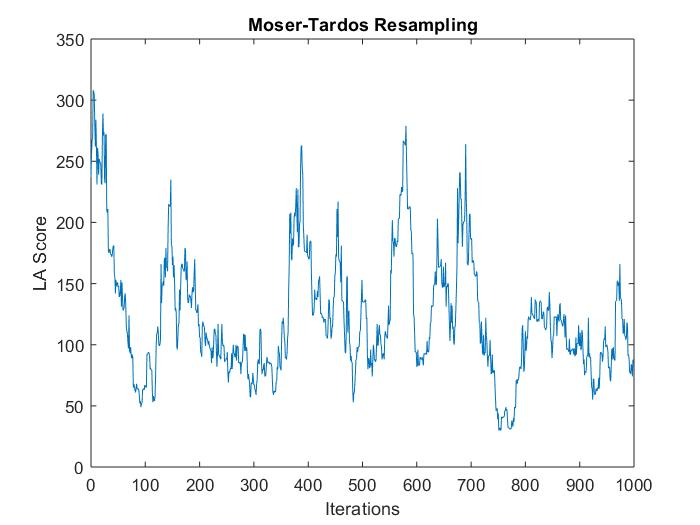
\includegraphics[width=\textwidth,keepaspectratio]{images/pure_random_construction}
\end{figure}

Therefore, in order to construct a valid locating array in this case, one would need to either increase the number of iterations or increase the number of rows in the array.
However, we also consider making a minor change to the approach itself to direct the array towards a valid solution instead of resampling purely at random.
The updated approach is discussed next.

\subsection{Directed Moser-Tardos Resampling} \label{sect:directed}

Figure \ref{fig:construction_pure_mt} shows the array score changing at random to all appearances.
In other words, some changes improve the score, while others worsen the score.
We therefore introduce a new directed construction approach that differs only slightly from Moser-Tardos resampling in that it does not accept any changes that worsen the score of the array.
After every change, the directed approach checks the array score, and if the score worsens, the change is rolled back.
It then resamples randomly repeatedly until it finds a change that does not worsen the array score.
Figure \ref{fig:construction_directed_random} shows the array score through 1000 iterations for the same construction scenario as Figure \ref{fig:construction_pure_mt}.
The score, in this case, decreases sharply and a locating array is successfully constructed after 234 iterations.
Similar to pure Moser-Tardos resampling, however, the directed resampling approach is not guaranteed to finish.

\begin{center}

\begin{figure}[htbp]
\caption{LA score after each iteration using directed Moser-Tardos resampling.}
\label{fig:construction_directed_random}
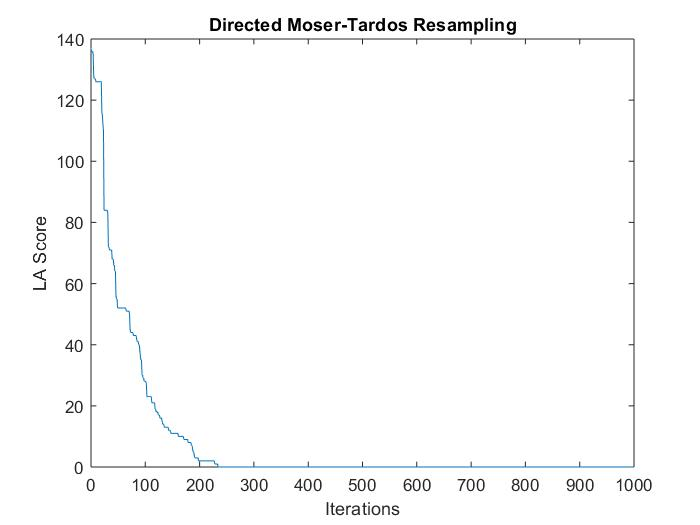
\includegraphics[width=\textwidth,keepaspectratio]{images/directed_random_construction}
\end{figure}

\end{center}

Directed Moser-Tardos resampling can also be easily modified to construct locating arrays with additional constraints such as higher separation.
Only the scoring system must be modified to indicate how close the array is to a valid locating array with a separation value $\delta$.

We modify the scoring approach described in Section \ref{sect:greedy} to score an array, $A$, with a constraint, separation $\delta$, as well.
The modified scoring approach first finds the unique pairs in the compressive sensing matrix, $M$, for $A$, where the separation requirement is violated (the violating pairs).
Then, for every violating pair, the {\em deficiency} of that pair is the number of additional row differences needed for the pair to have $\delta$ row differences.
Following the example in \cite{seidelIWOCA}, if a pair of terms $T_1$, $T_2$ exists where $T_1 \neq T_2$ but $|(\rho(A,T_1) \cup \rho(A,T_2)) \setminus ( \rho(A,T_1) \cap \rho(A,T_2))| = \mu < \delta$, then $T_1$, $T_2$ is a violating pair with deficiency $\delta-\mu$.
The score of $A$ is the same as the total deficiency of $A$ which is the sum of the deficiencies of all violating pairs.
In other words, the score counts the total additonal row differences that all violating pairs collectively need for the separation constraint to be satisfied.
Interestingly, when the only constraint for $A$ is separation $\delta = 1$, then this scoring approach is no different from the one described in Section \ref{sect:greedy}.

An interesting aspect of Algorithm \ref{alg:separation_checker} is that it is easily modified to score the locating array as well as check its validity.
When the fourth terminating condition of the algorithm is satisfied, then the number of pairs with one column in $\mathit{nodeA}$ and the other in $\mathit{nodeB}$ is multiplied by the remaining separation needed, $\delta$.
This is then added to a global variable with the total score which is initialized to zero before the initial call to the checker.
When all recursive calls are completed, the global variable holds the correct total score for a locating array with any separation constraint $\delta$.
Furthermore, this scoring change is implemented with almost no additional runtime cost.

Table \ref{tab:sizes_random} shows factor and level inputs in the first column, and the separation requirements in the second row.
The remainder of the table indicates the size, in terms of rows, needed for directed Moser-Tardos resampling to construct a valid locating array within 1000 iterations, satisfying the separation requirement.

\begin{center}

\begin{table}[htbp]
\caption{Locating array sizes using directed Moser-Tardos resampling.}
\label{tab:sizes_random}
\begin{tabularx}{\textwidth}{|2|2|2|2|2|}
\hline
& \multicolumn{4}{|c|}{Number of Rows} \\
\hline
Type & $\delta=1$ & $\delta=2$ & $\delta=3$ & $\delta=4$ \\
\hline
$2^{10}$        & 14  & 19  & 24  & 30  \\
$2^{15}$        & 17  & 22  & 29  & 34  \\
$2^{20}$        & 19  & 26  & 31  & 37  \\
$2^{50}$        & 26  & 33  & 40  & 47  \\
$2^{75}$        & 28  & 36  & 44  & 50  \\
$2^{100}$       & 31  & 39  & 46  & 53  \\
\hline
$3^{10}$        & 34  & 46  & 57  & 66  \\
$3^{15}$        & 40  & 52  & 65  & 73  \\
$3^{20}$        & 44  & 57  & 69  & 79  \\
$3^{50}$        & 57  & 70  & 83  & 95  \\
$3^{75}$        & 62  & 76  & 90  & 103 \\
$3^{100}$       & 67  & 81  & 94  & 107 \\
\hline
$4^{10}$        & 65  & 86  & 104 & 122 \\
$4^{15}$        & 76  & 96  & 116 & 133 \\
$4^{20}$        & 82  & 104 & 122 & 141 \\
$4^{50}$        & 106 & 129 & 148 & 168 \\
$4^{75}$        & 116 & 138 & 159 & 179 \\
$4^{100}$       & 123 & 146 & 166 & 188 \\
\hline
$5^{10}$        & 110 & 141 & 165 & 194 \\
$5^{15}$        & 126 & 156 & 185 & 212 \\
$5^{20}$        & 138 & 169 & 198 & 225 \\
$5^{50}$        & 173 & 208 & 236 &     \\
$5^{75}$        & 189 & 223 & 256 &     \\
$5^{100}$       & 202 & 235 & 266 &     \\
\hline
$5^{10}2^{10}$  & 110 & 139 & 172 & 197 \\
\hline
\end{tabularx}
\end{table}

\end{center}

Table \ref{tab:sizes_random} was generated using a binary search technique on the locating array size.
We began with an upper bound on the number of rows in the array that easily satisfied all constraints, and a lower bound, an empty array with 0 rows.
A binary search technique was then used to find the smallest possible size for a locating array to be constructed in 1000 iterations under the specified constraints.
In the column under $\delta = 4$, some of the cells are blank because the checker took an extended amount of time in these cases.
Not surprisingly, the locating arrays in Table \ref{tab:sizes_random} with separation $\delta = 1$ produced by directed Moser-Tardos resampling are larger than those shown in Table \ref{tab:sizes_greedy} and produced by Algorithm \ref{alg:greedy_construction} which chooses every row carefully to minimize the array score, and ultimately the final array size.

\section{Summary}

The initial greedy approach presented in Algorithm \ref{alg:greedy_construction} is convenient for creating arrays that satisfy the locating property.
It adds rows as needed, and the only necessary input parameter is factor information.
However, it is unable to construct locating arrays with additional constraints including higher separation.
Instead of modifying Algorithm \ref{alg:greedy_construction} to incorporate separation, we present randomized approaches that can be applied to construct locating arrays with any additional constraints.

Moser-Tardos resampling given in Algorithm \ref{alg:mt_construction} constructs locating arrays with additional constraints.
The main requisite of the algorithm is an efficient checker used repeatedly to check if the array satisfies all requirements.
Additionally, the algorithm requires an input parameter indicating the size of the locating array.

A modification to Moser-Tardos resampling is directed Moser-Tardos resampling discussed in Section \ref{sect:directed}.
As shown in Figure \ref{fig:construction_pure_mt} and Figure \ref{fig:construction_directed_random}, directed Moser-Tardos resampling may construct a locating array in fewer iterations than Moser-Tardos resampling.
However, it requires an additional scoring system to indicate how close the array is to satisfying all requirements.
Finally, we provide Table \ref{tab:sizes_random} to indicate the approximate locating array sizes for several different array types and separation constraints.

\chapter{Analysis} \label{chptr:analysis}

Following the construction of a locating array, the experiments indicated by the array are performed, and results are measured as one or more output variables.
The results must now be analyzed to determine which factors are relevant.
As discussed in Chapter \ref{chptr:introduction}, locating arrays grow logarithmically in the number of factors, making the consideration of an order of magnitude more factors in experimentation practical.
However, to achieve the logarithmic growth rate, locating arrays can be highly unbalanced, and thus new techniques for the analysis of locating arrays are required.

This chapter discusses two existing approaches for analyzing data collected from experimentation based on a locating array introduced in Section \ref{sect:rel_stat_analysis} and Section \ref{sect:rel_dfs_analysis}.
It also describes a new time- and space-efficient analysis technique that is able to support large-scale experimentation and cope with noise in measurements.
The new analysis technique is then used to validate the results from two screening experiments based on locating arrays, one conducted on the \texttt{w-iLab.t} wireless network testbed in Belgium varying 24 factors, and the other conducted in a wireless network simulator varying 75 factors.
Our experimental design and analysis techniques are available for use \cite{mehari2017} in large-scale screening experiments, the first phase of any goal of experimentation.

\section{Analysis Motivation} \label{sect:motivation}

Section \ref{sect:rel_stat_analysis} describes an initial existing analysis technique using a statistical approach.
The approach could be generalized and automated for analysis in other screening experiments, but does not consider alternate explanations for noise in the system.
A second existing analysis technique in Section \ref{sect:rel_dfs_analysis} provides another approach using a depth-first search (DFS) of an explicit tree.
This second approach is general and considers noise, but the algorithm provided is inefficient.
The recursive backjumping employed by the DFS algorithm requires many models and decisions to be tracked which makes memory-efficient implementations difficult.
The DFS algorithm also provides very little control over the runtime of the algorithm.
Our aim is to provide a general, simple, and efficient algorithm for analysis that allows for easy implementation and optimization.

\section{Introducing a New Approach} \label{sect:approach}

We propose a new approach that achieves the same analysis using the same basic "heavy-hitters" method as in existing approaches.
However, the algorithm is novel in that it uses a branch-and-bound approach, conducting the search in a breadth-first manner, storing the tree implicitly in a number of priority queues.
It bounds the number of models in each queue using $R^2$.
Bounds on the number and size of the queues provide parameters to trade running time and space to achieve exploration of a larger portion of the tree. 
Pseudocode for the new branch-and-bound BFS tree-based analysis is given in Algorithm \ref{alg:bfs_analysis}.

Our new approach borrows many ideas from the previous two approaches, but also introduces new ideas in the process.
It uses the same type of "heavy-hitters" algorithm and OMP technique as the existing DFS technique.
However, the approach discussed in Section \ref{sect:rel_dfs_analysis} \cite{Compton-et-al-LA} uses a safety parameter to dictate where to perform back-jumping on the implicit tree.
This parameter helps compare multiple other alternative models that each may contain a different number of terms.
We eliminate this parameter to simplify the process and switch to a BFS approach, eliminating the need to compare alternative models that may each contain a different number of terms.

\begin{algorithm}[pthb]
\caption{$\mathrm{BFS\_Analysis}(\mathit{terms}, M, \mathit{data}, \mathit{nTerms}, \mathit{nNewModels}, \mathit{nModels})$}
\label{alg:bfs_analysis}

\begin{algorithmic}[1]
\REQUIRE List of candidate terms, compressive sensing matrix, vector of performance data, terms per model, number of new models to generate for a particular model, number of models to return
\ENSURE $\mathit{nModels}$ best models with $nTerms$ terms each
\STATE {Initialize $nTerms + 1$ priority queues, each with maximum $\mathit{nModels}$}
\STATE $model_{new} \gets$ [empty model with no terms]
\STATE $residuals_{new} \gets data$
\STATE enqueue($queue_{0},(model_{new},residuals_{new})$)
\FOR{$\ell \gets 0,...,nTerms-1$}
	\WHILE{$queue_{\ell}$ has models}
		\STATE $(model,residuals) \gets $dequeue($queue_{\ell}$)
		\FOR{$i \gets 1,...,nNewModels$}
			\STATE $k \gets$ [$i^{th}$ most significant term from $M$]
			\STATE $model_{new} \gets \mathrm{LS}(terms(model) \cup [terms_k],data)$
			\STATE $residuals_{new} \gets residuals - model_{new}$
			\STATE enqueue($queue_{\ell+1},(model_{new},residuals_{new})$)
		\ENDFOR
	\ENDWHILE
\ENDFOR
\RETURN $queue_{nTerms}$
\end{algorithmic}
\end{algorithm}

Ultimately, the new BFS tree analysis algorithm attempts to find the models with the highest $R^2$ values, each with $nTerms$ terms, in a straightforward manner.
It starts by initializing the zeroth priority queue to hold the empty model with $R^2 = 0$. 
The algorithm then removes the model from the zeroth priority queue, and generates $nNewModels$ models, each with one term from the most significant terms of the compressive sensing matrix, $M$, selected by OMP. 
This differs from the DFS tree algorithm by considering multiple models rather than exploring a single model at a time.
Least squares is run on each of these models to obtain their $R^2$ values, and they are then placed in the first priority queue, ranked by $R^2$. 

The process is repeated on the first priority queue to generate new models, each with two terms, that are added to the second priority queue. 
Each queue only stores the best models by $R^2$ up to its bound, $nModels$.
If a queue is full, then an attempt to enqueue a model with $R^2$ lower than the model with the lowest $R^2$ does not succeed.
Similarly, an attempt to enqueue a model with $R^2$ greater than the model with the lowest $R^2$ evicts that model from the queue. 
The process is repeated until the final priority queue contains $nModels$ models each with $nTerms$ terms.
 
The parameters of the BFS tree algorithm, $nModels$, $nNewModels$, and $nTerms$ can be adjusted as desired.
Higher values of $nNewModels$ result in more models fit using least squares, thus increasing execution time, but also increasing the likelihood that the models with the best $R^2$ values are found. 
Lower values of $nNewModels$ result in fewer models fit, decreasing execution time but possibly resulting in models with lower $R^2$ values found.
Similarly, higher values of $nModels$ lead to a larger bound on the number of models stored and analyzed, increasing execution time. 
Lower values of $nModels$ risk discarding a model that might become much better, with respect to $R^2$, when more terms are added.
Finally, the parameter $nTerms$ must be chosen carefully to propery fit the model.
When $nTerms$ is too small, the analysis does not find all terms relevant to the system and produces poor models, and when $nTerms$ is too large, the analysis overfits the models.
In Chapter \ref{chptr:conclusion}, we discuss choosing $nModels$, $nNewModels$, and $nTerms$ dynamically in future work.

Another issue that must be accounted for is that of duplicate models. 
It is possible that multiple models with identical terms, but in different orders, are added to the same priority queue. 
%For example, consider two models added to the first priority queue, one with term $A$ and the other with term $B$. 
%Suppose again that the model with term $A$ has term $B$ added to it, and that the model with term $B$ has term $A$ added to it. 
%If both models are added to the second priority queue there are two models with the same terms. 
The algorithm must discard such duplicate models. % when their $R^2$ values are identical.

When the algorithm completes, the final priority queue holds, at most, the number of models given by $nModels$. 
These models are ordered by $R^2$ and given as the best models each with $nTerms$ terms.

The execution time and memory usage of Algorithm \ref{alg:bfs_analysis} can be easily adjusted using the parameters $nModels$, $nNewModels$, and $nTerms$.
Our approach iterates through $nTerms$ priority queues, extracts $nModels$ from each, finds the best terms using OMP dictated by $nNewModels$, and performs least squares after adding each term. 
Assuming least squares takes, in the worst case, time $nTerms$, the execution time for this algorithm is $O( \mathit{nTerms}^{2} \cdot \mathit{nModels} \cdot \mathit{nNewModels} )$. 
This approach also considers one priority queue at a time, each with size $nModels$. 
Assuming each model takes constant space, the memory usage is $O(nModels)$. 

In screening, we are interested in identifying the most significant factors and two-way interactions impacting performance.
One way to determine the screening results is to examine occurrences of the factors in these models and select those occurring most often.
We discuss this next.

\section{Counting Occurrences} \label{sect:occurrences}

The new BFS analysis approach produces and returns the top $\mathit{nModels}$ models.
In the top models generated, many factors are included multiple times in multiple models.
We count the occurrences of each factor in the top $\mathit{nModels}$ models, and rank the factors by number of occurrences.
Because terms in a model can be interactions between factors, or a factor can appear with different levels, the same factor may occur multiple times in the same model. 
A factor {\em occurrence} is defined as any time a factor appears in a model, no matter its level, or if it is part of an interaction.
An interaction {\em occurrence} is defined as any time a pair of factors appear in a model as an interaction, no matter the level of either factor. 
In the following section, we rank all factors by how often they occur in the top $\mathit{nModels}$ models.
Interactions are also examined but with a separate ranking.
We hypothesize that a significant factor occurs frequently in the top models and is therefore highly ranked, while an insignificant factor rarely appears in the ranking, if at all.

\section{Validation} \label{sect:validation}

We compare our BFS tree algorithm to the DFS tree algorithm in \cite{Compton-et-al-LA}.
We use a C++ implementation to generate the top 50 models, with 11 terms each, using our BFS tree algorithm for both voice quality and RF exposure. 
Finally, we count the occurrences of each factor in the top 50 models and rank all factors by the number of occurrences. 
We use the same testbed data collected and used in \cite{Compton-et-al-LA}.
The full-factorial design for this factor space has over $10^{13}$ tests while the locating array has only 109 tests.

Table \ref{tab:validate-mos} shows the factors ranked by the number of occurrences in our BFS tree results for the voice quality performance metric.
The table also indicates the factors selected by the DFS algorithm \cite{Compton-et-al-LA}.
Three of the four significant factors for voice quality listed in \cite{Compton-et-al-LA} are the top three factors in our BFS tree results. 
This indicates a strong correspondence between the output of the DFS and BFS algorithms with the difference likely due to the DFS algorithm exploring a different, or smaller, portion of the search tree since it stops after generating 1024 models.
This also likely accounts for the BFS algorithm not agreeing with the fourth significant factor.

\begin{table}
\caption{Significant factors impacting voice quality from data collected from the \texttt{w-iLab.t} testbed.}
\label{tab:validate-mos}

\begin{tabularx}{\textwidth}{|2|7|1|}
\hline
\multicolumn{3}{|c|}{\textbf{BFS Occurrence Counts}} \\
\hline
Count & Factor & In \cite{Compton-et-al-LA} \\
\hline
150	& $\mathit{intCOR}$					& $\surd$ \\
136	& $\mathit{band}$					& $\surd$ \\
133	& $\mathit{txpower}$				& $\surd$ \\
100	& $\mathit{sensing}$				& \\
 71	& $\mathit{rate}$					& \\
 48	& $\mathit{udp\_mem\_pressure}$		& \\
 48	& $\mathit{ipfrag\_low\_thresh}$	& \\
 34	& $\mathit{wmem\_max}$				& \\
 22	& $\mathit{codecBitrate}$			& $\surd$ \\
 16	& $\mathit{txqueuelen}$				& \\
 15	& $\mathit{mtu}$					& \\
 14	& $\mathit{channel}$				& \\
 12	& $\mathit{frameLen}$				& \\
  9	& $\mathit{wmem\_default}$			& \\
  7	& $\mathit{ROHC}$					& \\
  6	& $\mathit{codec}$					& \\
  5	& $\mathit{ipfrag\_high\_thresh}$	& \\
  5	& $\mathit{udp\_wmem\_min}$			& \\
  4	& $\mathit{udp\_rmem\_min}$			& \\
  3	& $\mathit{rmem\_max}$				& \\
  3	& $\mathit{qdisc}$					& \\
  1	& $\mathit{rmem\_default}$			& \\
  1	& $\mathit{udp\_mem\_min}$			& \\
  \hline
\end{tabularx}

\end{table}

Interestingly, our BFS tree analysis identified some potential two-way interactions for voice quality that the DFS tree analysis did not identify.
Table \ref{tab:2way-mos} shows the top interactions; in this case, they exhibit strong heredity.

\begin{table}
\caption{Significant two-way interactions impacting voice quality from data collected from \texttt{w-iLab.t}.}
\label{tab:2way-mos}

\begin{tabularx}{\textwidth}{|2|8|}
\hline
\multicolumn{2}{|c|}{\textbf{BFS Occurrence Counts}} \\
\hline
Count & Interaction \\
\hline
 51	& $\mathit{intCOR}$ \& $\mathit{band}$ \\
 49	& $\mathit{intCOR}$ \& $\mathit{sensing}$ \\
 49	& $\mathit{sensing}$ \& $\mathit{band}$ \\
 48	& $\mathit{udp\_mem\_pressure}$ \& $\mathit{ipfrag\_low\_thresh}$ \\
 33	& $\mathit{rate}$ \& $\mathit{band}$ \\
 30	& $\mathit{rate}$ \& $\mathit{wmem\_max}$ \\
 11	& $\mathit{txqueuelen}$ \& $\mathit{frameLen}$ \\
  9	& $\mathit{txpower}$ \& $\mathit{channel}$ \\
  9	& $\mathit{wmem\_default}$ \& $\mathit{codecBitrate}$ \\
  8	& $\mathit{mtu}$ \& $\mathit{txpower}$ \\
\hline
\end{tabularx}

\end{table}

Table \ref{tab:validate-exp} shows the factors ranked by the number of occurrences in our BFS tree results for the RF exposure performance metric. 
For exposure, five of the top six factors match in the two algorithms.
The largest number of occurrences of any two-way interaction for exposure was only six, so we do not consider any interaction to be significant.

\begin{table}[h]
\caption{Significant factors impacting RF exposure from data collected from the \texttt{w-iLab.t} testbed.}
\label{tab:validate-exp}

\begin{tabularx}{\textwidth}{|2|7|1|}
\hline
\multicolumn{3}{|c|}{\textbf{BFS Occurrence Counts}} \\
\hline
Count & Factor & In \cite{Compton-et-al-LA} \\
\hline
156	& $\mathit{rate}$					& $\surd$ \\
152	& $\mathit{txpower}$				& $\surd$ \\
 98	& $\mathit{codecBitrate}$			& $\surd$ \\
 60	& $\mathit{frameLen}$				& $\surd$ \\
 56	& $\mathit{band}$					& $\surd$ \\
  4	& $\mathit{codec}$					& \\
  4	& $\mathit{ROHC}$					& \\
  2	& $\mathit{wmem\_max}$				& \\
  2	& $\mathit{ipfrag\_low\_thresh}$	& \\
  2	& $\mathit{udp\_mem\_min}$			& \\
  2	& $\mathit{qdisc}$					& \\
  2	& $\mathit{channel}$				& \\
\hline
\end{tabularx}

\end{table}

The factors screened as significant are plausible. 
For example, one would expect that transmission power ($\mathit{txpower}$) should have an effect on both exposure and audio quality, and that interference should have an effect on audio quality but not exposure.

Our comparisons show a strong correspondence to the results obtained from the DFS tree algorithm in \cite{Compton-et-al-LA} and our BFS tree algorithm therefore validates the screening analysis in \cite{Compton-et-al-LA}. 
In addition, our new approach is more memory efficient and provides parameters to control runtime.
Indeed, the BFS tree algorithm is able to analyze the even larger-scale data collected from experimentation in simulation described next, where the DFS tree algorithm was unable to complete the analysis because of memory constraints.

In \cite{AldacoCS15}, 75 factors of the protocols spanning the MAC to the transport layer, as well as the wireless environment and the simulation environment, having from two to ten values each, were screened in a simulation model of a mobile wireless network.
The goal was to determine the significant factors and two-way interactions impacting TCP throughput.
The full-factorial design for this factor space is even larger than the testbed experiment; it has over $10^{43}$ tests in the array! 
In contrast, the locating array has only 421 tests.

Aldaco et al.\ \cite{AldacoCS15} perform screening analysis on the data collected from simulation using the method described in Section \ref{sect:rel_stat_analysis}.
A model with 13 terms having 9 unique factors are identified as significant.
We use our BFS tree algorithm to perform screening analysis on the same data set. 
The parameters for our algorithm were set to produce 50 models, each with 13 terms; these models differed very little in $R^2$ values. 

We again counted the occurrences of each factor in the top 50 models and ranked all factors by the number of occurrences. 
Table \ref{tab:tput-sim} shows the resulting ranking and an indicator when the factor is also identified as significant in \cite{AldacoCS15}. 
Interestingly, the top eight factors, by number of occurrences, are also factors identified by Aldaco et al.\ \cite{AldacoCS15} as significant. 
Therefore, eight of the nine factors identified by Aldaco et al.\ were the top eight factors identified by the BFS tree algorithm. 
We also counted the occurrences of interactions between two factors and ranked all interactions by the number of occurrences. 
%Even though our analysis includes the levels in the interactions it finds, we did not include them in our occurrences ranking for simplicity. 

Table \ref{tab:inter-sim} shows the interactions ranked by the number of occurrences in the BFS tree results and an indicator when the interaction is also identified in \cite{AldacoCS15} as significant. 
Interestingly, three of the top four interactions, by number of occurrences, were also interactions identified by Aldaco et al.\ as significant.
However, Aldaco et al.\ did identify a fourth interaction that was not found by the BFS tree algorithm. 

\begin{table}
\centering
\caption{Significant factors impacting TCP throughput from data collected from a wireless network simulation.}
\label{tab:tput-sim}

\begin{tabularx}{\textwidth}{|2|7|1|}
\hline
\multicolumn{3}{|c|}{\textbf{BFS Occurrence Counts}} \\
\hline
Count & Factor & In \cite{AldacoCS15} \\
\hline
148	& $\mathit{MAC\_RTSThreshold}$			& $\surd$ \\
142	& $\mathit{ErrorModel\_unit}$			& $\surd$ \\
100	& $\mathit{TCP\_packetSize}$			& $\surd$ \\
100	& $\mathit{TCP\_min\_RTO}$				& $\surd$ \\
100	& $\mathit{ErrorModel\_ranvar}$			& $\surd$ \\
 98	& $\mathit{RWP\_Area}$					& $\surd$ \\
 53	& $\mathit{ErrorModel\_rate}$			& $\surd$ \\
 50	& $\mathit{ARP\_flows}$					& $\surd$ \\
 27	& $\mathit{Propagation}$				& \\
 26	& $\mathit{DSSS\_CWMin\_CWMax}$			& \\
 25	& $\mathit{TCP\_slow\_start\_restart}$	& \\
 16	& $\mathit{TCP\_RTTvar\_exp}$			& $\surd$ \\
 15	& $\mathit{TCP\_maxburst}$				& \\
 13	& $\mathit{Queue\_acksfirst}$			& \\
 12	& $\mathit{AODV\_TTL\_START}$			& \\
  8	& $\mathit{ENER\_initialEnergy}$		& \\
  8	& $\mathit{MAC\_ProbeDelay}$			& \\
  8	& $\mathit{TCP\_updated\_rttvar}$		& \\
  5	& $\mathit{TCP\_numdupacksFrac}$		& \\
  3	& $\mathit{AODV\_HELLO\_INTERVAL}$		& \\
  3	& $\mathit{TCP\_decrease\_num}$			& \\
  3	& $\mathit{MAC\_ScanType}$				& \\
  3	& $\mathit{Queue\_DT\_queue\_in\_bytes}$	& \\
  3	& $\mathit{Queue\_interleave}$			& \\
  2	& $\mathit{Queue\_ackfromfront}$		& \\
  2	& $\mathit{TCP\_rttvar\_init}$			& \\
  1	& $\mathit{Queue\_DT\_summarystats}$	& \\
  1	& $\mathit{TCP\_TRTTVAR\_BITS}$			& \\
\hline
\end{tabularx}

\end{table}

\begin{table}
\centering
\caption{Significant two-way interactions impacting TCP throughput in a wireless network simulation.}
\label{tab:inter-sim}

\begin{tabularx}{\textwidth}{|2|7|1|}
\hline
\multicolumn{3}{|c|}{\textbf{BFS Occurrence Counts}} \\
\hline
Count & Interaction & In \cite{AldacoCS15} \\
\hline
56	& $\mathit{RWP\_Area}$ \& $\mathit{MAC\_RTSThreshold}$				& \\
50	& $\mathit{ErrorModel\_rate}$ \& $\mathit{ErrorModel\_unit}$		& $\surd$ \\
50	& $\mathit{MAC\_RTSThreshold}$ \& $\mathit{ErrorModel\_ranvar}$		& $\surd$ \\
50	& $\mathit{ErrorModel\_unit}$ \& $\mathit{ErrorModel\_ranvar}$		& $\surd$ \\
42	& $\mathit{MAC\_RTSThreshold}$ \& $\mathit{ErrorModel\_unit}$		& \\
26	& $\mathit{DSSS\_CWMin\_CWMax}$ \& $\mathit{Propagation}$			& \\
16	& $\mathit{TCP\_min\_RTO}$ \& $\mathit{TCP\_slow\_start\_restart}$	& \\
14	& $\mathit{TCP\_maxburst}$ \& $\mathit{TCP\_RTTvar\_exp}$			& \\
8	& $\mathit{ARP\_flows}$ \& $\mathit{TCP\_slow\_start\_restart}$		& \\
8	& $\mathit{RWP\_Area}$ \& $\mathit{Queue\_acksfirst}$				& \\
\hline
\end{tabularx}

\end{table}

Again, our comparisons show a strong correspondence to the results presented in Aldaco et al.\ \cite{AldacoCS15}.
It is therefore reasonable to conclude that our BFS tree analysis algorithm successfully identifies those factors and two-way interactions, that are most significant to the TCP throughput of the mobile wireless network.
It is also reasonable to conclude that counting occurrences is a valid approach for determining what factors are most significant from the top $\mathit{nModels}$.
A better approach than counting occurrences may exist but we leave this problem for future work in Chapter \ref{chptr:conclusion}.

\section{Summary}

Algorithm \ref{alg:bfs_analysis} is a simple, general, and efficient analysis approach for the output measurements from locating arrays.
The algorithm can be used to analyze any locating array with its corresponding output measurements to find significant factors and interactions.
It uses three input parameters that control how many models are stored, how many alternative models to check, and how many terms to add to each model.
These parameters are currently static throughout the analysis execution.
Future work includes the possibility of modifying these parameters to be dynamic.
Furthermore, the algorithm assumes that the significant system factors and interactions follow a "heavy-hitters" pattern.
The next chapter investigates this assumption and how the algorithm behaves when the system does not follow this pattern.

\chapter{Robustness} \label{chptr:robustness}

During the discussion of our new analysis technique in Section \ref{sect:approach}, an assumption was made that the system factors must follow a "heavy-hitters" pattern.
We also did not discuss how noise might affect our analysis technique, although noise is always present in real-world applications and often introduced in simulated systems.
In this chapter, we discuss "heavy-hitters" and see how robust our analysis is when the assumption is violated.
We also discuss the effects of noise in the system on the analysis algorithm.
Chapter \ref{chptr:construction} introduces separation and hypothesizes that higher separation leads to more accurate results in analysis.
This chapter investigates how separation might help, particularly when a large amount of noise is introduced.
Finally, Section \ref{sect:interesting} discusses an interesting phenomenon that was coincidentally discovered when investigating the effects of noise.

\section{"Heavy-Hitters" Requirement} \label{sect:heavyhitters}

In Chapter \ref{chptr:analysis}, we discussed how our analysis algorithm assumes a "heavy-hitters" scenario.
We call this the "heavy-hitters" requirement.
The analysis is thus a method that relies on the assumption that there is one term, a main effect or interaction, that affects the output more significantly than all remaining terms, and when this significant term is removed, there again exists one main effect or interaction that affects the output more significantly than all remaining terms.
In other words, the significance of the factors and interactions follows an exponentially decreasing pattern that allows them to be easily identified, one by one, over all other terms.
In this section, we begin with a simple example of when the "heavy-hitters" requirement is satisfied, and when it is not.
We then move on to more complex examples.

Suppose the true model for a system is given in Table \ref{tab:scenario_1a}.
This means that the output of the system is determined by the specific terms listed, along with their coefficients, i.e., the output is a function of the form $a \cdot T_{3} + b \cdot T_{4} + c \cdot \mathit{INTERCEPT}$.
We then attempt to use our analysis algorithm to recover the true terms of the model using only the output of the system.
A partial CS matrix along with the output (responses) of the system are also given in Table \ref{tab:scenario_1a}.

\begin{table}
\caption{Robustness Scenario 1A - Without Heavy-Hitters}
\label{tab:scenario_1a}

\begin{tabularx}{\textwidth}{|2|8|}
\hline
\multicolumn{2}{|c|}{True Model - Does not satisfy "heavy-hitters"} \\
\hline
Coefficient & Term \\
\hline
1 & $\mathit{INTERCEPT}$ \\
1 & $T_{3}$ \\
1 & $T_{4}$ \\
\hline
\end{tabularx}

\begin{tabularx}{\textwidth}{|2|1|1|1|1||4|}
\hline
\multicolumn{6}{|c|}{Partial CS Matrix and Responses} \\
\hline
$\mathit{INTERCEPT}$ & $T_{1}$ & $T_{2}$ & $T_{3}$ & $T_{4}$ & Response \\
\hline
 1      & 1   & -1  & -1  & -1  & 1        \\
 1      & -1  & 1   & -1  & -1  & 1        \\
 1      & -1  & -1  & 1   & -1  & -1       \\
 1      & -1  & -1  & -1  & 1   & -1       \\
\hline
\end{tabularx}
\end{table}

A trace of the analysis using Algorithm \ref{alg:bfs_analysis} proceeds:

\begin{enumerate}  
\item The algorithm begins with a model consisting of only the intercept which is the average of all output values:
	\[
		0 \cdot \mathit{INTERCEPT}
	\]
\item The residuals are:
	\[
		{\begin{bmatrix} 1 & 1 & -1 & -1 \end{bmatrix}}^T
	\]
\item Absolute dot products calculated for $T_{1}$ to $T_{4}$ are:
	\[
		2, 2, 2, 2
	\]
\item Because all absolute dot products are the same, any term may be added depending on noise.
	Suppose the first term, $T_{1}$, is added.
\item Least squares is now run and the model becomes:
	\[
		\frac{1}{3} \cdot \mathit{INTERCEPT} + \frac{2}{3} \cdot T_{1}
	\]
\item The residuals are:
	\[
		{\begin{bmatrix} 0 & \frac{4}{3} & -\frac{2}{3} & -\frac{2}{3} \end{bmatrix}}^T
	\]
\item Absolute dot products calculated for $T_{2}$ to $T_{4}$ are:
	\[
		\frac{8}{3}, \frac{4}{3}, \frac{4}{3}
	\]
\item $T_{2}$ has the largest absolute dot product and it is added to the model.
\item Least squares is now run and the model becomes:
	\[
		1 \cdot \mathit{INTERCEPT} + 1 \cdot T_{1} + 1 \cdot T_{2}
	\]
\item The residuals are:
	\[
		{\begin{bmatrix} 0 & 0 & 0 & 0 \end{bmatrix}}^T
	\]
\end{enumerate}

The analysis using Algorithm \ref{alg:bfs_analysis} stops because it has now explained the response completely.
However, the terms in the model recovered do not equal the terms in the true model listed in Table \ref{tab:scenario_1a}.
This is because the coefficients are all so close together that they can easily hide each other's effects.
Suppose now we use the true model in Table \ref{tab:scenario_1b} which satisfies the "heavy-hitters" requirement with the same experiments.

\begin{table}
\caption{Robustness Scenario 1B - With Heavy-Hitters}
\label{tab:scenario_1b}

\begin{tabularx}{\textwidth}{|2|8|}
\hline
\multicolumn{2}{|c|}{True Model - Does satisfy "heavy-hitters"} \\
\hline
Coefficient & Term \\
\hline
1 & $\mathit{INTERCEPT}$ \\
4 & $T_{3}$ \\
10 & $T_{4}$ \\
\hline
\end{tabularx}

\begin{tabularx}{\textwidth}{|2|1|1|1|1||4|}
\hline
\multicolumn{6}{|c|}{Partial CS Matrix and Responses} \\
\hline
$\mathit{INTERCEPT}$ & $T_{1}$ & $T_{2}$ & $T_{3}$ & $T_{4}$ & Response \\
\hline
 1      & 1   & -1  & -1  & -1  & -13      \\
 1      & -1  & 1   & -1  & -1  & -13      \\
 1      & -1  & -1  & 1   & -1  & -5       \\
 1      & -1  & -1  & -1  & 1   & 7        \\
\hline
\end{tabularx}

\end{table}

A trace of the analysis using Algorithm \ref{alg:bfs_analysis} proceeds:

\begin{enumerate}
\item The algorithm begins with a model consisting of only the intercept which is the average of all output values:
	\[
		-6 \cdot \mathit{INTERCEPT}
	\]
\item The residuals are:
	\[
		{\begin{bmatrix} -7 & -7 & 1 & 13 \end{bmatrix}}^T
	\]
\item Absolute dot products calculated for $T_{1}$ to $T_{4}$ are:
	\[
		14, 14, 2, 26
	\]
\item $T_{4}$ has the largest absolute dot product and it is added to the model.
\item Least squares is now run and the model becomes:
	\[
		-\frac{5}{3} \cdot \mathit{INTERCEPT} + \frac{26}{3} \cdot T_{4}
	\]
\item The residuals are:
	\[
		{\begin{bmatrix} -\frac{8}{3} & \frac{8}{3} & \frac{16}{3} & 0 \end{bmatrix}}^T
	\]
\item Absolute dot products calculated for $T_{1}$ to $T_{3}$ are:
	\[
		\frac{16}{3}, \frac{16}{3}, \frac{32}{3}
	\]
\item $T_{3}$ has the largest absolute dot product and it is added to the model.
\item Least squares is now run and the model becomes:
	\[
		1 \cdot \mathit{INTERCEPT} + 4 \cdot T_{3} + 10 \cdot T_{4}
	\]
\item The residuals are:
	\[
		{\begin{bmatrix} 0 & 0 & 0 & 0 \end{bmatrix}}^T
	\]
\end{enumerate}

The analysis using Algorithm \ref{alg:bfs_analysis} has now explained the response completely, and it has recovered the same terms as the true model listed in Table \ref{tab:scenario_1b}.
Table \ref{tab:scenario_1a} illustrates how failure to meet the "heavy-hitters" requirement can lead to the recovery of models that appear good, but are not the actual model.
Table \ref{tab:scenario_1b} then shows how meeting the "heavy-hitters" requirement can lead to the recovery of the actual model.
However, these scenarios are extremely basic, and we now turn to more interesting and realistic examples.
We use a systematic study on synthetic data because the limitations of our recovery must be understood.
In real systems, the function we are trying to recover is unknown.

In our more complex examples, we first create a locating array for a set of factors and their levels.
Next, we create a model with a set of main effects or interactions.
Artificial experimental output measurements are then generated using the chosen true model.
The output measurements are initially generated without any noise.
Finally, we run our analysis software with the constructed locating array and the measured responses, and evaluate how well the analysis can recover the chosen true model.

Suppose we are interested in a screening experiment with 100 factors, $F_{1}, F_{2}, \dots, F_{100}$.
Each of these factors can be set to 3 levels, $v_1, v_2, v_3$.
Significant terms can be main effects or interactions.
The locating array constructed with separation parameter $\delta=1$ has just 70 rows.
This locating array is used in the sequel unless specified otherwise.

Consider the scenario with the true network model in Table \ref{tab:scenario_2a}.
The true system model is shown at the top of the table, and includes main effects as well as interactions which are indicated by two main effects separated by an ampersand.
The parameters for the analysis algorithm are provided just below the true system model.
Finally, the occurrence counts are shown at the bottom, and the checkmarks in the last column indicate the factors that can also be found in the true model.
The "heavy-hitters" requirement indicates that the coefficients should follow an exponentially decreasing pattern, but it is clear that the true model completely fails to satisfy this.
In fact, every single term carries the same coefficient, 0.1, and the coefficients exhibit 0\% decrease between them.
Yet the analysis found all nine factors in the true model and placed them first.
However, the four factors ranked six through nine have occurrence counts that are less than 50 indicating that these factors did not appear in every model.
Therefore, although it ranked them first, the true factors were not included in all of the generated models.

\begin{table}
\caption{Robustness Scenario 2A - Heavy-Hitters (0\% Decrease)}
\label{tab:scenario_2a}

\begin{tabularx}{\textwidth}{|2|8|}
\hline
\multicolumn{2}{|c|}{True Model - Coefficients exhibit 0\% decrease} \\
\hline
Coefficient & Term \\
\hline
0.1 & $F_{29}=v_1$ \\
0.1 & $F_{98}=v_3$ \& $F_{34}=v_2$ \\
0.1 & $F_{50}=v_2$ \\
0.1 & $F_{22}=v_1$ \\
0.1 & $\mathit{INTERCEPT}$ \\
0.1 & $F_{69}=v_1$ \& $F_{23}=v_1$ \\
0.1 & $F_{10}=v_2$ \\
0.1 & $F_{82}=v_1$ \\
\hline
\end{tabularx}

\begin{tabularx}{\textwidth}{|3|4|3|}
\hline
\multicolumn{3}{|c|}{Analysis Parameters} \\
\hline
$nModels=50$ & $nNewModels=50$ & $nTerms=8$ \\
\hline
\end{tabularx}

\begin{tabularx}{\textwidth}{|1|1|7|1|}
\hline
\multicolumn{4}{|c|}{Occurrence Counts} \\
\hline
Rank & Count & Factor & True \\
\hline
 1 & 50 & $F_{82}$ & $\surd$ \\
 2 & 50 & $F_{50}$ & $\surd$ \\
 3 & 50 & $F_{29}$ & $\surd$ \\
 4 & 50 & $F_{22}$ & $\surd$ \\
 5 & 50 & $F_{10}$ & $\surd$ \\
 6 & 38 & $F_{23}$ & $\surd$ \\
 7 & 35 & $F_{34}$ & $\surd$ \\
 8 & 34 & $F_{98}$ & $\surd$ \\
 9 & 30 & $F_{69}$ & $\surd$ \\
10 &  6 & $F_{6}$  & \\
\hline
\end{tabularx}

\end{table}

The scenario in Table \ref{tab:scenario_2b} uses a true system model in which coefficients decrease by approximately 9\%.
The true model is now closer to satisfying the "heavy-hitters" requirement as the term coefficients are no longer the same.
Again, the analysis found all nine factors in the true model and placed them first.
Of those, only the factors ranked eight and nine have occurrence counts that are less than 50.
This means that only two of the true factors were not found in all of the generated models.
This is an improvement over the previous scenario.
The last two factors on the occurrence count list are $F_{23}$ and $F_{69}$.
These factors are only found in one interaction with a small coefficient (0.12) in the true model.
Hence it is not surprising that they were listed last.

\begin{table}
\caption{Robustness Scenario 2B - Heavy-Hitters (9\% Decrease)}
\label{tab:scenario_2b}

\begin{tabularx}{\textwidth}{|2|8|}
\hline
\multicolumn{2}{|c|}{True Model - Coefficients exhibit 9\% decrease} \\
\hline
Coefficient & Term \\
\hline
0.19 & $F_{29}=v_1$ \\
0.18 & $F_{98}=v_3$ \& $F_{34}=v_2$ \\
0.16 & $F_{50}=v_2$ \\
0.15 & $F_{22}=v_1$ \\
0.13 & $\mathit{INTERCEPT}$ \\
0.12 & $F_{69}=v_1$ \& $F_{23}=v_1$ \\
0.11 & $F_{10}=v_2$ \\
0.1  & $F_{82}=v_1$ \\
\hline
\end{tabularx}

\begin{tabularx}{\textwidth}{|3|4|3|}
\hline
\multicolumn{3}{|c|}{Analysis Parameters} \\
\hline
$nModels=50$ & $nNewModels=50$ & $nTerms=8$ \\
\hline
\end{tabularx}

\begin{tabularx}{\textwidth}{|1|1|7|1|}
\hline
\multicolumn{4}{|c|}{Occurrence Counts} \\
\hline
Rank & Count & Factor & True \\
\hline
 1 & 50 & $F_{98}$ & $\surd$ \\
 2 & 50 & $F_{82}$ & $\surd$ \\
 3 & 50 & $F_{50}$ & $\surd$ \\
 4 & 50 & $F_{34}$ & $\surd$ \\
 5 & 50 & $F_{29}$ & $\surd$ \\
 6 & 50 & $F_{22}$ & $\surd$ \\
 7 & 50 & $F_{10}$ & $\surd$ \\
 8 & 23 & $F_{23}$ & $\surd$ \\
 9 & 13 & $F_{69}$ & $\surd$ \\
10 & 10 & $F_{2}$  & \\
\hline
\end{tabularx}

\end{table}

The scenario in Table \ref{tab:scenario_2c} brings the true model even closer to satisfying the "heavy-hitters" requirement.
All coefficients decrease by 33\%.
Furthermore, the analysis now not only finds all nine factors in the true model, but all significant factors are now found 50 times, and the tenth factor listed is found only twice.
This is an extremely sharp drop-off and delineates the nine significant factors from the tenth insignificant factor.
Such a table of occurrence counts appears useful for screening.

\begin{table}
\caption{Robustness Scenario 2C - Heavy-Hitters (33\% Decrease)}
\label{tab:scenario_2c}

\begin{tabularx}{\textwidth}{|2|8|}
\hline
\multicolumn{2}{|c|}{True Model - Coefficients exhibit 33\% decrease} \\
\hline
Coefficient & Term \\
\hline
1.71 & $F_{29}=v_1$ \\
1.14 & $F_{98}=v_3$ \& $F_{34}=v_2$ \\
0.76 & $F_{50}=v_2$ \\
0.51 & $F_{22}=v_1$ \\
0.34 & $\mathit{INTERCEPT}$ \\
0.23 & $F_{69}=v_1$ \& $F_{23}=v_1$ \\
0.15 & $F_{10}=v_2$ \\
0.1  & $F_{82}=v_1$ \\
\hline
\end{tabularx}

\begin{tabularx}{\textwidth}{|3|4|3|}
\hline
\multicolumn{3}{|c|}{Analysis Parameters} \\
\hline
$nModels=50$ & $nNewModels=50$ & $nTerms=8$ \\
\hline
\end{tabularx}

\begin{tabularx}{\textwidth}{|1|1|7|1|}
\hline
\multicolumn{4}{|c|}{Occurrence Counts} \\
\hline
Rank & Count & Factor & True \\
\hline
 1 & 51 & $F_{69}$ & $\surd$ \\
 2 & 51 & $F_{50}$ & $\surd$ \\
 3 & 51 & $F_{34}$ & $\surd$ \\
 4 & 51 & $F_{23}$ & $\surd$ \\
 5 & 51 & $F_{22}$ & $\surd$ \\
 6 & 51 & $F_{10}$ & $\surd$ \\
 7 & 50 & $F_{98}$ & $\surd$ \\
 8 & 50 & $F_{82}$ & $\surd$ \\
 9 & 50 & $F_{29}$ & $\surd$ \\
10 & 2  & $F_{99}$ & \\
\hline
\end{tabularx}

\end{table}

The next section (\ref{sect:noise}) explores how noise affects occurrence counts, and we explore scenarios that satisfy the "heavy-hitters" requirement even more strongly.
For the sake of completeness, however, and because we contrast against them in the next section, we provide here two more scenarios in Table \ref{tab:scenario_2d} and Table \ref{tab:scenario_2e}.
The scenario in Table \ref{tab:scenario_2d} changes the coefficients to decrease by 50\%, and the coefficients in Table \ref{tab:scenario_2e} exhibit a 60\% decrease.

\begin{table}
\caption{Robustness Scenario 2D - Heavy-Hitters (50\% Decrease)}
\label{tab:scenario_2d}

\begin{tabularx}{\textwidth}{|2|8|}
\hline
\multicolumn{2}{|c|}{True Model - Coefficients exhibit 50\% decrease} \\
\hline
Coefficient & Term \\
\hline
12.8 & $F_{29}=v_1$ \\
6.4  & $F_{98}=v_3$ \& $F_{34}=v_2$ \\
3.2  & $F_{50}=v_2$ \\
1.6  & $F_{22}=v_1$ \\
0.8  & $\mathit{INTERCEPT}$ \\
0.4  & $F_{69}=v_1$ \& $F_{23}=v_1$ \\
0.2  & $F_{10}=v_2$ \\
0.1  & $F_{82}=v_1$ \\
\hline
\end{tabularx}

\begin{tabularx}{\textwidth}{|3|4|3|}
\hline
\multicolumn{3}{|c|}{Analysis Parameters} \\
\hline
$nModels=50$ & $nNewModels=50$ & $nTerms=8$ \\
\hline
\end{tabularx}

\begin{tabularx}{\textwidth}{|1|1|7|1|}
\hline
\multicolumn{4}{|c|}{Occurrence Counts} \\
\hline
Rank & Count & Factor & True \\
\hline
 1 & 51 & $F_{69}$ & $\surd$ \\
 2 & 51 & $F_{50}$ & $\surd$ \\
 3 & 51 & $F_{34}$ & $\surd$ \\
 4 & 51 & $F_{23}$ & $\surd$ \\
 5 & 51 & $F_{22}$ & $\surd$ \\
 6 & 51 & $F_{10}$ & $\surd$ \\
 7 & 50 & $F_{98}$ & $\surd$ \\
 8 & 50 & $F_{82}$ & $\surd$ \\
 9 & 50 & $F_{29}$ & $\surd$ \\
10 &  2 & $F_{99}$ & \\
\hline
\end{tabularx}

\end{table}

\begin{table}
\caption{Robustness Scenario 2E - Heavy-Hitters (60\% Decrease)}
\label{tab:scenario_2e}

\begin{tabularx}{\textwidth}{|2|8|}
\hline
\multicolumn{2}{|c|}{True Model - Coefficients exhibit 60\% decrease} \\
\hline
Coefficient & Term \\
\hline
61.04 & $F_{29}=v_1$ \\
24.41 & $F_{98}=v_3$ \& $F_{34}=v_2$ \\
9.77  & $F_{50}=v_2$ \\
3.91  & $F_{22}=v_1$ \\
1.56  & $\mathit{INTERCEPT}$ \\
0.63  & $F_{69}=v_1$ \& $F_{23}=v_1$ \\
0.25  & $F_{10}=v_2$ \\
0.1   & $F_{82}=v_1$ \\
\hline
\end{tabularx}

\begin{tabularx}{\textwidth}{|3|4|3|}
\hline
\multicolumn{3}{|c|}{Analysis Parameters} \\
\hline
$nModels=50$ & $nNewModels=50$ & $nTerms=8$ \\
\hline
\end{tabularx}

\begin{tabularx}{\textwidth}{|1|1|7|1|}
\hline
\multicolumn{4}{|c|}{Occurrence Counts} \\
\hline
Rank & Count & Factor & True \\
\hline
 1 & 51 & $F_{69}$ & $\surd$ \\
 2 & 51 & $F_{50}$ & $\surd$ \\
 3 & 51 & $F_{34}$ & $\surd$ \\
 4 & 51 & $F_{23}$ & $\surd$ \\
 5 & 51 & $F_{22}$ & $\surd$ \\
 6 & 50 & $F_{98}$ & $\surd$ \\
 7 & 50 & $F_{82}$ & $\surd$ \\
 8 & 50 & $F_{29}$ & $\surd$ \\
 9 & 50 & $F_{10}$ & $\surd$ \\
10 & 2  & $F_{99}$ & \\
\hline
\end{tabularx}

\end{table}

These final two scenarios both satisfy the "heavy-hitters" requirement.
Unsurprisingly, in both cases the analysis finds all nine factors that are present in the true models.
Furthermore, the drop-off in occurrence counts between the ninth factor and the tenth factor is clear and indicates which factors are significant.
We can therefore conclude that when no noise is introduced into the system and the coefficients satisfy "heavy-hitters", the analysis algorithm is able to recover the true model accurately.
However, when the coefficients do not satisfy "heavy-hitters", the analysis algorithm can produce results from which it can be difficult to draw conclusions with confidence.

\section{Effects of Noise} \label{sect:noise}

In the previous section, we explored how the analysis algorithm can perform better when the true model satisfies the "heavy-hitters" requirement.
In the best cases, for example in Table \ref{tab:scenario_2e}, the analysis finds all significant factors and indicates those that are insignificant.
This is shown by the extreme drop-off in the occurrence count between the ninth and tenth factors in the ranking.
However, such a clear drop-off in occurrence counts is not seen in the analysis of many screening experiments.
Noise in the system often affects the data collected in all experiments causing the drop-off to be more gradual, making it more difficult to distinguish the factors that are significant from those that are insignificant.

In this section, we explore how noise affects our analysis and how different types of true models are affected in different ways.
Random uniform noise is therefore added to our output data measurements and we then attempt to recover the significant factors.
The magnitude of the noise is characterized as a percentage of the range of all output measurements.
For example, if the smallest output measurement is 1 and the greatest is 11 (before adding artificial noise), then the range is $11 - 1 = 10$.
And if 10\% artificial noise is added, then 10\% of 10 is 1, and the smallest measurement (that was previously 1) becomes a uniform random variable with mean 1, U(0.5,1.5).
Similarly, 20\% artificial noise causes the smallest output measurement to become a uniform random variable U(0,2).
For a given run of our analysis, all random variables are sampled, and their values are used during the execution.
In the extreme case with 100\% artificial noise, all output measurements could be the same in any given analysis run, in which case no knowledge at all could be discerned from the data by any algorithm.

In this section, we investigate how earlier scenarios might change with the addition of noise.
We investigate adding 10\% noise to scenarios 2A, 2C, 2D and 2E.
This shows us how noise affects true models that satisfy the "heavy-hitters" requirement and how it affects those that do not.
In particular, we observe an interesting phenomenon when noise is added to a model that strongly satisfies the "heavy-hitters" requirement.

First we produce scenario 2F in Table \ref{tab:scenario_2f} by adding 10\% noise to scenario 2A in Table \ref{tab:scenario_2a} which does not satisfy the "heavy-hitters" requirement.
The occurrence counts look similar to those from scenario 2A where no noise was added.
Here, a gradual drop-off is seen in the occurrence counts, and some of the true factors have slightly different occurrence counts.
Particularly, the factors involved in interactions, $F_{34}, F_{98}, F_{23}, F_{69}$, show uncertainty in the occurrence counts because they each must share a coefficient with another factor.
However, the top nine factors listed correspond to the nine factors in the true model, and the noise does not have a major effect.

\begin{table}
\caption{Robustness Scenario 2F - Scenario 2A with Noise (10\%)}
\label{tab:scenario_2f}

\begin{tabularx}{\textwidth}{|2|8|}
\hline
\multicolumn{2}{|c|}{True Model : Noise 10\%} \\
\hline
Coefficient & Term \\
\hline
0.1 & $F_{29}=v_1$          \\
0.1 & $F_{98}=v_3$ \& $F_{34}=v_2$ \\
0.1 & $F_{50}=v_2$          \\
0.1 & $F_{22}=v_1$          \\
0.1 & $\mathit{INTERCEPT}$      \\
0.1 & $F_{69}=v_1$ \& $F_{23}=v_1$ \\
0.1 & $F_{10}=v_2$          \\
0.1 & $F_{82}=v_1$          \\
\hline
\end{tabularx}

\begin{tabularx}{\textwidth}{|3|4|3|}
\hline
\multicolumn{3}{|c|}{Analysis Parameters} \\
\hline
$nModels=50$ & $nNewModels=50$ & $nTerms=8$ \\
\hline
\end{tabularx}

\begin{tabularx}{\textwidth}{|1|1|7|1|}
\hline
\multicolumn{4}{|c|}{Occurrence Counts} \\
\hline
Rank & Count & Factor & True \\
\hline
 1 & 50 & $F_{82}$ & $\surd$ \\
 2 & 50 & $F_{50}$ & $\surd$ \\
 3 & 50 & $F_{29}$ & $\surd$ \\
 4 & 50 & $F_{22}$ & $\surd$ \\
 5 & 50 & $F_{10}$ & $\surd$ \\
 6 & 41 & $F_{34}$ & $\surd$ \\
 7 & 40 & $F_{98}$ & $\surd$ \\
 8 & 23 & $F_{23}$ & $\surd$ \\
 9 & 21 & $F_{69}$ & $\surd$ \\
10 & 8  & $F_{2}$  & \\
\hline
\end{tabularx}

\end{table}

We produce the scenario 2G in Table \ref{tab:scenario_2g} by adding 10\% noise to scenario 2C which better satisfies the "heavy-hitters" requirement.
In this scenario, not only are the occurrence counts smaller than those from scenario 2C, but three of the true factors do not appear on the list while two factors not in the true model do.
This is in sharp contrast to scenario 2C where all nine true factors appeared as the first nine factors in the occurrence counts table and there was an extremely sharp drop-off after the nine factors.
The three factors in the true model missing from the occurrence counts, $F_{69}, F_{23}, F_{82}$ have the smallest coefficients, and are replaced by two factors that are not in the true model at all, $F_{14}, F_{7}$.
This scenario is more affected by noise than scenario 2F in Table \ref{tab:scenario_2f} because the noise tends to "drown" out terms with coefficients that are small in comparison to the others.

\begin{table}
\caption{Robustness Scenario 2G - Scenario 2C with Noise (10\%)}
\label{tab:scenario_2g}

\begin{tabularx}{\textwidth}{|2|8|}
\hline
\multicolumn{2}{|c|}{True Model : Noise 10\%} \\
\hline
Coefficient & Term \\
\hline
1.71 & $F_{29} = v_1$          \\
1.14 & $F_{98} = v_3$ \& $F_{34} = v_2$ \\
0.76 & $F_{50} = v_2$          \\
0.51 & $F_{22} = v_1$          \\
0.34 & $\mathit{INTERCEPT}$  \\
0.23 & $F_{69} = v_1$ \& $F_{23} = v_1$ \\
0.15 & $F_{10} = v_2$          \\
0.1  & $F_{82} = v_1$          \\
\hline
\end{tabularx}

\begin{tabularx}{\textwidth}{|3|4|3|}
\hline
\multicolumn{3}{|c|}{Analysis Parameters} \\
\hline
$nModels=50$ & $nNewModels=50$ & $nTerms=8$ \\
\hline
\end{tabularx}

\begin{tabularx}{\textwidth}{|1|1|7|1|}
\hline
\multicolumn{4}{|c|}{Occurrence Counts} \\
\hline
Rank & Count & Factor & True \\
\hline
 1 & 58 & $F_{10}$ & $\surd$ \\
 2 & 55 & $F_{29}$ & $\surd$ \\
 3 & 50 & $F_{98}$ & $\surd$ \\
 4 & 50 & $F_{50}$ & $\surd$ \\
 5 & 50 & $F_{34}$ & $\surd$ \\
 6 & 50 & $F_{22}$ & $\surd$ \\
 7 & 34 & $F_{14}$ & \\
 8 & 24 & $F_{7}$  & \\
\hline
\end{tabularx}

\end{table}

The third scenario adds 10\% noise to scenario 2D to produce scenario 2H in Table \ref{tab:scenario_2h} which satisfies the "heavy-hitters" requirement fairly well.
Now, only five factors from the true model appear as the first five factors in the occurrence counts table.
There is no indication from the occurrence counts that the other four factors in the true model are significant at all.
This is again in sharp contrast with scenario 2D where all nine true factors are clearly significant from the occurrence counts table.
Again, the four true factors missing from the occurrence counts, $F_{69}$, $F_{23}$, $F_{10}$ and $F_{82}$ have the smallest coefficients.

\begin{table}
\caption{Robustness Scenario 2H - Scenario 2D with Noise (10\%)}
\label{tab:scenario_2h}

\begin{tabularx}{\textwidth}{|2|8|}
\hline
\multicolumn{2}{|c|}{True Model : Noise 10\%} \\
\hline
Coefficient & Term \\
\hline
12.8 & $F_{29} = v_1$          \\
6.4  & $F_{98} = v_3$ \& $F_{34} = v_2$ \\
3.2  & $F_{50} = v_2$          \\
1.6  & $F_{22} = v_1$          \\
0.8  & $\mathit{INTERCEPT}$    \\
0.4  & $F_{69} = v_1$ \& $F_{23} = v_1$ \\
0.2  & $F_{10} = v_2$          \\
0.1  & $F_{82} = v_1$          \\
\hline
\end{tabularx}

\begin{tabularx}{\textwidth}{|3|4|3|}
\hline
\multicolumn{3}{|c|}{Analysis Parameters} \\
\hline
$nModels=50$ & $nNewModels=50$ & $nTerms=8$ \\
\hline
\end{tabularx}

\begin{tabularx}{\textwidth}{|1|1|7|1|}
\hline
\multicolumn{4}{|c|}{Occurrence Counts} \\
\hline
Rank & Count & Factor & True \\
\hline
 1 & 68 & $F_{29}$ & $\surd$ \\
 2 & 60 & $F_{50}$ & $\surd$ \\
 3 & 52 & $F_{34}$ & $\surd$ \\
 4 & 50 & $F_{98}$ & $\surd$ \\
 5 & 50 & $F_{22}$ & $\surd$ \\
 6 & 32 & $F_{92}$ & \\
 7 & 21 & $F_{42}$ & \\
 8 & 20 & $F_{44}$ & \\
 9 & 14 & $F_{14}$ & \\
10 & 13 & $F_{64}$ & \\
11 & 12 & $F_{76}$ & \\
12 & 12 & $F_{66}$ & \\
13 & 9  & $F_{70}$ & \\
\hline
\end{tabularx}

\end{table}

Scenario 2I adds 10\% noise to scenario 2E which most strongly satisfies the "heavy-hitters" requirement.
Similar to the previous scenario, only the five factors with the largest coefficients from the true model are the top five factors in the occurrence counts.
The four factors with the smallest coefficients cannot be found in the occurrence counts table.
This is again in sharp contrast with scenario 2F where all nine factors in the true model were clearly found significant in the occurrence counts table.

These previous four scenarios 2F, 2G, 2H and 2I show an interesting trend.
As the "heavy-hitters" requirement is more and more strongly satisfied in scenarios with noise, the true factors with smallest coefficients (least affecting the true model) start to disappear from the occurrence counts and it becomes harder, or impossible, to distinguish them as significant factors.
This is interesting because when these same models are not affected by noise, it is easiest to distinguish the less significant factors when the "heavy-hitters" requirement is most strongly satisfied.
Therefore, it appears that noise more highly affects the true models that more strongly satisfy the "heavy-hitters" requirement.
This is simply because even small amounts of noise easily overpower and drown out the less significant factors.
More specifically, when a coefficient is not greater than the noise in the system (dictated by the term with the largest coefficient), then its effects are likely unrecoverable.

\begin{table}
\caption{Robustness Scenario 2I - Scenario 2E with Noise (10\%)}
\label{tab:scenario_2i}

\begin{tabularx}{\textwidth}{|2|8|}
\hline
\multicolumn{2}{|c|}{True Model : Noise 10\%} \\
\hline
Coefficient & Term \\
\hline
61.04 & $F_{29} = v_1$ \\
24.41 & $F_{98} = v_3$ \& $F_{34} = v_2$ \\
9.77  & $F_{50} = v_2$ \\
3.91  & $F_{22} = v_1$ \\
1.56  & $\mathit{INTERCEPT}$ \\
0.63  & $F_{69} = v_1$ \& $F_{23} = v_1$ \\
0.25  & $F_{10} = v_2$ \\
0.1   & $F_{82} = v_1$ \\
\hline
\end{tabularx}

\begin{tabularx}{\textwidth}{|3|4|3|}
\hline
\multicolumn{3}{|c|}{Analysis Parameters} \\
\hline
$\mathit{nModels}=50$ & $\mathit{nNewModels}=50$ & $\mathit{nTerms}=8$ \\
\hline
\end{tabularx}

\begin{tabularx}{\textwidth}{|1|1|7|1|}
\hline
\multicolumn{4}{|c|}{Occurrence Counts} \\
\hline
Rank & Count & Factor & True \\
\hline
 1 & 51 & $F_{98}$ & $\surd$ \\
 2 & 51 & $F_{34}$ & $\surd$ \\
 3 & 50 & $F_{50}$ & $\surd$ \\
 4 & 50 & $F_{29}$ & $\surd$ \\
 5 & 50 & $F_{22}$ & $\surd$ \\
 6 & 36 & $F_{15}$ & \\
 7 & 28 & $F_{32}$ & \\
 8 & 28 & $F_{12}$ & \\
 9 & 27 & $F_{30}$ & \\
10 & 26 & $F_{95}$ & \\
11 & 12 & $F_{55}$ & \\
12 & 11 & $F_{42}$ & \\
13 & 11 & $F_{5}$  & \\
14 &  9 & $F_{87}$ & \\
15 &  8 & $F_{66}$ & \\
\hline
\end{tabularx}

\end{table}

\section{Separation to Cope with Noise} \label{sect:separation}

In Section \ref{sect:noise}, there are scenarios where noise causes serious problems in recovery of the true model with the analysis algorithm.
More specifically, when the "heavy-hitters" requirement is satisfied, it is difficult to recover all true factors in the presence of noise.
However, in Chapter \ref{chptr:construction}, we introduced the possibility that higher separation in the locating array might provide more trustworthy results.
This section explores this possibility and strives to illustrate how higher separation can help our analysis.
We use the parameter $\delta$ to define the separation of the locating array.

We begin with a few scenarios to illustrate the basic effects of separation.
We use the same true model and factors, and compare how two locating arrays respond to different levels of noise when running analysis.
Both locating arrays have 10 factors, $F_{1}, F_{2}, \dots, F_{10}$, each with three levels, $v_1, v_2, v_3$.
The first locating array has separation $\delta=1$ (a standard locating array) and contains 28 rows, while the second locating array has separation $\delta=3$ and contains 58 rows.
The true model along with the analysis parameters are given in scenario 3A in Table \ref{tab:scenario_3a}.
This scenario satisfies the "heavy-hitters" requirement fairly well since most coefficients are well differentiated.

\begin{table}
\caption{Robustness Scenario 3A - Separation to Cope With Noise}
\label{tab:scenario_3a}

\begin{tabularx}{\textwidth}{|2|8|}
\hline
\multicolumn{2}{|c|}{True Model} \\
\hline
Coefficient & Term \\
\hline
0.5  & $\mathit{INTERCEPT}$ \\
0.78 & $F_{4}=v_1$ \\
4.02 & $F_{9}=v_1$ \\
0.99 & $F_{5}=v_2$ \& $F_{2}=v_1$ \\
2.49 & $F_{8}=v_2$ \& $F_{4}=v_1$ \\
\hline
\end{tabularx}

\begin{tabularx}{\textwidth}{|3|4|3|}
\hline
\multicolumn{3}{|c|}{Analysis Parameters} \\
\hline
$nModels=25$ & $nNewModels=50$ & $nTerms=5$ \\
\hline
\end{tabularx}

\end{table}

The analysis is first executed with no noise and the occurrence counts are shown in Table \ref{tab:separation_noise_0}.
Those for $\delta=1$ are shown first followed by those for $\delta=3$.
Next, Table \ref{tab:separation_noise_10}, Table \ref{tab:separation_noise_20} and Table \ref{tab:separation_noise_30} show occurrence counts for noise increasing from 10\% to 30\% for $\delta=1$ and $\delta=3$.
Table \ref{tab:separation_noise_10} shows all true factors first and then a distinct drop-off.
Interestingly, Table \ref{tab:separation_noise_20} misses one of the true factors when $\delta=1$, but Table \ref{tab:separation_noise_30} again shows all of the true factors first and then a drop-off.
The missing factor $F_5$ in Table \ref{tab:separation_noise_20} is because the noise is random and eliminated its effects in that particular run.
$F_5$ is also part of an interaction with a smaller coefficient and is therefore more susceptible to noise.

\begin{table}
\caption{Separation to Cope With Noise (No Noise)}
\label{tab:separation_noise_0}

\begin{tabularx}{\textwidth}{|1|1|7|1|}
\hline
\multicolumn{4}{|c|}{Occurrence Counts ($\delta=1$)} \\
\hline
Rank & Count & Factor & True \\
\hline
 1 & 49 & $F_{4}$  & $\surd$ \\
 2 & 28 & $F_{8}$  & $\surd$ \\
 3 & 27 & $F_{9}$  & $\surd$ \\
 4 & 24 & $F_{2}$  & $\surd$ \\
 5 & 23 & $F_{5}$  & $\surd$ \\
 6 &  3 & $F_{10}$ & \\
 7 &  3 & $F_{7}$  & \\
 8 &  2 & $F_{3}$  & \\
 9 &  2 & $F_{1}$  & \\
10 &  1 & $F_{6}$  & \\
\hline
\end{tabularx}

\begin{tabularx}{\textwidth}{|1|1|7|1|}
\hline
\multicolumn{4}{|c|}{Occurrence Counts ($\delta=3$)} \\
\hline
Rank & Count & Factor & True \\
\hline
 1 & 51 & $F_{4}$ & $\surd$ \\
 2 & 29 & $F_{8}$ & $\surd$ \\
 3 & 28 & $F_{9}$ & $\surd$ \\
 4 & 15 & $F_{5}$ & $\surd$ \\
 5 & 14 & $F_{2}$ & $\surd$ \\
 6 &  5 & $F_{7}$ & \\
\hline
\end{tabularx}

\end{table}

\begin{table}
\caption{Separation to Cope With Noise (10\%)}
\label{tab:separation_noise_10}

\begin{tabularx}{\textwidth}{|1|1|7|1|}
\hline
\multicolumn{4}{|c|}{Occurrence Counts ($\delta=1$)} \\
\hline
Rank & Count & Factor & True \\
\hline
 1 & 48 & $F_{4}$ & $\surd$ \\
 2 & 28 & $F_{9}$ & $\surd$ \\
 3 & 26 & $F_{8}$ & $\surd$ \\
 4 & 23 & $F_{5}$ & $\surd$ \\
 5 & 23 & $F_{2}$ & $\surd$ \\
 6 & 6 & $F_{3}$ & \\
\hline
\end{tabularx}

\begin{tabularx}{\textwidth}{|1|1|7|1|}
\hline
\multicolumn{4}{|c|}{Occurrence Counts ($\delta=3$)} \\
\hline
Rank & Count & Factor & True \\
\hline
 1 & 47 & $F_{4}$  & $\surd$ \\
 2 & 28 & $F_{9}$  & $\surd$ \\
 3 & 28 & $F_{8}$  & $\surd$ \\
 4 & 26 & $F_{5}$  & $\surd$ \\
 5 & 26 & $F_{2}$  & $\surd$ \\
 6 &  4 & $F_{10}$ & \\
\hline
\end{tabularx}

\end{table}

\begin{table}
\caption{Separation to Cope With Noise (20\%)}
\label{tab:separation_noise_20}

\begin{tabularx}{\textwidth}{|1|1|7|1|}
\hline
\multicolumn{4}{|c|}{Occurrence Counts ($\delta=1$)} \\
\hline
Rank & Count & Factor & True \\
\hline
 1 & 57 & $F_{4}$ & $\surd$ \\
 2 & 34 & $F_{8}$ & $\surd$ \\
 3 & 26 & $F_{9}$ & $\surd$ \\
 4 & 26 & $F_{2}$ & $\surd$ \\
 5 &  6 & $F_{1}$ & \\
\hline
\end{tabularx}

\begin{tabularx}{\textwidth}{|1|1|7|1|}
\hline
\multicolumn{4}{|c|}{Occurrence Counts ($\delta=3$)} \\
\hline
Rank & Count & Factor & True \\
\hline
 1 & 41 & $F_{4}$ & $\surd$ \\
 2 & 30 & $F_{8}$ & $\surd$ \\
 3 & 27 & $F_{5}$ & $\surd$ \\
 4 & 26 & $F_{9}$ & $\surd$ \\
 5 & 26 & $F_{2}$ & $\surd$ \\
 6 &  6 & $F_{3}$ & \\
\hline
\end{tabularx}

\end{table}

\begin{table}
\caption{Separation to Cope With Noise (30\%)}
\label{tab:separation_noise_30}

\begin{tabularx}{\textwidth}{|1|1|7|1|}
\hline
\multicolumn{4}{|c|}{Occurrence Counts ($\delta=1$)} \\
\hline
Rank & Count & Factor & True \\
\hline
 1 & 48 & $F_{4}$ & $\surd$ \\
 2 & 33 & $F_{9}$ & $\surd$ \\
 3 & 29 & $F_{8}$ & $\surd$ \\
 4 & 20 & $F_{5}$ & $\surd$ \\
 5 & 16 & $F_{2}$ & $\surd$ \\
 6 &  8 & $F_{7}$ & \\
\hline
\end{tabularx}

\begin{tabularx}{\textwidth}{|1|1|7|1|}
\hline
\multicolumn{4}{|c|}{Occurrence Counts ($\delta=3$)} \\
\hline
Rank & Count & Factor & True \\
\hline
 1 & 59 & $F_{4}$  & $\surd$ \\
 2 & 40 & $F_{8}$  & $\surd$ \\
 3 & 26 & $F_{9}$  & $\surd$ \\
 4 & 18 & $F_{2}$  & $\surd$ \\
 5 & 11 & $F_{5}$  & $\surd$ \\
 6 &  6 & $F_{10}$ & \\
\hline
\end{tabularx}

\end{table}

With 40\% noise in Table \ref{tab:separation_noise_40}, the locating array with separation $\delta=1$ fails to find all true factors and it introduces a false factor.
However, the locating array with separation $\delta=3$ continues to show all five true factors as the top five factors. 
The locating array with higher separation appears to do a better job of finding true factors as the other locating array begins to fail.

\begin{table}
\caption{Separation to Cope With Noise (40\%)}
\label{tab:separation_noise_40}

\begin{tabularx}{\textwidth}{|1|1|7|1|}
\hline
\multicolumn{4}{|c|}{Occurrence Counts ($\delta=1$)} \\
\hline
Rank & Count & Factor & True \\
\hline
 1 & 49 & $F_{4}$ & $\surd$ \\
 2 & 31 & $F_{8}$ & $\surd$ \\
 3 & 28 & $F_{9}$ & $\surd$ \\
 4 & 17 & $F_{6}$ & \\
 5 & 17 & $F_{2}$ & $\surd$ \\
 6 &  8 & $F_{3}$ & \\
\hline
\end{tabularx}

\begin{tabularx}{\textwidth}{|1|1|7|1|}
\hline
\multicolumn{4}{|c|}{Occurrence Counts ($\delta=3$)} \\
\hline
Rank & Count & Factor & True \\
\hline
 1 & 38 & $F_{5}$ & $\surd$ \\
 2 & 27 & $F_{9}$ & $\surd$ \\
 3 & 26 & $F_{8}$ & $\surd$ \\
 4 & 26 & $F_{4}$ & $\surd$ \\
 5 & 26 & $F_{2}$ & $\surd$ \\
 6 & 10 & $F_{6}$ & \\
\hline
\end{tabularx}

\end{table}

Now we see how much noise the locating array with higher separation can tolerate before its occurrence counts begin to break down.
Table \ref{tab:separation_noise_50} shows the occurrence counts for 50\% noise.
These occurrence counts are still correct.
Those in Table \ref{tab:separation_noise_60} are for 60\% noise.
A false factor has now been introduced with 60\% noise, but the occurrence counts still show all five true factors, though not as the top five.

\begin{table}
\caption{Separation to Cope With Noise (50\%)}
\label{tab:separation_noise_50}

\begin{tabularx}{\textwidth}{|1|1|7|1|}
\hline
\multicolumn{4}{|c|}{Occurrence Counts ($\delta=3$)} \\
\hline
Rank & Count & Factor & True \\
\hline
 1 & 34 & $F_{9}$  & $\surd$ \\
 2 & 26 & $F_{4}$  & $\surd$ \\
 3 & 24 & $F_{5}$  & $\surd$ \\
 4 & 24 & $F_{2}$  & $\surd$ \\
 5 & 23 & $F_{8}$  & $\surd$ \\
 6 & 16 & $F_{7}$  & \\
 7 &  8 & $F_{10}$ & \\
\hline
\end{tabularx}

\end{table}

\begin{table}
\caption{Separation to Cope With Noise (60\%)}
\label{tab:separation_noise_60}

\begin{tabularx}{\textwidth}{|1|1|7|1|}
\hline
\multicolumn{4}{|c|}{Occurrence Counts ($\delta=3$)} \\
\hline
Rank & Count & Factor & True \\
\hline
 1 & 34 & $F_{5}$ & $\surd$ \\
 2 & 29 & $F_{9}$ & $\surd$ \\
 3 & 26 & $F_{8}$ & $\surd$ \\
 4 & 26 & $F_{4}$ & $\surd$ \\
 5 & 15 & $F_{7}$ & \\
 6 & 14 & $F_{2}$ & $\surd$ \\
\hline
\end{tabularx}

\end{table}

The occurrence counts in Table \ref{tab:separation_noise_70} are for 70\% noise.
These occurrence counts still show all five true factors but they are now significantly off.
Multiple false factors are found and are ranked fairly high.
As expected, the true factors are ranked lower in the occurrence counts as more noise is added to the system.
Furthermore, the drop-off in the occurrence counts becomes less distinct as more noise is added.
Therefore, when the true model is unknown, the drop-off in the occurrence counts can indicate the certainty of the results.

\begin{table}
\caption{Separation to Cope With Noise (70\%)}
\label{tab:separation_noise_70}

\begin{tabularx}{\textwidth}{|1|1|7|1|}
\hline
\multicolumn{4}{|c|}{Occurrence Counts ($\delta=3$)} \\
\hline
Rank & Count & Factor & True \\
\hline
 1 & 44 & $F_{9}$  & $\surd$ \\
 2 & 32 & $F_{7}$  & \\
 3 & 25 & $F_{3}$  & \\
 4 & 22 & $F_{8}$  & $\surd$ \\
 5 & 15 & $F_{4}$  & $\surd$ \\
 6 & 13 & $F_{5}$  & $\surd$ \\
 7 & 11 & $F_{2}$  & $\surd$ \\
 8 & 11 & $F_{1}$  & \\
 9 &  2 & $F_{10}$ & \\
\hline
\end{tabularx}

\end{table}

Table \ref{tab:separation_noise_80} shows the occurrence counts with 80\% noise.
The occurrence counts from 80\% noise also introduce false factors, but all five true factors still seem to be significant.
Therefore, while the locating array with separation $\delta=1$ begins to fail with 20\% and 40\% noise, the locating array with separation $\delta=3$ still performs well through 60\% noise.
This supports the hypothesis that higher separation, at least in some cases, leads to more accurate recovery.

\begin{table}
\caption{Separation to Cope With Noise (80\%)}
\label{tab:separation_noise_80}

\begin{tabularx}{\textwidth}{|1|1|7|1|}
\hline
\multicolumn{4}{|c|}{Occurrence Counts ($\delta=3$)} \\
\hline
Rank & Count & Factor & True \\
\hline
 1 & 31 & $F_{9}$ & $\surd$ \\
 2 & 28 & $F_{3}$ & \\
 3 & 26 & $F_{8}$ & $\surd$ \\
 4 & 24 & $F_{6}$ & \\
 5 & 22 & $F_{4}$ & $\surd$ \\
 6 & 15 & $F_{5}$ & $\surd$ \\
 7 & 11 & $F_{2}$ & $\surd$ \\
 8 &  7 & $F_{1}$ & \\
\hline
\end{tabularx}

\end{table}

Recall that in Section \ref{sect:noise}, scenarios 2G, 2H, and 2I were heavily affected by noise and many true factors were not found in the occurrence counts.
In the remainder of this section, a new locating array with a higher level of separation $\delta=4$ is used to check if separation improves the recovery.
The same true models are used and the first is given in Table \ref{tab:scenario_3b}.

\begin{table}
\caption{Robustness Scenario 3B - Adding Separation to Scenario 2G}
\label{tab:scenario_3b}

\begin{tabularx}{\textwidth}{|2|8|}
\hline
\multicolumn{2}{|c|}{True Model : Noise 10\%} \\
\hline
Coefficient & Term \\
\hline
1.71 & $F_{29}=v_1$ \\
1.14 & $F_{98}=v_3$ \& $F_{34}=v_2$ \\
0.76 & $F_{50}=v_2$ \\
0.51 & $F_{22}=v_1$ \\
0.34 & $\mathit{INTERCEPT}$ \\
0.23 & $F_{69}=v_1$ \& $F_{23}=v_1$ \\
0.15 & $F_{10}=v_2$ \\
0.1  & $F_{82}=v_1$ \\
\hline
\end{tabularx}

\begin{tabularx}{\textwidth}{|3|4|3|}
\hline
\multicolumn{3}{|c|}{Analysis Parameters} \\
\hline
$nModels=50$ & $nNewModels=50$ & $nTerms=8$ \\
\hline
\end{tabularx}

\begin{tabularx}{\textwidth}{|1|1|7|1|}
\hline
\multicolumn{4}{|c|}{Occurrence Counts ($\delta=4$)} \\
\hline
Rank & Count & Factor & True \\
\hline
 1 & 51 & $F_{82}$ & $\surd$ \\
 2 & 51 & $F_{34}$ & $\surd$ \\
 3 & 51 & $F_{22}$ & $\surd$ \\
 4 & 50 & $F_{98}$ & $\surd$ \\
 5 & 50 & $F_{69}$ & $\surd$ \\
 6 & 50 & $F_{50}$ & $\surd$ \\
 7 & 50 & $F_{29}$ & $\surd$ \\
 8 & 50 & $F_{23}$ & $\surd$ \\
 9 & 44 & $F_{10}$ & $\surd$ \\
10 & 13 & $F_{6}$  & \\
\hline
\end{tabularx}

\end{table}

The occurrence counts in Table \ref{tab:scenario_3b} rank all nine true factors as the top nine significant factors.
This is a significant improvement over the locating array with $\delta = 1$ used that resulted in only six true factors occurring.
It is apparent that higher separation helps recover more true factors.

The second true model that caused trouble previously in Section \ref{sect:noise} is shown in Table \ref{tab:scenario_3c} with the new occurrence counts after using a locating array with separation $\delta=4$.
Now, the occurrence counts show six true factors even with separation $\delta=4$.
This is a very slight improvement over the locating array with separation $\delta=1$ in Section \ref{sect:noise} where just five true factors were shown.
It is interesting that even though higher separation was used, the true factors could still not be recovered from a true model that strongly satisfies the "heavy-hitters" requirement.
This is because the noise in the system (dictated by the term with the largest coefficient), overwhelms the terms with smaller coefficients  regardless of the separation.

\begin{table}
\caption{Robustness Scenario 3C - Adding Separation to Scenario 2H}
\label{tab:scenario_3c}

\begin{tabularx}{\textwidth}{|2|8|}
\hline
\multicolumn{2}{|c|}{True Model : Noise 10\%} \\
\hline
Coefficient & Term \\
\hline
12.8 & $F_{29}=v_1$                       \\
6.4  & $F_{98}=v_3$ \& $F_{34}=v_2$ \\
3.2  & $F_{50}=v_2$                       \\
1.6  & $F_{22}=v_1$                       \\
0.8  & $\mathit{INTERCEPT}$                   \\
0.4  & $F_{69}=v_1$ \& $F_{23}=v_1$ \\
0.2  & $F_{10}=v_2$                       \\
0.1  & $F_{82}=v_1$                       \\
\hline
\end{tabularx}

\begin{tabularx}{\textwidth}{|3|4|3|}
\hline
\multicolumn{3}{|c|}{Analysis Parameters} \\
\hline
$nModels=50$ & $nNewModels=50$ & $nTerms=8$ \\
\hline
\end{tabularx}

\begin{tabularx}{\textwidth}{|1|1|7|1|}
\hline
\multicolumn{4}{|c|}{Occurrence Counts ($\delta=4$)} \\
\hline
Rank & Count & Factor & True \\
\hline
 1 & 53 & $F_{34}$ & $\surd$ \\
 2 & 53 & $F_{22}$ & $\surd$ \\
 3 & 52 & $F_{29}$ & $\surd$ \\
 4 & 51 & $F_{98}$ & $\surd$ \\
 5 & 50 & $F_{50}$ & $\surd$ \\
 6 & 49 & $F_{3}$  & \\
 7 & 45 & $F_{78}$ & \\
 8 & 36 & $F_{10}$ & $\surd$ \\
 9 & 19 & $F_{59}$ & \\
\hline
\end{tabularx}

\end{table}

The third true model that caused issues in Section \ref{sect:noise} is shown in Table \ref{tab:scenario_3d} along with the new occurrence counts.
These occurrence counts are almost identical to those from the locating array with lower separation.
The same five true factors are selected as the top five significant factors, but the four remaining true factors are lost.
This suggests that even with higher separation, if a true model strongly satisfies the "heavy-hitters" requirement, then the true factors with smallest coefficients may not be recovered.
Furthermore, although higher separation helps recovery in many cases, there are some scenarios where it does not seem to help as much such as in Table \ref{tab:scenario_3d}, where the terms with smaller coefficients are overwhelmed by the noise in the system which is determined by the terms with larger coefficients.

\begin{table}
\caption{Robustness Scenario 3D - Adding Separation to Scenario 2I}
\label{tab:scenario_3d}

\begin{tabularx}{\textwidth}{|2|8|}
\hline
\multicolumn{2}{|c|}{True Model} \\
\hline
Coefficient & Term \\
\hline
61.04 & $F_{29}=v_1$ \\
24.41 & $F_{98}=v_3$ \& $F_{34}=v_2$ \\
9.77  & $F_{50}=v_2$ \\
3.91  & $F_{22}=v_1$ \\
1.56  & $\mathit{INTERCEPT}$ \\
0.63  & $F_{69}=v_1$ \& $F_{23}=v_1$ \\
0.25  & $F_{10}=v_2$ \\
0.1   & $F_{82}=v_1$ \\
\hline
\end{tabularx}

\begin{tabularx}{\textwidth}{|3|4|3|}
\hline
\multicolumn{3}{|c|}{Analysis Parameters} \\
\hline
$nModels=50$ & $nNewModels=50$ & $nTerms=8$ \\
\hline
\end{tabularx}

\begin{tabularx}{\textwidth}{|1|1|7|1|}
\hline
\multicolumn{4}{|c|}{Occurrence Counts ($\delta=4$)} \\
\hline
Rank & Count & Factor & True \\
\hline
 1 & 62 & $F_{29}$ & $\surd$ \\
 2 & 56 & $F_{22}$ & $\surd$ \\
 3 & 50 & $F_{98}$ & $\surd$ \\
 4 & 50 & $F_{50}$ & $\surd$ \\
 5 & 50 & $F_{34}$ & $\surd$ \\
 6 & 33 & $F_{78}$ & \\
 7 & 33 & $F_{25}$ & \\
 8 & 24 & $F_{4}$  & \\
 9 & 18 & $F_{82}$ & \\
10 & 18 & $F_{66}$ & \\
11 & 17 & $F_{83}$ & \\
12 & 16 & $F_{39}$ & \\
13 & 13 & $F_{76}$ & \\
14 & 11 & $F_{60}$ & \\
\hline
\end{tabularx}

\end{table}

\section{Systems Involving a Large Number of Terms} \label{sect:interesting}

This section discusses an interesting observation that was encountered when investigating robustness and factor recovery.
These final scenarios show how a large number of terms in the true model can cause issues with the recovery, even with no actual noise added to the true model.
We use a locating array with 100 factors, $F_{1}, F_{2}, \dots, F_{100}$, and each of these factors can be set to three levels, $v_1, v_2, v_3$.
None of the scenarios in this section introduces any noise into the system.

The first scenario is given in Table \ref{tab:scenario_4a} and uses a true model with 16 terms consisting of both main effects and interactions.
The true model does not strongly satisfy the "heavy-hitters" requirement since some coefficients are close to others.
But without any noise, scenario 2A in Table \ref{tab:scenario_2a} suggests that the significant factors might still be ranked at the top of the occurrence counts.
However, the occurrence counts completely fail to recover the significant factors, and instead, show factors that are seemingly random.
Only five of the top ten ranked factors are actually significant in the true model.

\begin{table}
\caption{Robustness Scenario 4A - Systems Involving a Large Number of Terms (16 Terms, $nTerms=11$)}
\label{tab:scenario_4a}

\begin{tabularx}{\textwidth}{|2|8|}
\hline
\multicolumn{2}{|c|}{True Model} \\
\hline
Coefficient & Term \\
\hline
1.68472  & $\mathit{INTERCEPT}$ \\
4.74096  & $F_{50}=v_2$ \\
4.61089  & $F_{98}=v_1$ \\
3.51114  & $F_{22}=v_1$ \\
3.06619  & $F_{41}=v_1$ \\
2.88918  & $F_{68}=v_2$ \\
2.70801  & $F_{2}=v_3$ \\
2.02174  & $F_{82}=v_1$ \\
1.66709  & $F_{10}=v_2$ \\
0.645456 & $F_{29}=v_1$ \\
0.505764 & $F_{43}=v_3$ \\
3.84451  & $F_{74}=v_2$ \& $F_{1}=v_1$ \\
2.65065  & $F_{67}=v_3$ \& $F_{12}=v_2$ \\
2.6396   & $F_{45}=v_2$ \& $F_{12}=v_2$ \\
1.90092  & $F_{69}=v_1$ \& $F_{23}=v_1$ \\
0.113597 & $F_{98}=v_3$ \& $F_{34}=v_2$ \\
\hline
\end{tabularx}

\begin{tabularx}{\textwidth}{|3|4|3|}
\hline
\multicolumn{3}{|c|}{Analysis Parameters} \\
\hline
$nModels=50$ & $nNewModels=50$ & $nTerms=11$ \\
\hline
\end{tabularx}

\begin{tabularx}{\textwidth}{|1|1|7|1|}
\hline
\multicolumn{4}{|c|}{Occurrence Counts} \\
\hline
Rank & Count & Factor & True \\
\hline
 1 & 97 & $F_{5}$  & \\
 2 & 79 & $F_{1}$  & $\surd$ \\
 3 & 77 & $F_{22}$ & $\surd$ \\
 4 & 64 & $F_{57}$ & \\
 5 & 64 & $F_{34}$ & $\surd$ \\
 6 & 50 & $F_{98}$ & $\surd$ \\
 7 & 50 & $F_{88}$ & \\
 8 & 50 & $F_{50}$ & $\surd$ \\
 9 & 50 & $F_{11}$ & \\
10 & 48 & $F_{70}$ & \\
11 & 48 & $F_{62}$ & \\
12 & 48 & $F_{47}$ & \\
13 & 46 & $F_{39}$ & \\
14 & 33 & $F_{31}$ & \\
15 & 14 & $F_{77}$ & \\
16 & 12 & $F_{12}$ & $\surd$ \\
17 & 10 & $F_{68}$ & $\surd$ \\
$\vdots$ & $\vdots$ & $\vdots$ & \\
\hline
\end{tabularx}

\end{table}

Table \ref{tab:scenario_4a} is likely unable to recover the significant factors because the many terms obscure the effects of each other.
In the remainder of this section, we remove two terms at a time, beginning with the terms with the smallest coefficients, and observe how the recovery is affected.
As terms are removed, they stop obscuring the effects of each other and the recovery is much more successful.

The second scenario is given in Table \ref{tab:scenario_4b} and uses the same true model as the previous scenario but without the two interactions with the smallest coefficients.
There are now 14 terms in the true model and the analysis is run once again with all parameters remaining the same.
Now, seven of the top ten ranked factors in the occurrence counts are significant in the true model.
Although this is an improvement over the previous scenario, the occurrence counts still fail to recover all significant factors.

\begin{table}
\caption{Robustness Scenario 4B - Systems Involving a Large Number of Terms (14 Terms, $nTerms=11$)}
\label{tab:scenario_4b}

\begin{tabularx}{\textwidth}{|2|8|}
\hline
\multicolumn{2}{|c|}{True Model} \\
\hline
Coefficient & Term \\
\hline
1.68472  & $\mathit{INTERCEPT}$ \\
4.74096  & $F_{50}=v_2$ \\
4.61089  & $F_{98}=v_1$ \\
3.51114  & $F_{22}=v_1$ \\
3.06619  & $F_{41}=v_1$ \\
2.88918  & $F_{68}=v_2$ \\
2.70801  & $F_{2}=v_3$ \\
2.02174  & $F_{82}=v_1$ \\
1.66709  & $F_{10}=v_2$ \\
0.645456 & $F_{29}=v_1$ \\
0.505764 & $F_{43}=v_3$ \\
3.84451  & $F_{74}=v_2$ \& $F_{1}=v_1$ \\
2.65065  & $F_{67}=v_3$ \& $F_{12}=v_2$ \\
2.6396   & $F_{45}=v_2$ \& $F_{12}=v_2$ \\
\hline
\end{tabularx}

\begin{tabularx}{\textwidth}{|3|4|3|}
\hline
\multicolumn{3}{|c|}{Analysis Parameters} \\
\hline
$nModels=50$ & $nNewModels=50$ & $nTerms=11$ \\
\hline
\end{tabularx}

\begin{tabularx}{\textwidth}{|1|1|7|1|}
\hline
\multicolumn{4}{|c|}{Occurrence Counts} \\
\hline
Rank & Count & Factor & True \\
\hline
 1 & 77 & $F_{41}$ & $\surd$ \\
 2 & 59 & $F_{2}$  & $\surd$ \\
 3 & 54 & $F_{98}$ & $\surd$ \\
 4 & 50 & $F_{50}$ & $\surd$ \\
 5 & 50 & $F_{22}$ & $\surd$ \\
 6 & 38 & $F_{8}$  & \\
 7 & 38 & $F_{1}$  & $\surd$ \\
 8 & 37 & $F_{12}$ & $\surd$ \\
 9 & 35 & $F_{37}$ & \\
10 & 34 & $F_{88}$ & \\
11 & 34 & $F_{67}$ & $\surd$ \\
12 & 32 & $F_{73}$ & \\
%13 & 31 & $F_{6}$  & \\
%14 & 30 & $F_{32}$ & \\
%15 & 20 & $F_{54}$ & \\
%16 & 18 & $F_{57}$ & \\
%17 & 18 & $F_{13}$ & \\
%18 & 17 & $F_{77}$ & \\
$\vdots$ & $\vdots$ & $\vdots$ & \\
19 & 17 & $F_{64}$ & \\
20 & 16 & $F_{82}$ & $\surd$ \\
21 & 14 & $F_{97}$ & \\
22 & 14 & $F_{21}$ & \\
23 & 13 & $F_{94}$ & \\
24 & 10 & $F_{74}$ & $\surd$ \\
$\vdots$ & $\vdots$ & $\vdots$ & \\
\hline
\end{tabularx}

\end{table}

The next scenario given in Table \ref{tab:scenario_4c} uses the same true model as the previous scenario 4B but without the two main effects with the smallest coefficients.
There are now 12 terms in the true model and everything else remains the same.
The occurrence counts, however, again fail to recover the significant factors.

\begin{table}
\caption{Robustness Scenario 4C - Systems Involving a Large Number of Terms (12 Terms, $nTerms=11$)}
\label{tab:scenario_4c}

\begin{tabularx}{\textwidth}{|2|8|}
\hline
\multicolumn{2}{|c|}{True Model} \\
\hline
Coefficient & Term \\
\hline
1.68472  & $\mathit{INTERCEPT}$ \\
4.74096  & $F_{50}=v_2$ \\
4.61089  & $F_{98}=v_1$ \\
3.51114  & $F_{22}=v_1$ \\
3.06619  & $F_{41}=v_1$ \\
2.88918  & $F_{68}=v_2$ \\
2.70801  & $F_{2}=v_3$ \\
2.02174  & $F_{82}=v_1$ \\
1.66709  & $F_{10}=v_2$ \\
3.84451  & $F_{74}=v_2$ \& $F_{1}=v_1$ \\
2.65065  & $F_{67}=v_3$ \& $F_{12}=v_2$ \\
2.6396   & $F_{45}=v_2$ \& $F_{12}=v_2$ \\
\hline
\end{tabularx}

\begin{tabularx}{\textwidth}{|3|4|3|}
\hline
\multicolumn{3}{|c|}{Analysis Parameters} \\
\hline
$nModels=50$ & $nNewModels=50$ & $nTerms=11$ \\
\hline
\end{tabularx}

\begin{tabularx}{\textwidth}{|1|1|7|1|}
\hline
\multicolumn{4}{|c|}{Occurrence Counts} \\
\hline
Rank & Count & Factor & True \\
\hline
 1 & 53 & $F_{67}$ & $\surd$ \\
 2 & 53 & $F_{12}$ & $\surd$ \\
 3 & 52 & $F_{10}$ & $\surd$ \\
 4 & 51 & $F_{99}$ & \\
 5 & 50 & $F_{50}$ & $\surd$ \\
 6 & 50 & $F_{31}$ & \\
 7 & 49 & $F_{13}$ & \\
 8 & 48 & $F_{80}$ & \\
% 9 & 48 & $F_{58}$ & \\
%10 & 47 & $F_{91}$ & \\
%11 & 47 & $F_{75}$ & \\
%12 & 47 & $F_{71}$ & \\
%13 & 47 & $F_{38}$ & \\
%14 & 32 & $F_{89}$ & \\
%15 & 32 & $F_{8}$  & \\
$\vdots$ & $\vdots$ & $\vdots$ & \\
16 & 26 & $F_{47}$ & \\
17 & 24 & $F_{93}$ & \\
18 & 22 & $F_{98}$ & $\surd$ \\
19 & 18 & $F_{64}$ & \\
20 & 15 & $F_{26}$ & \\
21 & 15 & $F_{20}$ & \\
22 & 12 & $F_{40}$ & \\
23 & 12 & $F_{2}$  & $\surd$ \\
$\vdots$ & $\vdots$ & $\vdots$ & \\
\hline
\end{tabularx}

\end{table}

The scenario in Table \ref{tab:scenario_4d} uses the same true model as the previous scenario 4C but without the two main effects with the smallest coefficients.
There are now ten terms in the true model and everything else remains the same.
The true model contains 11 unique significant factors.
The occurrence counts display nine significant factors but the remaining two significant factors do not appear.

\begin{table}
\caption{Robustness Scenario 4D - Systems Involving a Large Number of Terms (10 Terms, $nTerms=11$)}
\label{tab:scenario_4d}

\begin{tabularx}{\textwidth}{|2|8|}
\hline
\multicolumn{2}{|c|}{True Model} \\
\hline
Coefficient & Term \\
\hline
1.68472  & $\mathit{INTERCEPT}$ \\
4.74096  & $F_{50}=v_2$ \\
4.61089  & $F_{98}=v_1$ \\
3.51114  & $F_{22}=v_1$ \\
3.06619  & $F_{41}=v_1$ \\
2.88918  & $F_{68}=v_2$ \\
2.70801  & $F_{2}=v_3$ \\
2.02174  & $F_{82}=v_1$ \\
3.84451  & $F_{74}=v_2$ \& $F_{1}=v_1$ \\
2.65065  & $F_{67}=v_3$ \& $F_{12}=v_2$ \\
\hline
\end{tabularx}

\begin{tabularx}{\textwidth}{|3|4|3|}
\hline
\multicolumn{3}{|c|}{Analysis Parameters} \\
\hline
$nModels=50$ & $nNewModels=50$ & $nTerms=11$ \\
\hline
\end{tabularx}

\begin{tabularx}{\textwidth}{|1|1|7|1|}
\hline
\multicolumn{4}{|c|}{Occurrence Counts} \\
\hline
Rank & Count & Factor & True \\
\hline
 1 & 63 & $F_{22}$ & $\surd$ \\
 2 & 62 & $F_{41}$ & $\surd$ \\
 3 & 56 & $F_{2}$  & $\surd$ \\
 4 & 52 & $F_{50}$ & $\surd$ \\
 5 & 50 & $F_{98}$ & $\surd$ \\
 6 & 50 & $F_{1}$  & $\surd$ \\
 7 & 44 & $F_{97}$ & \\
 8 & 41 & $F_{68}$ & $\surd$ \\
 9 & 35 & $F_{26}$ & \\
10 & 34 & $F_{56}$ & \\
11 & 33 & $F_{8}$  & \\
12 & 32 & $F_{31}$ & \\
13 & 30 & $F_{88}$ & \\
14 & 30 & $F_{29}$ & \\
15 & 28 & $F_{67}$ & $\surd$ \\
16 & 23 & $F_{82}$ & $\surd$ \\
17 & 16 & $F_{92}$ & \\
18 & 15 & $F_{38}$ & \\
19 & 13 & $F_{58}$ & \\
$\vdots$ & $\vdots$ & $\vdots$ & \\
\hline
\end{tabularx}

\end{table}

The scenario in Table \ref{tab:scenario_4e} uses the same true model as the previous scenario, but the input parameter $nTerms$ is reduced from 11 to eight to stop possible overfitting of the true model that has ten significant terms.
The resulting rankings of occurrence counts are almost identical to those in the previous scenario.
The top six factors in both scenarios are the same while other factors in the ranking are similar as well.

\begin{table}
\caption{Robustness Scenario 4E - Systems Involving a Large Number of Terms (10 Terms, $nTerms=8$)}
\label{tab:scenario_4e}

\begin{tabularx}{\textwidth}{|2|8|}
\hline
\multicolumn{2}{|c|}{True Model} \\
\hline
Coefficient & Term \\
\hline
1.68472  & $\mathit{INTERCEPT}$ \\
4.74096  & $F_{50}=v_2$ \\
4.61089  & $F_{98}=v_1$ \\
3.51114  & $F_{22}=v_1$ \\
3.06619  & $F_{41}=v_1$ \\
2.88918  & $F_{68}=v_2$ \\
2.70801  & $F_{2}=v_3$ \\
2.02174  & $F_{82}=v_1$ \\
3.84451  & $F_{74}=v_2$ \& $F_{1}=v_1$ \\
2.65065  & $F_{67}=v_3$ \& $F_{12}=v_2$ \\
\hline
\end{tabularx}

\begin{tabularx}{\textwidth}{|3|4|3|}
\hline
\multicolumn{3}{|c|}{Analysis Parameters} \\
\hline
$nModels=50$ & $nNewModels=50$ & $nTerms=8$ \\
\hline
\end{tabularx}

\begin{tabularx}{\textwidth}{|1|1|7|1|}
\hline
\multicolumn{4}{|c|}{Occurrence Counts} \\
\hline
Rank & Count & Factor & True \\
\hline
 1 & 78 & $F_{22}$ & $\surd$ \\
 2 & 66 & $F_{41}$ & $\surd$ \\
 3 & 56 & $F_{2}$  & $\surd$ \\
 4 & 51 & $F_{50}$ & $\surd$ \\
 5 & 50 & $F_{98}$ & $\surd$ \\
 6 & 46 & $F_{1}$  & $\surd$ \\
 7 & 35 & $F_{67}$ & $\surd$ \\
 8 & 25 & $F_{37}$ & \\
 9 & 19 & $F_{68}$ & $\surd$ \\
10 & 15 & $F_{97}$ & \\
11 & 15 & $F_{58}$ & \\
12 & 13 & $F_{31}$ & \\
13 & 11 & $F_{88}$ & \\
$\vdots$ & $\vdots$ & $\vdots$ & \\
\hline
\end{tabularx}

\end{table}

The final scenario in Table \ref{tab:scenario_4f} again uses the same true model as the previous scenario 4E but without the two terms with the smallest coefficients.
The number of terms in the true model has therefore reduced from 16 in scenario 4A to eight terms in the current scenario.
The true model now also contains eight unique significant factors.
Interestingly, all eight significant factors are recovered as the top eight factors in terms of occurrence counts.
Furthermore, there is a sharp drop-off from the eighth factor in the ranking to the ninth factor.
Therefore, this scenario correctly indicates what factors are significant in the true model and which ones are insignificant.

\begin{table}
\caption{Robustness Scenario 4F - Systems Involving a Large Number of Terms (8 Terms, $nTerms=8$)}
\label{tab:scenario_4f}

\begin{tabularx}{\textwidth}{|2|8|}
\hline
\multicolumn{2}{|c|}{True Model} \\
\hline
Coefficient & Term \\
\hline
1.68472  & $\mathit{INTERCEPT}$ \\
4.74096  & $F_{50}=v_2$ \\
4.61089  & $F_{98}=v_1$ \\
3.51114  & $F_{22}=v_1$ \\
3.06619  & $F_{41}=v_1$ \\
2.88918  & $F_{68}=v_2$ \\
2.70801  & $F_{2}=v_3$ \\
3.84451  & $F_{74}=v_2$ \& $F_{1}=v_1$ \\
\hline
\end{tabularx}

\begin{tabularx}{\textwidth}{|3|4|3|}
\hline
\multicolumn{3}{|c|}{Analysis Parameters} \\
\hline
$nModels=50$ & $nNewModels=50$ & $nTerms=8$ \\
\hline
\end{tabularx}

\begin{tabularx}{\textwidth}{|1|1|7|1|}
\hline
\multicolumn{4}{|c|}{Occurrence Counts} \\
\hline
Rank & Count & Factor & True \\
\hline
 1 & 52 & $F_{41}$ & $\surd$ \\
 2 & 51 & $F_{68}$ & $\surd$ \\
 3 & 51 & $F_{50}$ & $\surd$ \\
 4 & 51 & $F_{2}$  & $\surd$ \\
 5 & 50 & $F_{98}$ & $\surd$ \\
 6 & 50 & $F_{22}$ & $\surd$ \\
 7 & 38 & $F_{1}$  & $\surd$ \\
 8 & 37 & $F_{74}$ & $\surd$ \\
 9 &  5 & $F_{12}$ & \\
$\vdots$ & $\vdots$ & $\vdots$ & \\
\hline
\end{tabularx}

\end{table}

The difference between the first scenario and the final scenario is striking.
The first scenario completely fails to recover the significant factors, while the final scenario does so very well.
This is interesting because the main difference between these two scenarios is the number of terms in the true model.
While the first scenario has 16 terms in the true model, the final scenario has eight terms.

\section{Summary}

We began this chapter with a discussion of the "heavy-hitters" requirement.
The scenarios in Tables \ref{tab:scenario_2a}, \ref{tab:scenario_2b}, \ref{tab:scenario_2c}, \ref{tab:scenario_2d}, and \ref{tab:scenario_2e} show how, without any noise, more heavily satisfying the requirement leads to more accurate results.
However, the scenarios in Tables \ref{tab:scenario_2f}, \ref{tab:scenario_2g}, \ref{tab:scenario_2h}, and \ref{tab:scenario_2i} show how, with noise in the system, more heavily satisfying the requirement causes the recovery to fail completely.

Next, the topic of separation in locating arrays is revisited.
The scenarios in Tables \ref{tab:separation_noise_0}, \ref{tab:separation_noise_10}, \ref{tab:separation_noise_20}, \ref{tab:separation_noise_30}, \ref{tab:separation_noise_40}, \ref{tab:separation_noise_50}, \ref{tab:separation_noise_60}, \ref{tab:separation_noise_70}, and \ref{tab:separation_noise_80} show how higher separation helps recovery with noise in the system.
However, the scenarios in Tables \ref{tab:scenario_3b}, \ref{tab:scenario_3c}, and \ref{tab:scenario_3d} show that the benefit of separation has limits and it does not help recovery in some cases.

Finally, the scenarios in Tables \ref{tab:scenario_2g}, \ref{tab:scenario_2h}, and \ref{tab:scenario_2i} show how noise can cause difficulty in recovering all significant terms.
This is likely because the noise can overwhelm some significant factors with small coefficients.
In Section \ref{sect:interesting}, although no artificial noise is added, the many terms in the true model likely obscure each other's effects and block the recovery.
Hence, when the number of terms in the true model is decreased in the final scenario, the analysis is able to recover all significant terms.

\chapter{Conclusion} \label{chptr:conclusion}

This thesis began by introducing locating arrays and providing motivation for their use in the screening process.
It showed how covering arrays are useful in determining the presence of a significant $t$-way interaction, but that coverage is not enough.
Screening requires that significant $t$-way interactions be distinguished from each other so that the relevant system factors may be identified.
Locating arrays are therefore a natural solution for the screening process.
Next, this thesis discussed construction of locating arrays, analysis strategies, and robustness.

However, throughout this thesis, we only examined locating arrays with $d = 1$ because of a "heavy-hitters" assumption.
However, one cannot be sure that the effects of all $t$-way interactions always follow this pattern.
We therefore leave it for  future work to examine locating arrays with $d \geq 1$ to cope with terms that do not conform to the "heavy-hitters" pattern.

We also assumed in this thesis that interactions of strength greater than 2 are not significant.
But there are certainly situations where interactions of strength 3 or higher significantly affect the response.
In this case, the work in this thesis may seek to estimate these effects with main effects and 2-way interactions likely leading to false screening results.
We leave it for future work to examine locating arrays with interactions of strength greater than 2.

Following the introduction of locating arrays, this thesis discussed construction approaches for locating arrays.
Building on related work, this work showed that locating arrays can be created using the Lov{\'a}sz Local Lemma with Moser-Tardos resampling, and that the construction process can be accelerated by using a scoring procedure for the array.
Furthermore, Moser-Tardos resampling can be used to construct locating arrays that have additional constraints including separation $\delta$.

Next, a new analysis approach for locating arrays was presented in Algorithm \ref{alg:bfs_analysis}.
We build on iterative SIS and OMP in related work to create an algorithm that is both useful and easy to implement.
However, several aspects of our analysis algorithm should be investigated in future work.
Our analysis approach in Algorithm \ref{alg:bfs_analysis} always keeps the same number of models, $\mathit{nModels}$, in its queues, and always explores the same number of alternatives, $\mathit{nNewModels}$.
But there may be certain iterations where it is better to explore more options because of high uncertainty and other iterations where this is not required because of high certainty.
Ultimately, while there may be benefits to keeping these as constant parameters to the algorithm, one might instead want to vary these parameters dynamically.
Furthermore, one might also want the parameter $nTerms$ to be chosen automatically to correct possible overfitting issues with analysis.
This might be done by setting a threshold for $R^2$, or the analysis might be updated to stop adding terms when $R^2$ does not improve significantly.
Yet another possibility is to track the occurrence counts as more terms are added and stop adding terms based on the drop-off in the factor rankings.
This work does not explore these possibilities but leaves them for future work.

One important aspect of locating arrays affecting analysis is their imbalance.
Although all main effects and interactions (up to strength $t$) are covered in a $(\overline{d},\overline{t})$-locating array, some terms are covered much more than others.
Analysis strategies for locating arrays should not be biased towards terms that are covered more often than others.
However, OMP uses a dot product that treats all tests equally and ignores the imbalance that is inherent to locating arrays.
Suppose a locating array $A$ contains hundreds of tests but a particular interaction $T_1$ is covered in exactly one test.
If $T_1$ is relevant to the system under test, then it is likely that OMP, which treats all tests equally, will be biased towards terms that affect the response in several tests and $T_1$ will experience discrimination.
There also exist limitations with using $R^2$ to measure the goodness of models.
All tests are again treated equally when calculating $R^2$, and thus it is likely that the effects of $T_1$ are ignored with little change to $R^2$.

One possible solution might be to weight the tests of a locating array based on the percentage of coverage for a particular interaction that each test accounts for.
Yet each test involves many interactions that are each covered differently leading to more challenges.
To complicate matters even further, system noise affects all tests equally, and placing a higher weight on a particular test will exacerbate noise in that test.
In \cite{AldacoCS15}, strategies are employed to specifically cope with imbalance in the locating array.
Interestingly, this thesis produces nearly identical results for the same screening experiment in \cite{AldacoCS15} even though we do not consider imbalance.
It may be interesting to investigate why these approaches that are quite different produce the same results, and if there are other experiments where the approaches might produce different results.
We leave this difficult issue of balance and unfair bias of tests to future work.

Algorithm \ref{alg:bfs_analysis} analyzes the locating array response and generates a list of $nModels$ best models.
But screening must indicate what factors are significant to include in experimentation.
This thesis determines the significant factors by counting the occurrences of each factor in the list of best models generated by the analysis algorithm.
Although counting occurrences of factors might be simple, this approach may not be the best way to determine significance.
For example, a factor appearing in a main effect with a large coefficient is likely more significant than a factor appearing in a main effect with a small coefficient.
A factor is also likely more important when it appears in a main effect than when it appears in an interaction.
And the significance of a factor likely also depends on the goodness of the model it appears in (the $R^2$ of the model).
However, this thesis ignores coefficients and model goodness when counting factor occurrences.
A factor appearing in an interaction is also counted exactly the same as when it appears in a main effect.
However, we leave it for future work to examine and resolve these issues.

Finally, this thesis discussed robustness of our screening approach using locating arrays.
We discussed negative effects that may occur when the "heavy-hitters" assumption is not satisfied.
Scenarios were provided with systems satisfying the "heavy-hitters" assumption to varying degrees.
Furthermore, artificial noise was introduced in several scenarios and the results were compared to the same scenarios but without noise.
We showed how separation can help fight against the effects of noise.
Scenarios were also given showing systems that included a large number of terms, and these terms obscuring each other's effects.

                                        % Heading commands (in descending order):
                                        % \chapter
                                        % \section
                                        % \subsection
                                        % \subsubsection
                                        % \paragraph
                                        % \subparagraph
%%%%%%%%%%%%%%%%%%%%%%%%%%%%%%%%%%%%%%%
% Back matter
%%%%%%%%%%%%%%%%%%%%%%%%%%%%%%%%%%%%%%%
\SingleSpacing                          % Back matter should be single spaced

\edef\defaulttolerance{\the\tolerance}
\tolerance 500                         % Increase tolerance to prevent material extending into margins
\hbadness 500

\iftoggle{useendnotes}{%                % If you're using endnotes, output them here
  \setsecnumdepth{none}                 % No section numbering in end notes
  \printpagenotes
  \setsecnumdepth{all}%                 % Turn section numbering back on after printing
}{}

\chapter*{\bibheading}                  % In the running text, use a chapter-level heading
                                        % for the bibliography section
\phantomsection
\addcontentsline{toc}{chapter}{%        % In the TOC, add a custom chapter-level heading
  \hspace{-\cftchapterindent}%          % that will be flush against the left margin
  \bibheading%
}
%\phantomsection
%\addtocontents{toc}%                    % Add this 'mark' to TOC so subsequent pages use
%  {\protect\markboth{\bibheading}{Page}}%   the bibliography heading (unlikely since
%                                        %   the appendices follow quickly)
\iftoggle{usebiblatex}{%                % Output the bibliography
  \printbibliography[heading=none]      % Using a 'biblatex' package; do not let
                                        %   'biblatex' output a heading
}{%
  \renewcommand\bibsection{}            % Do not let 'natbib' output a heading
  \bibliographystyle{\natbibstyle}      % Using 'natbib' to print bibliography
  \bibliography{\bibfilename}
}

\appendix                               % Indicate start of appendices
                                        % Appendices are considered 'mainmatter' in this
                                        %   documentclass
\tolerance \defaulttolerance            % Set tolerance back to default
\hbadness \defaulttolerance

\addtocontents{toc}{\protect%           % Only include appendix title in table of contents
  \setcounter{tocdepth}{0}}%            %   and omit sub-headings
\renewcommand*{\chapnamefont}%          % Reset font for 'Appendix' in chapter titles
    {\normalfont\MakeTextUppercase}
\makeatletter                           % Clear page after printing appendix title
  \renewcommand{\memendofchapterhook}%
  {%
    \clearpage
    \m@mindentafterchapter
    \@afterheading
  }
\makeatother

%\phantomsection                         % Need '\phantomsection' to place hyperref
%                                        %   bookmark more accurately
%\addcontentsline{toc}{part}{Appendix}   %~Add "Appendix" to TOC here; comment out this
                                        %   line if you're not including appendices

%\phantomsection                        %!This is the one part of the template that I
%\addtocontents{toc}%                   %   could not get to work properly. After you
%  {\protect\markboth{APPENDIX}{Page}}  %   start listing appendices in the TOC,
                                        %   subsequent TOC pages should use "APPENDIX in
                                        %   the header instead of "CHAPTER"; however,
                                        %   this code will make "APPENDIX" appear on the
                                        %   the same page that the *first* appendix
                                        %   appears on. This problem won't affect most
                                        %   people, but if it affects you, uncomment
                                        %   these lines and move them below where
                                        %   the appendices are listed. Keep moving these
                                        %   lines down and checking the output until
                                        %   the TOC headers appear correctly

%\include{appendix1}                     %~Insert your appendices here; I recommend to use
%\include{appendix2}                     %   \include rather than \input for appendices.
%\include{appendix3}% etc.               %   All heading commands are the same as above,
                                         %   e.g., \chapter, \section, etc.

\backmatter                             % Start back matter according to documentclass
\makeatletter                           % Do not clear page after printing title for
  \renewcommand{\memendofchapterhook}%  %   biographical sketch
  {%
    \m@mindentafterchapter
    \@afterheading
  }
\makeatother
%\chapter{Biographical Sketch}           %~Biographical Sketch is optional
%\input{biography}                       %<Enter the name of the .tex file containing your
                                        %   biography or omit this line and type in
                                        %   your biography here (1 paragraph)

\end{document}
